%!TEX encoding = UTF-8 Unicode
%!TEX program = xelatex
% 江西师范大学硕士学位论文（模板：hnuthesis.cls，2023 版；本地对字体加载做了两处兼容性修改，见类文件注释）

\documentclass[UTF8, AutoFakeBold]{hnuthesis}
\usepackage{amsmath,bm}
\usepackage{float}
\usepackage{array,makecell}
\usepackage[export]{adjustbox}
\usetikzlibrary{arrows.meta,positioning,fit,calc,backgrounds}

% ---------------------------------------------------------------- 封面信息（请替换为本人信息）
\clc{TP391}                         % 中图分类号
\hnuname{江西师范大学}
\enhnuname{Jiangxi Normal University}
\hnucode{10414}                     % 学校代码
\secrettext{公开}                   % 密级

\title{基于大语言模型的虚假新闻检测方法研究}
\entitle{Research on Fake News Detection Methods Based on Large Language Models}
\author{（姓名）}
\enauthor{(Name)}
\authorid{（学号）}
\college{（学院）}
\major{（专业学位类别）}
\enmajor{(Major)}
\enbachelor{二〇\ \quad\ 年\quad\ 月}
\endoctor{Master of Engineering}
\workon{（专业领域）}
\supervisor{（导师）}
\ensupervisor{(Supervisor)}
\submitdate{二〇\ \ 年\ \ 月\ \ 日}
\defensedate{二〇\ \ 年\ \ 月\ \ 日}
\endate{}

% ---------------------------------------------------------------- 本文用到的命令
% 由脚本生成的表格：只在超出版心宽度时缩小
\newcommand{\fittable}[1]{\IfFileExists{#1}{\adjustbox{max width=\linewidth}{\input{#1}}}%
  {\fbox{\small 表格尚未生成：\texttt{\detokenize{#1}}}}}
% 由脚本生成的图：文件尚未生成时显示占位框
\newcommand{\genfigure}[2][width=\linewidth]{\IfFileExists{#2}{\includegraphics[#1]{#2}}%
  {\fbox{\small 图尚未生成：\texttt{\detokenize{#2}}}}}
% 写作过程中的待补标记（定稿时全文不应再出现）
\newcommand{\pending}[1]{\textbf{【待补：#1】}}
\newcommand{\pmstd}[1]{{\scriptsize$\pm$#1}}
\newcommand{\method}{CLARA}
\newcommand{\student}{CLARA-D}
\newcommand{\ours}{SIEVE}
% 强调：中文用楷体，西文用斜体。模板在目录之后把中文字体固定为宋体，宋体没有斜体，
% 默认的 \emph 对中文不起作用。
\DeclareRobustCommand{\emph}[1]{{\kaishu\itshape #1}}
\DeclareMathOperator{\logit}{logit}
\DeclareMathOperator{\softplus}{softplus}
\newcommand{\sg}{\operatorname{sg}}
\SetKwInput{KwIn}{输入}
\SetKwInput{KwOut}{输出}
% 兼容性修复：加载 xeCJK 后，algorithm2e 用 \global\sbox 保存的标题盒子会丢失（算法标题不显示），
% 这里改用 \global\setbox 重新定义 ruled 样式的标题盒子。
\makeatletter
\renewcommand{\algocf@makecaption@ruled}[2]{%
  \global\setbox\algocf@capbox\hbox{\hskip\AlCapHSkip
    \setlength{\algocf@lcaptionbox}{\hsize}\addtolength{\algocf@lcaptionbox}{-\AlCapHSkip}%
    \parbox[t]{\algocf@lcaptionbox}{\algocf@captiontext{#1}{#2}}}}
\makeatother
% 算法编号与图表一致（章-序号），标题与编号之间留一个字宽
\renewcommand{\thealgocf}{\thechapter-\arabic{algocf}}
\SetAlgoCaptionSeparator{\hspace{0.5em}}
% 行内含不可断开的公式时，允许多一点伸缩而不是超出版心
\emergencystretch=1.5em
% 浮动体尽量靠近引用位置
\setcounter{topnumber}{3}
\setcounter{bottomnumber}{2}
\setcounter{totalnumber}{5}

% 正文中的全部实验数字由脚本从 results/ 生成（见 scripts/make_assets.py），按路径引用
% generated by scripts/make_assets.py from results/analysis.json - do not edit
% only the numbers referenced in the LaTeX sources are defined; re-run the script after adding a reference
\makeatletter
\newcommand{\num@get}[2]{\ifcsname num@#1@#2\endcsname\csname num@#1@#2\endcsname\else\textbf{??\detokenize{#2}??}\fi}
\newcommand{\pone}[1]{\num@get{pa}{#1}}
\newcommand{\ptwo}[1]{\num@get{pb}{#1}}
\newcommand{\dpone}[1]{\num@get{da}{#1}}
\newcommand{\dptwo}[1]{\num@get{db}{#1}}
\newcommand{\fthree}[1]{\num@get{fc}{#1}}
\newcommand{\ftwo}[1]{\num@get{fb}{#1}}
\newcommand{\fone}[1]{\num@get{fa}{#1}}
\newcommand{\cnt}[1]{\num@get{ct}{#1}}
\newcommand{\peq}[1]{\num@get{pe}{#1}}
\expandafter\def\csname num@ct@CN/lora_cost/train_seconds\endcsname{1,940}
\expandafter\def\csname num@ct@CN/perturb/style_n\endcsname{1,951}
\expandafter\def\csname num@ct@CN/perturb/style_rewritten\endcsname{1,773}
\expandafter\def\csname num@ct@CN/perturb/tamper_candidates\endcsname{955}
\expandafter\def\csname num@ct@CN/perturb/tamper_n\endcsname{892}
\expandafter\def\csname num@ct@EN/ablation/_seeds_count\endcsname{3}
\expandafter\def\csname num@ct@EN/perturb/style_n\endcsname{1,258}
\expandafter\def\csname num@ct@EN/perturb/style_rewritten\endcsname{1,258}
\expandafter\def\csname num@ct@EN/perturb/tamper_candidates\endcsname{1,014}
\expandafter\def\csname num@ct@EN/perturb/tamper_n\endcsname{968}
\expandafter\def\csname num@db@CN/claims_k/1/vs_default/diff_mean\endcsname{$-$0.52}
\expandafter\def\csname num@db@CN/lambda_gate/0/vs_default/diff_mean\endcsname{+0.09}
\expandafter\def\csname num@db@CN/lambda_gate/1/vs_default/diff_mean\endcsname{$-$0.67}
\expandafter\def\csname num@db@CN/lambda_mil/0/vs_default/diff_mean\endcsname{$-$0.30}
\expandafter\def\csname num@db@EN/claims_k/1/vs_default/diff_mean\endcsname{$-$0.99}
\expandafter\def\csname num@db@EN/fp32/clara_vs/factguard/diff_mean\endcsname{+2.10}
\expandafter\def\csname num@fa@CN/perturb/tamper_mean_sents\endcsname{3.8}
\expandafter\def\csname num@fa@EN/perturb/tamper_mean_sents\endcsname{5.5}
\expandafter\def\csname num@fb@CN/cost/clara_over_arg/completion\endcsname{1.36}
\expandafter\def\csname num@fb@CN/cost/clara_over_arg/seconds_per_1000\endcsname{1.46}
\expandafter\def\csname num@fb@CN/llm2/relevance_first/item/r_foreign\endcsname{0.19}
\expandafter\def\csname num@fb@CN/llm2/relevance_second/item/r_foreign\endcsname{0.40}
\expandafter\def\csname num@fb@EN/cost/clara_over_arg/completion\endcsname{3.12}
\expandafter\def\csname num@fb@EN/cost/clara_over_arg/seconds_per_1000\endcsname{2.27}
\expandafter\def\csname num@fc@CN/cross/cross/auc_r_unfaithful\endcsname{0.508}
\expandafter\def\csname num@fc@CN/gate/clara/overall/auc_gate/mean\endcsname{0.482}
\expandafter\def\csname num@fc@CN/gate/clara/overall/auc_gate_for_label/mean\endcsname{0.745}
\expandafter\def\csname num@fc@CN/gate/clara/overall/auc_llm_conf/mean\endcsname{0.532}
\expandafter\def\csname num@fc@CN/gate/clara/overall/auc_text_agreement/mean\endcsname{0.760}
\expandafter\def\csname num@fc@CN/gate/relevance/item/auc_r\endcsname{0.996}
\expandafter\def\csname num@fc@CN/gate/relevance/unit/auc_r\endcsname{0.992}
\expandafter\def\csname num@fc@CN/gate/weights_under_noise/arg/auc\endcsname{0.539}
\expandafter\def\csname num@fc@CN/official_arg/welch_cached\endcsname{0.139}
\expandafter\def\csname num@fc@CN/official_arg/welch_fp32\endcsname{0.695}
\expandafter\def\csname num@fc@CN/official_arg/welch_live\endcsname{0.594}
\expandafter\def\csname num@fc@CN/selective/_selector_vs/bert_zs/maxprob/welch_p\endcsname{0.008}
\expandafter\def\csname num@fc@EN/cross/cross/auc_r_unfaithful\endcsname{0.486}
\expandafter\def\csname num@fc@EN/gate/clara/overall/auc_gate/mean\endcsname{0.680}
\expandafter\def\csname num@fc@EN/gate/clara/overall/auc_llm_conf/mean\endcsname{0.510}
\expandafter\def\csname num@fc@EN/gate/clara/overall/auc_text_agreement/mean\endcsname{0.858}
\expandafter\def\csname num@fc@EN/gate/relevance/item/auc_r\endcsname{0.994}
\expandafter\def\csname num@fc@EN/gate/relevance/unit/auc_r\endcsname{0.989}
\expandafter\def\csname num@fc@EN/gate/weights_under_noise/arg/auc\endcsname{0.482}
\expandafter\def\csname num@fc@EN/significance/bert/bootstrap/p\endcsname{0.068}
\expandafter\def\csname num@fc@EN/significance/bert/welch_p\endcsname{0.088}
\expandafter\def\csname num@pa@CN/fact_preservation/kept_rate\endcsname{88.4}
\expandafter\def\csname num@pa@CN/gate/clara/flag/fake_any_claim/mean\endcsname{23.9}
\expandafter\def\csname num@pa@CN/gate/clara/flag/fake_overall_only/mean\endcsname{47.1}
\expandafter\def\csname num@pa@CN/localisation/CLARA-D/chance\endcsname{30.0}
\expandafter\def\csname num@pa@CN/localisation/CLARA-D/hit@1\endcsname{29.8}
\expandafter\def\csname num@pa@CN/localisation/CLARA/chance\endcsname{30.0}
\expandafter\def\csname num@pa@CN/localisation/CLARA/hit@1\endcsname{36.2}
\expandafter\def\csname num@pa@CN/localisation/LLM suspicion scores/hit@1\endcsname{35.7}
\expandafter\def\csname num@pa@CN/localisation/LoRA-LLM + occlusion/hit@1\endcsname{38.3}
\expandafter\def\csname num@pa@CN/localisation/_claim_coverage\endcsname{62.4}
\expandafter\def\csname num@pa@CN/localisation/_sensitivity/bert_zs/pairwise_acc\endcsname{60.6}
\expandafter\def\csname num@pa@CN/localisation/_sensitivity/clara/flag_rate_original\endcsname{20.0}
\expandafter\def\csname num@pa@CN/localisation/_sensitivity/clara/flag_rate_tampered\endcsname{21.1}
\expandafter\def\csname num@pa@CN/localisation/_sensitivity/lora/flag_rate_original\endcsname{16.3}
\expandafter\def\csname num@pa@CN/localisation/_sensitivity/lora/flag_rate_tampered\endcsname{18.5}
\expandafter\def\csname num@pa@CN/localisation/_sensitivity/lora/pairwise_acc\endcsname{69.5}
\expandafter\def\csname num@pa@CN/selective/arg/selector/acc@50\endcsname{88.0}
\expandafter\def\csname num@pa@CN/selective/bert/maxprob/acc@10\endcsname{95.6}
\expandafter\def\csname num@pa@CN/selective/bert/maxprob/top10_fake_share\endcsname{31.2}
\expandafter\def\csname num@pa@CN/selective/bert_zs/maxprob/acc@10\endcsname{87.0}
\expandafter\def\csname num@pa@CN/selective/clara/maxprob/acc@10\endcsname{84.0}
\expandafter\def\csname num@pa@CN/selective/clara/maxprob/top10_acc_fake_side\endcsname{76.5}
\expandafter\def\csname num@pa@CN/selective/clara/maxprob/top10_acc_real_side\endcsname{98.7}
\expandafter\def\csname num@pa@CN/selective/clara/maxprob/top10_fake_share\endcsname{65.2}
\expandafter\def\csname num@pa@CN/selective/clara/selector/acc@10\endcsname{98.1}
\expandafter\def\csname num@pa@CN/selective/clara/selector/acc@50\endcsname{87.8}
\expandafter\def\csname num@pa@CN/style_llm/zero-shot P(fake)/auc_orig\endcsname{83.2}
\expandafter\def\csname num@pa@CN/style_llm/zero-shot P(fake)/auc_style\endcsname{58.7}
\expandafter\def\csname num@pa@CN/zs_calibration/hi_fake_rate\endcsname{68.0}
\expandafter\def\csname num@pa@CN/zs_calibration/hi_share\endcsname{46.3}
\expandafter\def\csname num@pa@EN/fact_preservation/kept_rate\endcsname{94.2}
\expandafter\def\csname num@pa@EN/gate/clara/flag/fake_any_claim/mean\endcsname{46.8}
\expandafter\def\csname num@pa@EN/localisation/CLARA-D/chance\endcsname{19.8}
\expandafter\def\csname num@pa@EN/localisation/CLARA-D/hit@1\endcsname{22.3}
\expandafter\def\csname num@pa@EN/localisation/CLARA/chance\endcsname{19.8}
\expandafter\def\csname num@pa@EN/localisation/CLARA/hit@1\endcsname{23.2}
\expandafter\def\csname num@pa@EN/localisation/LLM suspicion scores/hit@1\endcsname{22.8}
\expandafter\def\csname num@pa@EN/localisation/_claim_coverage\endcsname{56.4}
\expandafter\def\csname num@pa@EN/localisation/_sensitivity/bert_zs/pairwise_acc\endcsname{57.4}
\expandafter\def\csname num@pa@EN/localisation/_sensitivity/lora/pairwise_acc\endcsname{60.5}
\expandafter\def\csname num@pa@EN/style_llm/zero-shot P(fake)/auc_orig\endcsname{67.4}
\expandafter\def\csname num@pa@EN/style_llm/zero-shot P(fake)/auc_style\endcsname{50.9}
\expandafter\def\csname num@pa@EN/zs_calibration/hi_share\endcsname{9.7}
\expandafter\def\csname num@pb@CN/ablation/fi_score/test/mean\endcsname{76.37}
\expandafter\def\csname num@pb@CN/ablation/full/test/mean\endcsname{77.41}
\expandafter\def\csname num@pb@CN/ablation/full/unit100/mean\endcsname{77.55}
\expandafter\def\csname num@pb@CN/ablation/no_args/test/mean\endcsname{77.19}
\expandafter\def\csname num@pb@CN/ablation/no_claims/test/mean\endcsname{77.24}
\expandafter\def\csname num@pb@CN/ablation/no_gate/test/mean\endcsname{77.48}
\expandafter\def\csname num@pb@CN/ablation/no_global/vs_full/diff_mean\endcsname{1.58}
\expandafter\def\csname num@pb@CN/ablation/no_overall/unit100/mean\endcsname{75.40}
\expandafter\def\csname num@pb@CN/ablation/no_relevance/noise100/mean\endcsname{67.59}
\expandafter\def\csname num@pb@CN/ablation/no_relevance/test/mean\endcsname{77.67}
\expandafter\def\csname num@pb@CN/ablation/no_relevance/vs_full_noise100/diff_mean\endcsname{7.95}
\expandafter\def\csname num@pb@CN/ablation/no_v/test/mean\endcsname{75.79}
\expandafter\def\csname num@pb@CN/cost/clara_first_attempt_rate\endcsname{99.99}
\expandafter\def\csname num@pb@CN/derived/arg_item100_drop\endcsname{1.67}
\expandafter\def\csname num@pb@CN/derived/argswap_minus_clara_item100\endcsname{0.68}
\expandafter\def\csname num@pb@CN/derived/bert_minus_bert_tc\endcsname{5.69}
\expandafter\def\csname num@pb@CN/derived/clara_item100_gap\endcsname{0.92}
\expandafter\def\csname num@pb@CN/derived/lodo_bert_zs_minus_bert\endcsname{2.13}
\expandafter\def\csname num@pb@CN/derived/lodo_clara_minus_bert_zs\endcsname{2.05}
\expandafter\def\csname num@pb@CN/derived/lora_minus_bert\endcsname{3.29}
\expandafter\def\csname num@pb@CN/derived/lora_minus_clara\endcsname{2.33}
\expandafter\def\csname num@pb@CN/derived/lora_minus_clara_same_seeds\endcsname{2.49}
\expandafter\def\csname num@pb@CN/derived/lora_style_drop\endcsname{19.34}
\expandafter\def\csname num@pb@CN/derived/no_relevance_gap\endcsname{8.87}
\expandafter\def\csname num@pb@CN/distill/arg_d/test/mean\endcsname{76.41}
\expandafter\def\csname num@pb@CN/distill/bert/test/mean\endcsname{76.38}
\expandafter\def\csname num@pb@CN/distill/clara_d/test/mean\endcsname{75.98}
\expandafter\def\csname num@pb@CN/distill/factguard_d/test/mean\endcsname{75.98}
\expandafter\def\csname num@pb@CN/fp32/clara_vs/arg_unit100/diff_mean\endcsname{2.25}
\expandafter\def\csname num@pb@CN/llm2/arg/second_noise100/mean\endcsname{74.81}
\expandafter\def\csname num@pb@CN/llm2/clara/second_noise100/mean\endcsname{72.04}
\expandafter\def\csname num@pb@CN/lodo/_macro_avg/arg\endcsname{72.33}
\expandafter\def\csname num@pb@CN/lodo/_macro_avg/bert\endcsname{72.05}
\expandafter\def\csname num@pb@CN/lodo/_macro_avg/bert_zs\endcsname{74.18}
\expandafter\def\csname num@pb@CN/lodo/_macro_avg/clara\endcsname{72.13}
\expandafter\def\csname num@pb@CN/main/arg/macf1\endcsname{77.41}
\expandafter\def\csname num@pb@CN/main/bert/macf1\endcsname{76.46}
\expandafter\def\csname num@pb@CN/main/bert_tc/macf1\endcsname{70.77}
\expandafter\def\csname num@pb@CN/main/bert_zs/macf1\endcsname{78.00}
\expandafter\def\csname num@pb@CN/main/clara/macf1\endcsname{77.41}
\expandafter\def\csname num@pb@CN/main/factguard/macf1\endcsname{76.38}
\expandafter\def\csname num@pb@CN/main/lora/macf1\endcsname{79.74}
\expandafter\def\csname num@pb@CN/main/lora/macf1_std\endcsname{1.36}
\expandafter\def\csname num@pb@CN/noise/arg/item/100/mean\endcsname{75.74}
\expandafter\def\csname num@pb@CN/noise/arg/unit/100/mean\endcsname{76.00}
\expandafter\def\csname num@pb@CN/noise/clara/item/100/mean\endcsname{75.53}
\expandafter\def\csname num@pb@CN/noise/clara/unit/0/mean\endcsname{77.41}
\expandafter\def\csname num@pb@CN/noise/clara/unit/100/mean\endcsname{77.55}
\expandafter\def\csname num@pb@CN/noise/factguard/item/100/mean\endcsname{67.62}
\expandafter\def\csname num@pb@CN/noise_sig/unit100/arg/diff_mean\endcsname{1.55}
\expandafter\def\csname num@pb@CN/noise_sig/unit50/arg/diff_mean\endcsname{0.69}
\expandafter\def\csname num@pb@CN/official_arg/gap_cached\endcsname{0.64}
\expandafter\def\csname num@pb@CN/official_arg/mean\endcsname{77.21}
\expandafter\def\csname num@pb@CN/official_arg/ours_cached/mean\endcsname{76.57}
\expandafter\def\csname num@pb@CN/official_arg/ours_fp32/mean\endcsname{77.35}
\expandafter\def\csname num@pb@CN/official_arg/ours_live/mean\endcsname{77.00}
\expandafter\def\csname num@pb@CN/official_arg/s1\endcsname{77.46}
\expandafter\def\csname num@pb@CN/official_arg/s2\endcsname{77.39}
\expandafter\def\csname num@pb@CN/official_arg/s3759\endcsname{77.97}
\expandafter\def\csname num@pb@CN/official_arg/s3\endcsname{76.50}
\expandafter\def\csname num@pb@CN/official_arg/s4\endcsname{76.72}
\expandafter\def\csname num@pb@CN/selective/arg/selector/aurc\endcsname{12.28}
\expandafter\def\csname num@pb@CN/selective/bert/maxprob/aurc\endcsname{13.75}
\expandafter\def\csname num@pb@CN/selective/clara/maxprob/aurc\endcsname{15.88}
\expandafter\def\csname num@pb@CN/selective/clara/selector/aurc\endcsname{11.11}
\expandafter\def\csname num@pb@CN/selective/lora/maxprob/aurc\endcsname{7.13}
\expandafter\def\csname num@pb@CN/style/bert/style/mean\endcsname{50.82}
\expandafter\def\csname num@pb@CN/style/bert_claims/style/mean\endcsname{41.31}
\expandafter\def\csname num@pb@CN/style/bert_tc/style/mean\endcsname{61.23}
\expandafter\def\csname num@pb@CN/style/lora/style/mean\endcsname{60.56}
\expandafter\def\csname num@pb@EN/ablation/fi_score/test/mean\endcsname{77.56}
\expandafter\def\csname num@pb@EN/ablation/full/test/mean\endcsname{78.56}
\expandafter\def\csname num@pb@EN/ablation/full/unit100/mean\endcsname{76.08}
\expandafter\def\csname num@pb@EN/ablation/no_args/test/mean\endcsname{77.75}
\expandafter\def\csname num@pb@EN/ablation/no_claims/test/mean\endcsname{77.77}
\expandafter\def\csname num@pb@EN/ablation/no_claims/unit100/mean\endcsname{77.77}
\expandafter\def\csname num@pb@EN/ablation/no_gate/test/mean\endcsname{78.15}
\expandafter\def\csname num@pb@EN/ablation/no_global/noise100/mean\endcsname{49.10}
\expandafter\def\csname num@pb@EN/ablation/no_global/vs_full/diff_mean\endcsname{2.29}
\expandafter\def\csname num@pb@EN/ablation/no_relevance/noise100/mean\endcsname{65.61}
\expandafter\def\csname num@pb@EN/ablation/no_relevance/test/mean\endcsname{77.68}
\expandafter\def\csname num@pb@EN/ablation/no_relevance/vs_full_noise100/diff_mean\endcsname{10.38}
\expandafter\def\csname num@pb@EN/ablation/no_v/test/mean\endcsname{78.22}
\expandafter\def\csname num@pb@EN/cost/clara_first_attempt_rate\endcsname{99.97}
\expandafter\def\csname num@pb@EN/derived/arg_item100_drop\endcsname{1.28}
\expandafter\def\csname num@pb@EN/derived/argswap_minus_clara_item100\endcsname{0.58}
\expandafter\def\csname num@pb@EN/derived/clara_item100_gap\endcsname{0.83}
\expandafter\def\csname num@pb@EN/derived/clara_minus_lora_same_seeds\endcsname{1.52}
\expandafter\def\csname num@pb@EN/derived/factguard_amp_minus_fp32\endcsname{1.22}
\expandafter\def\csname num@pb@EN/derived/lora_style_drop\endcsname{4.40}
\expandafter\def\csname num@pb@EN/derived/lora_val_minus_clara_val\endcsname{1.73}
\expandafter\def\csname num@pb@EN/derived/no_relevance_gap\endcsname{11.05}
\expandafter\def\csname num@pb@EN/distill/clara_d/test/mean\endcsname{77.92}
\expandafter\def\csname num@pb@EN/distill/clara_d/vs_bert/diff_mean\endcsname{1.05}
\expandafter\def\csname num@pb@EN/fp32/methods/factguard/abs_diff_max\endcsname{3.31}
\expandafter\def\csname num@pb@EN/llm2/arg/second_noise100/mean\endcsname{72.63}
\expandafter\def\csname num@pb@EN/llm2/clara/second_noise100/mean\endcsname{76.34}
\expandafter\def\csname num@pb@EN/main/bert/macf1\endcsname{76.66}
\expandafter\def\csname num@pb@EN/main/bert_tc/macf1\endcsname{77.55}
\expandafter\def\csname num@pb@EN/main/bert_zs/macf1\endcsname{77.73}
\expandafter\def\csname num@pb@EN/main/clara/macf1\endcsname{78.15}
\expandafter\def\csname num@pb@EN/main/lora/macf1\endcsname{77.04}
\expandafter\def\csname num@pb@EN/noise/arg/unit/100/mean\endcsname{76.06}
\expandafter\def\csname num@pb@EN/noise/clara/item/100/mean\endcsname{75.83}
\expandafter\def\csname num@pb@EN/noise/clara/unit/0/mean\endcsname{78.15}
\expandafter\def\csname num@pb@EN/noise/clara/unit/100/mean\endcsname{76.23}
\expandafter\def\csname num@pb@EN/noise/factguard/item/100/mean\endcsname{64.63}
\expandafter\def\csname num@pb@EN/selective/bert_zs/maxprob/aurc\endcsname{5.08}
\expandafter\def\csname num@pb@EN/selective/clara/selector/aurc\endcsname{5.81}
\expandafter\def\csname num@pb@EN/significance/arg/diff_mean\endcsname{0.99}
\expandafter\def\csname num@pb@EN/style/_vs_bert/arg/diff_mean\endcsname{0.14}
\expandafter\def\csname num@pb@EN/style/_vs_bert/bert_tc/diff_mean\endcsname{9.48}
\expandafter\def\csname num@pb@EN/style/_vs_bert/clara/diff_mean\endcsname{3.30}
\expandafter\def\csname num@pb@EN/style/_vs_bert/factguard/diff_mean\endcsname{4.03}
\expandafter\def\csname num@pb@EN/style/bert_claims/style/mean\endcsname{72.36}
\expandafter\def\csname num@pb@EN/style/bert_tc/style/mean\endcsname{74.24}
\expandafter\def\csname num@pe@CN/fp32/clara_vs/factguard/bootstrap/p\endcsname{=0.131}
\expandafter\def\csname num@pe@CN/fp32/clara_vs/factguard/welch_p\endcsname{=0.063}
\expandafter\def\csname num@pe@CN/lambda_gate/1/vs_default/bootstrap/p\endcsname{=0.006}
\expandafter\def\csname num@pe@CN/lambda_gate/1/vs_default/welch_p\endcsname{=0.238}
\expandafter\def\csname num@pe@CN/lodo/_vs_bert/bert_zs/bootstrap/p\endcsname{=0.005}
\expandafter\def\csname num@pe@CN/lodo/_vs_bert/bert_zs/welch_p\endcsname{=0.031}
\expandafter\def\csname num@pe@CN/lodo/_vs_bert_zs/clara/bootstrap/p\endcsname{=0.002}
\expandafter\def\csname num@pe@CN/lodo/_vs_bert_zs/clara/welch_p\endcsname{=0.036}
\expandafter\def\csname num@pe@CN/noise_sig/unit100/arg/bootstrap/p\endcsname{=0.004}
\expandafter\def\csname num@pe@CN/noise_sig/unit100/arg/welch_p\endcsname{=0.077}
\expandafter\def\csname num@pe@CN/official_arg/amp_vs_fp32/bootstrap/p\endcsname{<0.001}
\expandafter\def\csname num@pe@CN/official_arg/amp_vs_fp32/welch_p\endcsname{=0.065}
\expandafter\def\csname num@pe@CN/selective/_selector_vs/arg/selector/welch_p\endcsname{=0.095}
\expandafter\def\csname num@pe@CN/selective/_selector_vs/bert/maxprob/welch_p\endcsname{=0.004}
\expandafter\def\csname num@pe@CN/significance/bert/bootstrap/p\endcsname{=0.051}
\expandafter\def\csname num@pe@CN/significance/bert/welch_p\endcsname{=0.009}
\expandafter\def\csname num@pe@CN/significance/factguard/bootstrap/p\endcsname{=0.043}
\expandafter\def\csname num@pe@CN/significance/factguard/welch_p\endcsname{=0.047}
\expandafter\def\csname num@pe@CN/significance/lora/bootstrap/p\endcsname{<0.001}
\expandafter\def\csname num@pe@CN/significance/lora/welch_p\endcsname{=0.068}
\expandafter\def\csname num@pe@EN/claims_k/1/vs_default/bootstrap/p\endcsname{=0.226}
\expandafter\def\csname num@pe@EN/claims_k/1/vs_default/welch_p\endcsname{=0.087}
\expandafter\def\csname num@pe@EN/distill/clara_d/vs_bert/bootstrap/p\endcsname{=0.178}
\expandafter\def\csname num@pe@EN/distill/clara_d/vs_bert/welch_p\endcsname{=0.368}
\expandafter\def\csname num@pe@EN/fp32/methods/factguard/bootstrap/p\endcsname{=0.004}
\expandafter\def\csname num@pe@EN/fp32/methods/factguard/welch_p\endcsname{=0.117}
\expandafter\def\csname num@pe@EN/significance/lora/bootstrap/p\endcsname{=0.184}
\expandafter\def\csname num@pe@EN/significance/lora/welch_p\endcsname{=0.029}
\makeatother

\IfFileExists{gen/ob_numbers.tex}{% generated by scripts/ob_assets.py from results/ob/analysis.json - do not edit
% only the numbers referenced in the LaTeX sources are defined; re-run the script after adding a reference
\makeatletter
\expandafter\def\csname num@ct@L/audit/total/claims_by_flag/dump\endcsname{467}
\expandafter\def\csname num@ct@L/audit/total/reports_by_flag/dump\endcsname{597}
\expandafter\def\csname num@ct@L/dump_rows/test/claims_with_dump\endcsname{101}
\expandafter\def\csname num@ct@L/dump_rows/test/own_row\endcsname{6}
\expandafter\def\csname num@ct@L/stats/test/claims\endcsname{1,251}
\expandafter\def\csname num@ct@L/stats/test/pool_strict/empty\endcsname{8}
\expandafter\def\csname num@ct@L/strict/leak/n/any\endcsname{359}
\expandafter\def\csname num@ct@R/stats/test/claims\endcsname{200}
\expandafter\def\csname num@ct@R/strict/leak/n/any\endcsname{34}
\expandafter\def\csname num@db@L/strict/compare/lora_ev@halfswap_vs_own/diff_mean\endcsname{$-$1.82}
\expandafter\def\csname num@db@L/strict/compare/lora_ev_vs_lora_closed/diff_mean\endcsname{+2.80}
\expandafter\def\csname num@db@L/strict/compare/lora_ev_vs_slm_ev/diff_mean\endcsname{+4.00}
\expandafter\def\csname num@db@R/strict/compare/lora_ev@nearswap_vs_lora_closed/diff_mean\endcsname{$-$26.06}
\expandafter\def\csname num@db@R/strict/compare/lora_ev@swap_vs_lora_closed/diff_mean\endcsname{$-$29.44}
\expandafter\def\csname num@db@R/strict/compare/lora_ev_vs_lora_closed/diff_mean\endcsname{+9.89}
\expandafter\def\csname num@db@R/strict/compare/lora_ev_vs_slm_ev/diff_mean\endcsname{+4.16}
\expandafter\def\csname num@db@R/strict/compare/slm_ev@halfswap_vs_own/diff_mean\endcsname{$-$8.56}
\expandafter\def\csname num@fb@P/nguyen2025facets/liar/f1\endcsname{34.64}
\expandafter\def\csname num@fb@P/nguyen2025facets/rawfc/f1\endcsname{69.51}
\expandafter\def\csname num@fb@P/qazi2025derec/liar/f1\endcsname{33.13}
\expandafter\def\csname num@fb@P/qazi2025derec/rawfc/f1\endcsname{64.60}
\expandafter\def\csname num@fb@P/wang2024ldefense/liar/f1\endcsname{30.53}
\expandafter\def\csname num@fb@P/wang2024ldefense/rawfc/f1\endcsname{61.20}
\expandafter\def\csname num@fb@P/wang2026gdefense/liar/f1\endcsname{31.55}
\expandafter\def\csname num@fb@P/wang2026gdefense/rawfc/f1\endcsname{64.31}
\expandafter\def\csname num@fb@P/xiong2025delphiagent/rawfc/f1\endcsname{68.04}
\expandafter\def\csname num@fb@R/strict/methods/lora_ev/extra/own_conf/mean\endcsname{0.86}
\expandafter\def\csname num@fb@R/strict/methods/lora_ev/extra/swap_conf/mean\endcsname{0.92}
\expandafter\def\csname num@fc@L/strict/methods/lora_ev/test/ece/mean\endcsname{0.110}
\expandafter\def\csname num@fc@R/strict/methods/lora_ev/test/ece/mean\endcsname{0.244}
\expandafter\def\csname num@pa@L/audit/test/claims_any_share\endcsname{28.7}
\expandafter\def\csname num@pa@L/audit/total/claims_any_share\endcsname{22.6}
\expandafter\def\csname num@pa@L/audit/total/reports_any_share\endcsname{2.8}
\expandafter\def\csname num@pa@R/audit/total/claims_any_share\endcsname{18.1}
\expandafter\def\csname num@pa@R/audit/total/reports_any_share\endcsname{1.5}
\expandafter\def\csname num@pa@R/label_share/test/0\endcsname{33.0}
\expandafter\def\csname num@pa@R/strict/methods/lora_ev/low_share/swap\endcsname{89.6}
\expandafter\def\csname num@pa@R/strict/methods/zs_ev/low_share/swap\endcsname{100.0}
\expandafter\def\csname num@pa@T/datasets/LIAR-RAW/sentences_fit_share\endcsname{89.8}
\expandafter\def\csname num@pa@T/datasets/RAWFC/sentences_fit_share\endcsname{81.7}
\expandafter\def\csname num@pa@X/datasets/LIAR-RAW/macf1/claim\endcsname{22.9}
\expandafter\def\csname num@pa@X/datasets/LIAR-RAW/macf1/conclusion\endcsname{35.1}
\expandafter\def\csname num@pa@X/datasets/LIAR-RAW/macf1/head\endcsname{34.2}
\expandafter\def\csname num@pa@X/datasets/RAWFC/macf1/claim\endcsname{44.2}
\expandafter\def\csname num@pa@X/datasets/RAWFC/macf1/conclusion\endcsname{55.3}
\expandafter\def\csname num@pa@X/datasets/RAWFC/macf1/head\endcsname{53.9}
\expandafter\def\csname num@pb@L/strict/compare/lora_ev@all_vs_own/a\endcsname{35.31}
\expandafter\def\csname num@pb@L/strict/compare/lora_ev@all_vs_own/b\endcsname{32.77}
\expandafter\def\csname num@pb@L/strict/compare/lora_ev@swap_vs_own/a\endcsname{25.18}
\expandafter\def\csname num@pb@L/strict/compare/lora_ev@swap_vs_own/b\endcsname{28.24}
\expandafter\def\csname num@pb@L/strict/methods/lora_closed/test/macf1/mean\endcsname{29.97}
\expandafter\def\csname num@pb@L/strict/methods/lora_ev/test/macf1/mean\endcsname{32.77}
\expandafter\def\csname num@pb@L/strict/methods/slm_closed/test/macf1/mean\endcsname{28.72}
\expandafter\def\csname num@pb@L/strict/methods/slm_ev/test/macf1/mean\endcsname{28.77}
\expandafter\def\csname num@pb@L/strict/methods/zs_ev/test/macf1/mean\endcsname{17.53}
\expandafter\def\csname num@pb@R/strict/compare/lora_ev@nearswap_vs_own/a\endcsname{26.43}
\expandafter\def\csname num@pb@R/strict/compare/lora_ev@swap_vs_own/a\endcsname{23.05}
\expandafter\def\csname num@pb@R/strict/compare/lora_ev@swap_vs_own/b\endcsname{62.38}
\expandafter\def\csname num@pb@R/strict/compare/slm_ev@swap_vs_own/a\endcsname{34.37}
\expandafter\def\csname num@pb@R/strict/compare/slm_ev_vs_slm_closed/diff_mean\endcsname{9.52}
\expandafter\def\csname num@pb@R/strict/methods/lora_closed/test/macf1/mean\endcsname{52.49}
\expandafter\def\csname num@pb@R/strict/methods/lora_ev/test/acc/mean\endcsname{62.20}
\expandafter\def\csname num@pb@R/strict/methods/lora_ev/test/macf1/mean\endcsname{62.38}
\expandafter\def\csname num@pb@R/strict/methods/lora_ev/test@oracle/macf1/mean\endcsname{62.25}
\expandafter\def\csname num@pb@R/strict/methods/slm_closed/test/macf1/mean\endcsname{48.69}
\expandafter\def\csname num@pb@R/strict/methods/slm_closed/test/macf1/std\endcsname{8.71}
\expandafter\def\csname num@pb@R/strict/methods/zs_closed/test/macf1/mean\endcsname{29.49}
\expandafter\def\csname num@pb@R/strict/methods/zs_ev/test/macf1/mean\endcsname{48.79}
\expandafter\def\csname num@pe@R/strict/compare/lora_ev_vs_slm_ev/bootstrap/p\endcsname{=0.145}
\expandafter\def\csname num@pe@R/strict/compare/slm_ev_vs_slm_closed/welch_p\endcsname{=0.070}
\makeatother
}{}

\begin{document}
% 封面、原创性声明
\maketitle

% 摘要
%中文摘要
\begin{abstract}
（待全部实验完成后撰写）

\keywords{虚假新闻检测；大语言模型；事实核查；证据检索；多示例学习}
\end{abstract}

%英文摘要
\begin{enabstract}
(To be written.)

\enkeywords{Fake news detection; Large language models; Fact-checking; Evidence retrieval; Multiple instance learning}
\end{enabstract}

% 目录
\tableofcontents

% 正文章节
\mainmatter
\chapter{绪论}\label{ch:intro}

\section{研究背景与意义}\label{sec:intro-bg}

社交媒体与新闻聚合平台降低了信息发布与传播的门槛，也使虚假新闻得以在短时间内大范围扩散。虚假新闻干扰公众对公共卫生、选举、金融等事件的判断，而人工事实核查的产能远远跟不上信息产生的速度。自动化的虚假新闻检测因此长期受到自然语言处理与数据挖掘领域的关注\citep{shu2017fake,zhou2020survey,guo2022survey}。

近年来，以 GPT 系列为代表的大语言模型（large language model, LLM）展现出很强的语言理解与生成能力，一个自然的想法是借助它的常识与推理能力来判断新闻真伪。然而已有研究表明，直接让 LLM 判断新闻真伪并不比微调的小模型更准确\citep{hu2024bad}；LLM 生成的内容还可能包含与事实不符的“幻觉”。如何有效而可靠地利用 LLM，仍是这一方向的核心问题。围绕这一问题，现有工作大致沿两条路线展开。

第一条路线是\emph{闭卷}检测：只根据新闻文本本身判断真伪，不引入外部信息。这类方法让 LLM 为新闻写出分析理由，或让多个 LLM 智能体就新闻的真伪展开辩论，再由可训练的模块作出裁决\citep{hu2024bad,he2026factguard,liu2025ted}。它们部署简单，适用于新闻刚出现、尚无任何核查报道的阶段，但 LLM 的分析完全来自其参数中的知识，分析是否可靠难以判断。

第二条路线是\emph{开卷}验证：为待核查的声明检索外部证据，再根据证据判断其真实性\citep{thorne2018fever,yang2022cofced}。证据使判断有据可依，但也带来新的问题：检索到的材料良莠不齐，其中可能混有已经给出结论的事实核查文章，使评测结果虚高\citep{glockner2022missing}；模型也未必真正依据证据作出判断\citep{hansen2021reason,deng2026real}。

本文依次研究这两种设定。在算力上，本文把自己限制在单张 24\,GB 显存的消费级显卡与 7B--8B 规模的开源 LLM 之内，不依赖闭源模型的接口。这一限制既出于可复现性的考虑，也对应多数研究者与中小机构的实际条件。本文希望回答三个问题：在闭卷条件下，把 LLM 的分析做得更细能否带来可靠的提升；这类检测器的判断究竟依据什么；引入外部证据之后，如何让一个可在单卡上训练的 LLM 既准确又知道证据何时不可用。

这一研究的意义体现在两个方面。在方法上，本文给出了可在单卡上训练与部署的检测与验证方法，并通过消融逐一检验了其中每个部件的作用。在评测上，本文强调受控的比较：统一所用的 LLM、超参数搜索与随机种子，报告显著性检验，并针对“模型是否只利用了文风”“证据是否泄漏了结论”“模型是否真的使用了证据”这些容易被忽视的问题设计了专门的测试。本文如实报告了其中的负面结果，这些结果对判断该领域已发表方法之间的差距同样有参考价值。

\section{国内外研究现状}\label{sec:intro-related}

\subsection{基于内容的虚假新闻检测}

基于内容的检测长期依赖小规模预训练语言模型（small language model, SLM）学习文本模式\citep{shu2017fake,devlin2019bert}，并发展出多领域建模\citep{nan2021mdfend,zhu2023m3fend}与缓解实体偏置\citep{zhu2022endef}等方向。这类模型容易依赖写作风格等捷径特征\citep{geirhos2020shortcut}：SheepDog\citep{wu2024sheepdog}表明，用 LLM 改写新闻的文风即可显著降低检测器的性能；后续工作研究了对抗式风格增强\citep{park2024adstyle}与保持事实的情绪改写\citep{guo2026emotion}。LLM 生成的虚假信息也比人写的更难检测\citep{chen2024can,chen2024combating}。

\subsection{大语言模型与小模型协同的检测方法}

Hu 等\citep{hu2024bad}发现 GPT-3.5 直接判断真伪不如微调的 BERT，但它从不同视角给出的理由对 SLM 有帮助，据此提出 ARG：SLM 读取新闻与两条 LLM 理由，并用一个理由可用性评估器为每条理由预测权重，监督信号是“该理由对应的 LLM 判断是否等于标签”。FactGuard\citep{he2026factguard}让 LLM 抽取以事件为中心的 topic-content 以削弱写作风格的影响，并加入常识理由与类似的可用性机制。其他工作让 LLM 生成评论或用户反应\citep{nan2024genfend,wan2024dell}，把 SLM 的预测作为 LLM 的上下文\citep{xu2024supericl}，用 LLM 回答一组人工设计的问题并交给可学习的逻辑层\citep{liu2024teller}，或把 LLM 预测的可信度信号作为弱标签\citep{leite2023pastel}。

这些方法对 LLM 输出的可用性判断都停留在整条理由一级：一条理由只对应一个权重，理由内部哪一句可信、哪一句是幻觉无从区分。DiFaR\citep{wan2025difar}对理由做句级过滤，但它是训练前的后处理，其事实性过滤依赖外部知识检索，面向多模态场景。另一方面，参数高效微调\citep{hu2022lora}使得直接把开源 LLM 微调为分类器成为可行的强基线\citep{raza2024comparative}，而上述协同工作通常没有与之比较。

\subsection{多智能体辩论}

让多个 LLM 实例相互辩论可以改进事实性与推理\citep{du2024debate,liang2024mad,chan2024chateval}。TED\citep{liu2025ted}把正式辩论流程引入虚假新闻检测，由正反两队经多个阶段辩论，再由一个可训练的分析模块在辩论图上裁决；D2D\citep{han2025d2d}设计了五阶段辩论与多维评判。这类方法每条新闻需要多次 LLM 调用。值得注意的是，TED 的消融显示去掉可训练裁决模块的损失远大于去掉辩论流程本身\citep{liu2025ted}，FactGuard 也报告用两个简单提示即可达到与之相近的精度\citep{he2026factguard}。这提示在闭卷条件下，如何裁决 LLM 的输出可能比生成更长的辩论更重要。

\subsection{证据驱动的事实核查}

\subsubsection{任务与数据集}
事实核查把问题拆成证据检索与声明验证两步\citep{guo2022survey}。FEVER\citep{thorne2018fever}以维基百科为证据来源，其声明由标注者改写维基百科句子得到；面向真实声明的数据集则从事实核查网站收集声明与结论，例如来自 PolitiFact 的 LIAR\citep{wang2017liar}，并以搜索引擎返回的网页作为证据\citep{popat2018declare,schlichtkrull2023averitec}。把复杂声明分解为可独立核查的子问题或原子事实，是这一方向的常用手段\citep{chen2022claimdecomp,pan2023programfc,zhang2023hiss,min2023factscore}。

Yang 等\citep{yang2022cofced}指出，直接使用核查机构撰写的核查文章作为证据不符合实际：声明尚未被核查时并没有这样的文章可用。他们为每条声明收集搜索引擎返回的\emph{原始报道}，构建了 RAWFC（声明与结论来自 Snopes，三分类）与 LIAR-RAW（来自 PolitiFact，六分类）两个数据集，并提出由粗到细逐级蒸馏证据的 CofCED 模型。此后这两个数据集成为“基于原始报道的可解释虚假新闻检测”的常用基准。

\subsubsection{基于原始报道的方法}
L-Defense\citep{wang2024ldefense}先从报道中抽取分别支持“声明为真”与“声明为假”的两组证据，由 LLM 为两方各写一段解释，再由 SLM 综合判断；其后续工作 G-Defense\citep{wang2026gdefense}把声明分解为若干子声明，并构建以声明为中心的图来组织各子声明的证据与解释。EExpFND\citep{wang2025eexpfnd}在训练中利用核查结论文本，并处理训练与测试时解释分布不一致的问题；REFLEX\citep{kong2026reflex}同样把人工撰写的解释作为微调目标。DeReC\citep{qazi2025derec}表明，稠密检索加一个微调的编码器分类器即可达到或超过生成解释的方法，而开销低得多。另有工作用多智能体协作\citep{xiong2025delphiagent}、多方面语义聚类\citep{nguyen2025facets}或由报道构建的知识图谱\citep{lourenco2026kgcraft}组织证据。

\subsubsection{大语言模型作为验证器}
HiSS\citep{zhang2023hiss}用分层的逐步提示让 LLM 分解声明并调用搜索引擎；FFRR\citep{zhang2024ffrr}用黑盒 LLM 的反馈以强化学习训练检索器；RAFTS\citep{yue2024rafts}让 LLM 根据检索结果合成正反两方的论证。也有工作直接微调开源 LLM：FactLLaMA\citep{cheung2023factllama}用 LoRA 微调模型阅读搜索到的证据，EVICheck\citep{wang2025evicheck}让 LLM 对每条证据独立推理后由微调的模型综合，Kumar 等\citep{kumar2025entailed}比较了多种 7B--8B 模型阅读证据句的微调效果。在检索增强的一般框架下，让同一个 LLM 兼任检索内容的评判者与答案的生成者已被证明有效\citep{asai2024selfrag,yu2024rankrag}；在编码器时代的事实核查中，联合学习证据选择与真实性判断也是常见设计\citep{fajcik2022claimdissector,wadden2021multivers}。

\subsubsection{证据泄漏与证据依赖}
开卷设定有两个评测上的隐患。其一是\emph{证据泄漏}：Glockner 等\citep{glockner2022missing}指出，从网络检索到的“证据”常常直接或间接来自事实核查文章，模型依赖这些泄漏的证据才取得高分；仅屏蔽核查机构的域名并不足以消除泄漏。在 RAWFC 与 LIAR-RAW 上，数据集的构建者过滤了核查网站并去掉了晚于核查文章发布的报道\citep{yang2022cofced}，FFRR\citep{zhang2024ffrr}用模式匹配进一步去掉了被判为泄漏的文档，但没有给出去除前后的对照；其余方法大多直接使用全部报道。其二是\emph{证据依赖}：Hansen 等\citep{hansen2021reason}发现，在政治类核查数据集上，只看证据、不看声明的模型往往与完整模型一样好，说明模型未必在做声明与证据之间的推理；Deng 等\citep{deng2026real}发现现成的 LLM 验证器更多依赖参数中的知识而不是所给的证据，并提出用证据消融来训练模型。检索到的证据还可能被蓄意污染\citep{qazi2026glad}，或因证据不足而无法支撑判断\citep{atanasova2022insufficient}。针对事实验证模型的捷径依赖，已有工作构造对称测试集\citep{schuster2019debiasing}与对比式的证据对\citep{schuster2021vitaminc,lee2021crossaug}。

\subsection{多示例学习与弱监督定位}

多示例学习只需包级标签即可学习实例级判别\citep{dietterich1997solving,maron1998framework,ilse2018attention,carbonneau2018mil}。在虚假信息检测中，dEFEND\citep{shu2019defend}用句子与评论的协同注意力挑选可解释的句子；WSDMS\citep{yang2023wsdms}在只有文章级标签的条件下检测误导性句子，其句子级证据来自相关的社交媒体讨论；Yang 等\citep{yang2025llmmil}用 LLM 增强的多示例学习联合预测帖子立场与谣言真伪，实例是传播中的帖子。这些方法的实例证据都来自社交上下文。

\subsection{评测规范}

Thibault 等\citep{thibault2025guide}系统审查了常用的虚假信息数据集，指出其中普遍存在虚假相关与不可核查的样本；RealFactBench\citep{yang2025realfactbench}与 LiveFact\citep{xu2026livefact}强调模型应能识别“无法判定”的情形。选择性分类\citep{geifman2017selective,geifman2019bias}与校准\citep{guo2017calibration}为此提供了度量工具，LLM 自身置信度的可靠性也已有专门研究\citep{xiong2024can,tian2023just}。

\subsection{现有研究的不足}

综合以上工作，可以看到三点不足。

第一，闭卷方法对“何时采信 LLM”的建模粒度过粗，并且缺少对其有效性来源的检验。已发表方法之间的差距常在 1 个百分点左右，却多来自单次运行，不同方法所用的 LLM 也不相同；它们很少与“直接微调同一个 LLM”这样的强基线比较，也很少检验模型是否只是利用了文风。

第二，开卷方法的评测对证据泄漏控制不足。在以原始报道为证据的数据集上，报道中是否混有核查文章乃至数据集本身的副本，很少被检查；去除这些来源之后方法的表现如何，缺少成对的对照。

第三，开卷的 LLM 验证器在证据不可用时的行为缺少约束。检索返回的材料与声明无关时，模型应当能够发现这一点，而不是给出一个看似有据的判断。已有工作或者不考察这种情形，或者只在编码器模型上研究证据不足的识别。

\section{本文的主要研究内容}\label{sec:intro-contrib}

（待全部实验完成后撰写）

\section{论文组织结构}\label{sec:intro-org}

本文共分五个部分。

第~\ref{ch:intro}~章为绪论，介绍研究背景与意义、国内外研究现状、本文的主要研究内容与组织结构。

第~\ref{ch:background}~章介绍相关理论与技术基础，包括任务形式与评价指标、预训练语言模型与大语言模型、参数高效微调、多示例学习、文本检索与检索增强，以及选择性预测。

第~\ref{ch:clara}~章研究闭卷条件下的虚假新闻检测，提出声明级论证裁决方法 \method{}，并通过受控评测分析闭卷检测器的判断依据。

第~\ref{ch:openbook}~章研究带有外部证据的声明验证，提出证据驱动的验证方法，并在控制证据泄漏的条件下进行评测。

最后为结语，总结全文工作并展望后续研究方向。

\chapter{相关工作与技术基础}\label{ch:related}

（待撰写）

\chapter{闭卷条件下的声明级论证裁决方法与受控评测}\label{ch:clara}

本章研究\emph{闭卷}条件下的虚假新闻检测：只根据新闻文本本身判断真伪，不使用传播数据，也不检索外部证据。针对已有“LLM 提供理由、小模型裁决”一类方法中理由可用性判断粒度过粗、辩论类方法调用开销大这两个问题，本章提出声明级论证裁决方法 \method{}（Claim-Level Argument Reliability Adjudication）；同时设计了一套控制 LLM、超参数搜索与随机性的评测流程，以及分析替换、风格改写、单句事实篡改与留一领域四项受控测试。

需要预先说明的是，本章的实验结果并不都支持方法设计时的设想，我们如实报告：\method{} 在分布内与已有方法持平，其各个部件中只有相关性门控被证明有效；受控测试进一步表明，包括 LLM 自身判断在内的闭卷检测器主要依赖文风，而不是新闻内容是否属实。这些发现既是本章的结论，也是第~\ref{ch:openbook}~章转向证据驱动验证的直接动机。

本章的安排如下：\ref{sec:problem}~节给出问题定义；\ref{sec:method}~节介绍 \method{} 的结构与训练方法；\ref{sec:setup}~节说明数据集、对比方法与评测协议；\ref{sec:results}~节报告并分析实验结果；\ref{sec:discussion}~节讨论这些结果的含义与局限；\ref{sec:ch3-summary}~节小结。

\section{问题定义}\label{sec:problem}

给定一条新闻或社交媒体消息 $x$（仅文本），闭卷虚假新闻检测要求在\textbf{不检索任何外部证据}的条件下预测其真实性标签 $y\in\{0,1\}$（$1$ 表示虚假）。训练集 $\mathcal{D}=\{(x_i,y_i)\}$ 只含新闻级标签。除新闻级概率 $\hat y=P(y{=}1\mid x)$ 外，我们还希望模型（i）给出新闻中各条声明存在问题的概率，用于定位；（ii）能够判断 LLM 给出的每个分析单元是否可用，并在不可用时退回到只依赖新闻文本的判断。

本文把 $x$ 视为一个由若干\emph{实例}组成的包（bag），沿用多示例学习（multiple instance learning, MIL）的标准假设\citep{dietterich1997solving,carbonneau2018mil}：记隐变量 $z_k\in\{0,1\}$ 表示第 $k$ 个实例是否存在问题，则
\begin{equation}
y=1 \iff \exists k,\ z_k=1 .\label{eq:mil}
\end{equation}
该假设蕴含一个不对称性：真新闻（$y{=}0$）的所有实例都满足 $z_k{=}0$，而假新闻（$y{=}1$）只保证至少一个实例有问题。假设何时不成立见 \ref{sec:discussion}~节的讨论。

\section{\method{} 方法}\label{sec:method}

\subsection{总体框架}

\method{}（\textbf{C}laim-\textbf{L}evel \textbf{A}rgument \textbf{R}eliability \textbf{A}djudication）由一个冻结的 LLM 与一个可训练的小模型裁决器组成（图~\ref{fig:framework}）。LLM 把新闻分解为若干声明，并为每条声明写出正反两方论证；裁决器读取新闻原文与 LLM 的输出，逐个实例决定是否采用、采用多少，再聚合为新闻级判定。LLM 的输出离线生成并缓存，训练与推理阶段裁决器不再访问 LLM。

\begin{figure}[htbp]
\centering
\resizebox{\linewidth}{!}{% Framework figure (TikZ); natural width ~172 mm, scaled to \linewidth where it is included.
% Orange = LLM-side quantities, blue = SLM-side, green = gates.
\definecolor{cLLM}{HTML}{EB6834}
\definecolor{cSLM}{HTML}{2A78D6}
\definecolor{cGate}{HTML}{1BAF7A}
\definecolor{cInk}{HTML}{0B0B0B}
\definecolor{cMuted}{HTML}{6B6A66}
\definecolor{cLine}{HTML}{C3C2B7}
\begin{tikzpicture}[
  x=1mm, y=1mm, font=\footnotesize, >={Stealth[length=1.6mm]},
  box/.style={draw=cLine, rounded corners=2pt, fill=white, align=center, inner sep=2.5pt, text=cInk},
  llm/.style={box, draw=cLLM!80, fill=cLLM!7},
  slm/.style={box, draw=cSLM!80, fill=cSLM!7},
  gate/.style={box, draw=cGate!90, fill=cGate!9},
  flow/.style={->, draw=cMuted, line width=0.5pt},
  sup/.style={->, draw=cMuted, dashed, line width=0.5pt},
  lab/.style={font=\scriptsize, text=cMuted, inner sep=1.5pt}]

% ---------------- column A: news and LLM
\node[box, minimum width=31mm] (x) at (0,0) {新闻 $x$\\[-1pt]{\scriptsize 句子 $s_1,\dots,s_n$}};
\node[llm, minimum width=31mm] (llm) at (0,-19) {冻结的 LLM\\[-1pt]{\scriptsize 离线生成，结构化解码}};
\node[llm, minimum width=31mm, align=left] (out) at (0,-40.5) {%
  {\scriptsize 声明 $c_k$（类型 $t_k$，句 $j_k$）}\\[-1pt]
  {\scriptsize 论证 $a_k^{+},a_k^{-}$，怀疑度 $v_k$}\\[-1pt]
  {\scriptsize 整体判断（$k=0$）}\\[-1pt]
  {\scriptsize 论证前评分 $\tilde v_0$}};
\draw[flow] (x) -- (llm);
\draw[flow] (llm) -- (out);

% ---------------- column B: evidence and gates
\node[slm, minimum width=45mm] (sx) at (47,0) {整体文本分支\\[-1pt]{\scriptsize $s_x=\mathrm{MLP}_x(\bm h_x)$}};
\node[slm, minimum width=45mm] (sslm) at (47,-19) {SLM 证据\\[-1pt]{\scriptsize $s_k^{\mathrm{slm}}=\mathrm{MLP}_s(\bm c_k)$}};
\node[llm, minimum width=45mm] (sllm) at (47,-31.5) {LLM 证据\\[-1pt]{\scriptsize $s_k^{\mathrm{llm}}=\mathrm{MLP}_a(\Delta\bm u_k)+\alpha\,\mathrm{logit}\,v_k$}};
\node[gate, minimum width=45mm] (g) at (47,-44) {判定门控\\[-1pt]{\scriptsize $g_k$：LLM 证据的权重}};
\node[gate, minimum width=45mm] (r) at (47,-56.5) {相关性门控\\[-1pt]{\scriptsize $r_k$：该实例是否属于这条新闻}};

% ---------------- columns C, D: combination
\node[box, minimum width=40mm] (pk) at (97,-37.75) {实例概率\\[-1pt]{\scriptsize $p_k=\sigma\big(b_0+r_k(s_k^{\mathrm{slm}}+g_k\,s_k^{\mathrm{llm}})\big)$}\\[-1pt]{\scriptsize $r_k\to0$：空实例，$p_k\to\sigma(b_0)$}};
\node[box, minimum width=41mm] (nor) at (143,-37.75) {noisy-OR 聚合\\[-1pt]{\scriptsize $P_{\mathrm{MIL}}=1-\prod_k(1-p_k)$}};
\node[box, minimum width=41mm] (y) at (143,0) {新闻级预测\\[-1pt]{\scriptsize $\hat y=\sigma\big(s_x+\tilde\gamma\,[\mathrm{logit}\,P_{\mathrm{MIL}}-\mathrm{logit}\,P_{\varnothing}]+b\big)$}};

% ---------------- flows
\draw[flow] (x) -- (sx);
\coordinate (bus) at (20,-40.5);
\draw[draw=cMuted, line width=0.5pt] (out.east) -- (bus);
\draw[flow] (bus) |- (sslm.west);
\draw[flow] (bus) |- (sllm.west);
\draw[flow] (bus) |- (g.west);
\draw[flow] (bus) |- (r.west);
\coordinate (join) at (73,-37.75);
\draw[draw=cMuted, line width=0.5pt] (sslm.east) -| (join);
\draw[draw=cMuted, line width=0.5pt] (sllm.east) -| (join);
\draw[draw=cMuted, line width=0.5pt] (g.east) -| (join);
\draw[draw=cMuted, line width=0.5pt] (r.east) -| (join);
\draw[flow] (join) -- (pk.west);
\draw[flow] (pk) -- (nor);
\draw[flow] (nor) -- (y);
\draw[flow] (sx) -- (y);

% ---------------- instance plate
\begin{scope}[on background layer]
  \node[draw=cLine, dashed, rounded corners=3pt, inner sep=3pt, fit=(sslm)(sllm)(g)(r)(pk)] (plate) {};
\end{scope}
\node[lab, anchor=south east] at ([xshift=-1mm,yshift=0.5mm]plate.south east) {对每个实例 $k=0,\dots,K$};

% ---------------- supervision (training only)
\node[lab] (lcls) at (143,11) {$\mathrm{BCE}(\hat y,\,y)$};
\node[lab] (lmil) at (143,-50) {$\mathrm{BCE}(P_{\mathrm{MIL}},\,y)$};
\node[lab, align=left] (lgate) at (97,-54) {$\mathcal L_{\mathrm{gate}}$：LLM 是否站对边\\[-1pt]$\mathcal L_{\mathrm{rel}}$：错配负例};
\draw[sup] (lcls) -- (y);
\draw[sup] (lmil) -- (nor);
\draw[sup] (lgate.west) -- ++(-6,0) |- ([yshift=-2mm]g.east);
\draw[sup] (lgate.west) -- ++(-6,0) |- ([yshift=-2mm]r.east);
\end{tikzpicture}
}
\caption{\method{} 总体框架}\label{fig:framework}
\note{LLM 产生整体实例（$k{=}0$）与 $K$ 条声明，每个实例附带支持论证 $a^+$、质疑论证 $a^-$ 与怀疑度 $v$。裁决器对每个实例计算 SLM 证据、LLM 证据、判定门控 $g$ 与相关性门控 $r$；$r\to0$ 的实例成为不携带证据的空实例。实例经 noisy-OR 聚合后，以“全为空实例的包”为基准与整体文本分支融合。$\Delta\bm u_k$ 表示两方论证表示的差与逐元素积，$\tilde\gamma=\softplus(\gamma)$。虚线表示只在训练时使用的监督信号。}
\end{figure}

\subsection{声明分解与双立场论证}\label{sec:llm}

\subsubsection{输出结构}
先用确定性规则把 $x$ 切分为句子 $s_1,\dots,s_n$（$n\le 12$）并编号。LLM 读取编号后的文本，在一次调用中按固定顺序生成一个 JSON 对象：
\begin{enumerate}
\item \textbf{第一印象} $v^{\mathrm{fi}}$：在做任何分析之前，对“整条消息是虚假或误导性信息”的 1--5 级评分；
\item \textbf{声明列表} $\{c_k\}_{k=1}^{K}$（$K\le 6$）：每条声明包含自包含的声明文本、类型 $t_k\in\{$事实、数字、引述、观点$\}$、所在句子编号 $j_k$、认为其可信的最强理由 $a_k^+$、认为其可疑的最强理由 $a_k^-$，以及 1--5 级怀疑度；
\item \textbf{整体判断}：对整条消息的正反理由 $a_0^+,a_0^-$ 与 1--5 级怀疑度。
\end{enumerate}
整体判断在裁决器中作为第 $0$ 个实例，用于覆盖标题与正文不符、来源不明、情绪煽动等无法归到单条声明上的问题。完整提示词见附录~\ref{app:prompt}。

\subsubsection{设计动机}
与多轮辩论\citep{liu2025ted,han2025d2d}相比，这一设计有三点考虑。其一，把论证单位从“发言轮次”换成“声明”，每个声明都有成对的正反论证，裁决器可以直接比较两方，调用次数不随论证数量增长。其二，要求 LLM 先写两方论证、最后才给评分，并禁止在论证中写结论，以减轻先下结论再找理由的立场锁定。其三，提示词要求保留归属（“某人称……”不得改写为既成事实），因为一条真新闻可以如实转述一个不实说法，丢掉归属会直接破坏式~\eqref{eq:mil} 的假设。

\subsubsection{结构化解码与软评分}
生成时用 JSON schema 约束解码\citep{kwon2023vllm,dong2024xgrammar}：声明数下限随句子数增加（$n\le2$ 时为 1，$n\le4$ 时为 2，否则为 3），句子编号限制在 $\{1,\dots,n\}$ 内。评分不直接使用生成的整数，而是取评分位置上五个等级 token 的概率 $\pi_\ell$ 并归一化，计算期望
\begin{equation}
v=\sum_{\ell=1}^{5}\frac{\ell-1}{4}\,\pi_\ell\in[0,1],
\end{equation}
同时保留归一化熵 $H(\pi)$ 作为 LLM 自身不确定性的度量。为避免评分受最后写下的论证影响，我们按样本编号的奇偶确定性地交替 $a^+$ 与 $a^-$ 的书写顺序，使这一潜在偏置与标签无关。

\subsubsection{论证前的整体评分}
整体实例除论证后的怀疑度 $v_0$ 外，还带有一个论证前的评分 $\tilde v_0$。默认取 LLM 对同一条消息的零样本判断概率 $p_{\mathrm{zs}}$：它来自一次只输出一个 token 的额外调用，取“0”“1”两个 token 的归一化概率。在从训练集抽取的开发样本上，$p_{\mathrm{zs}}$ 的区分度不低于提示内的第一印象 $v^{\mathrm{fi}}$。若要求严格的单次调用，可令 $\tilde v_0=v^{\mathrm{fi}}$，这一变体在消融实验中报告。

\subsection{编码}\label{sec:enc}

所有方法遵循 ARG\citep{hu2024bad} 的设置：预训练编码器只微调最后一层，其余层冻结。\method{} 使用两份最后一层的可训练副本，$E_x$ 编码新闻原文，$E_a$ 编码 LLM 侧文本。记 $\operatorname{Pool}$ 为可学习的注意力池化，则
\begin{align}
\bm H_x &= E_x(x), & \bm h_x &= \operatorname{Pool}(\bm H_x),\\
\bm c_k &= \operatorname{Pool}\!\big(E_a(c_k)\big), & \bm u_k^{\pm} &= \operatorname{Pool}\!\big(E_a([c_k;a_k^{\pm}])\big),\\
\bm e_k &= \operatorname{LN}\!\big(\bm c_k+\operatorname{CrossAttn}(\bm c_k,\bm H_x)\big),
\end{align}
其中 $[c_k;a_k^{\pm}]$ 表示把声明与论证作为句对输入，$\bm e_k$ 是声明以自身为查询、对新闻 token 做交叉注意力后得到的上下文化表示。整体实例（$k{=}0$）的声明文本取一个固定短语。

由于冻结层的输出与训练轮次无关，我们对每条序列只做一次冻结层前向并缓存其隐状态，训练时仅计算最后一层。这与每步重新计算有三点差别：冻结层没有 dropout 噪声，缓存的隐状态以半精度存储，可训练的层用混合精度计算。附录~\ref{app:live} 核对了它们对结果的影响。

\subsection{实例证据}\label{sec:score}

对每个实例计算两路证据：
\begin{align}
s_k^{\mathrm{slm}} &= \operatorname{MLP}_s(\bm c_k),\\
s_k^{\mathrm{llm}} &= \operatorname{MLP}_a\!\big([\bm u_k^- - \bm u_k^+;\ \bm u_k^-\odot\bm u_k^+]\big)+\alpha\,\logit(v_k)+\mathbf{1}[k{=}0]\,\alpha_0\,\logit(\tilde v_0),
\end{align}
其中 $\alpha,\alpha_0$ 为可学习标量。$s^{\mathrm{llm}}$ 中的差分与逐元素积显式刻画两方论证的不对称，即“哪一方更容易被辩护”。

两路证据都只依赖该实例自身的输入：声明文本、它的两条论证与评分，而不依赖新闻整体表示 $\bm h_x$。这是有意为之。若实例证据可以看到整条新闻，noisy-OR 型 MIL 存在一个平凡解：每个实例都输出新闻级判断的副本。此时新闻级精度不受影响，但实例概率失去实例含义，定位无从谈起。新闻级的文本证据另有通道（\ref{sec:agg} 节的 $s_x$）。实验中我们把允许实例证据读取 $\bm e_k$ 与 $\bm h_x$ 的耦合变体作为消融对照。

\subsection{相关性门控、判定门控与空实例}\label{sec:gate}

LLM 的输出在两个层面上可能不可用。第一，分析单元本身可能不是这条新闻的忠实分析：声明可能是幻觉出来的，或者整份分析与新闻对不上。第二，即使声明忠实于原文，LLM 对它的判断也可能是错的。\method{} 用两个门控分别处理：
\begin{align}
r_k&=\sigma\!\Big(\operatorname{MLP}_r\big([\bm e_k;\ \bm h_x;\ \bm c_k\odot\bm h_x;\ |\bm c_k-\bm h_x|;\ \bar{\bm u}_k\odot\bm h_x;\ |\bar{\bm u}_k-\bm h_x|]\big)\Big),\label{eq:rk}\\
g_k&=\sigma\!\Big(\operatorname{MLP}_g\big([\bm e_k;\ \bm h_x;\ \bm u_k^+;\ \bm u_k^-;\ \operatorname{emb}(t_k);\ \bm\phi_k]\big)\Big),\label{eq:gk}
\end{align}
其中 $\bar{\bm u}_k=\tfrac12(\bm u_k^++\bm u_k^-)$，$\bm\phi_k=[v_k,\ |v_k-0.5|,\ \tilde v_k,\ |\tilde v_k-v_k|,\ H(\pi_k)]$ 是由评分导出的特征（声明取 $\tilde v_k=v_k$）。\emph{相关性门控} $r_k$ 通过声明、论证与新闻表示之间的匹配特征判断该实例是否属于这条新闻；\emph{判定门控} $g_k$ 调节 LLM 证据的权重。实例存在问题的概率为
\begin{equation}
p_k=\sigma\!\Big(b_0+r_k\big(s_k^{\mathrm{slm}}+g_k\,s_k^{\mathrm{llm}}\big)\Big),\label{eq:pk}
\end{equation}
其中 $b_0$ 是可学习的标量。当 $r_k\to0$ 时，$p_k\to\sigma(b_0)$，与实例内容无关：该实例退化为一个只携带先验的\emph{空实例}。LLM 输出无法解析的新闻，其实例直接取 $r_k=0$。

\subsection{Noisy-OR 聚合与以空包为基准的融合}\label{sec:agg}

在实例相互独立的近似下，式~\eqref{eq:mil} 对应 noisy-OR 聚合\citep{maron1998framework}：
\begin{equation}
P_{\mathrm{MIL}}=1-\prod_{k=0}^{K}(1-p_k).
\end{equation}
新闻原文的整体表示在已有工作中贡献最大\citep{he2026factguard}，因此保留一个整体文本分支 $s_x=\operatorname{MLP}_x(\bm h_x)$。两者的融合以“全部为空实例的包”为基准：
\begin{equation}
\hat y=\sigma\!\Big(s_x+\softplus(\gamma)\cdot\big[\logit(P_{\mathrm{MIL}})-\logit(P_{\varnothing})\big]+b\Big),\qquad
P_{\varnothing}=1-\big(1-\sigma(b_0)\big)^{K+1},\label{eq:fuse}
\end{equation}
其中 $\gamma,b$ 为可学习标量。方括号内是实例提供的、相对于“没有任何可用实例”的证据。它有两个作用。其一，当所有实例都是空实例时该项恰为 $0$，预测精确地退回到文本分支 $\sigma(s_x+b)$。其二，$P_{\varnothing}$ 随实例数变化，抵消了 noisy-OR“实例越多概率越高”的长度偏置。

\subsection{训练目标}\label{sec:loss}

总损失为
\begin{equation}
\mathcal L=\operatorname{BCE}(\hat y,y)+\lambda_{\mathrm{mil}}\operatorname{BCE}(P_{\mathrm{MIL}},y)+\lambda_{\mathrm{rel}}\,\mathcal L_{\mathrm{rel}}+\lambda_{\mathrm{gate}}\,\mathcal L_{\mathrm{gate}} .
\end{equation}
当 $y{=}0$ 时，$\operatorname{BCE}(P_{\mathrm{MIL}},0)=-\sum_k\log(1-p_k)$，即对真新闻的每个实例施加了精确的负监督，这是 MIL 不对称性带来的实例级监督。

\subsubsection{错配负例与相关性损失}
现有数据中，每条新闻的 LLM 分析都是针对它自己生成的，模型没有机会学习“这份分析不属于这条新闻”。我们在训练时构造\emph{错配负例}：每个小批量中，每条新闻以概率 $\rho$ 被换上同一批内另一条新闻的全部 LLM 分析。被替换的新闻保留自己的标签，它的所有实例以 $r_k=0$ 为相关性目标，其余实例以 $r_k=1$ 为目标：
\begin{equation}
\mathcal L_{\mathrm{rel}}=\overline{\operatorname{BCE}}\big(r_k,\ \mathbf{1}[\text{实例 }k\text{ 属于该新闻}]\big).
\end{equation}
被替换的新闻不参与 $\operatorname{BCE}(P_{\mathrm{MIL}},y)$ 与 $\mathcal L_{\mathrm{gate}}$，但参与 $\operatorname{BCE}(\hat y,y)$。由于此时实例被学成空实例，式~\eqref{eq:fuse} 中只剩文本分支，裁决器因此同时学到了在分析不可用时仅凭文本做判断。

\subsubsection{判定门控的弱监督}
判定门控的监督目标是“LLM 在该实例上是否站对了边”。记 LLM 的表态分数为 $\bar v_k$（整体实例取 $(v_0+\tilde v_0)/2$，声明取 $v_k$），$\bar v_k>0.5+\delta$ 视为判其有问题，$\bar v_k<0.5-\delta$ 视为判其无问题，介于两者之间视为未表态，不参与该项损失。目标为
\begin{equation}
q_k=\hat z_k\cdot\mathbf{1}[\bar v_k>0.5+\delta]+(1-\hat z_k)\cdot\mathbf{1}[\bar v_k<0.5-\delta],
\end{equation}
其中 $\hat z_k$ 是对隐状态 $z_k$ 的估计：整体实例取 $\hat z_0=y$；真新闻中的声明由 MIL 不对称性取 $\hat z_k=0$；假新闻中的声明取 noisy-OR 后验 $\hat z_k=\sg[p_k/P_{\mathrm{MIL}}]$（$\sg$ 表示停止梯度），在 $T_w$ 轮 warm-up 之后启用并以权重 $\eta$ 计入。$\mathcal L_{\mathrm{gate}}$ 是 $\operatorname{BCE}(g_k,q_k)$ 在已表态实例上的加权平均。需要说明的是，这一监督信号很弱，判定门控实际学到了什么需要用实验检验，见 \ref{sec:exp-gate} 节。

算法~\ref{alg:train} 给出完整的训练流程。

\begin{algorithm}[t]
\caption{\method{} 的训练}\label{alg:train}
\KwIn{训练集 $\mathcal D$；冻结的 LLM；超参数 $\lambda_{\mathrm{mil}},\lambda_{\mathrm{rel}},\lambda_{\mathrm{gate}},\rho,\eta,\delta,T_w$}
\KwOut{裁决器参数 $\theta$}
\ForEach{$x\in\mathcal D_{\mathrm{train}}\cup\mathcal D_{\mathrm{val}}\cup\mathcal D_{\mathrm{test}}$}{
  $A(x)\leftarrow\operatorname{LLM}(x)$\tcp*{离线生成并缓存}
}
缓存所有序列的冻结层隐状态\;
\For{$\mathrm{epoch}=0,1,\dots$}{
  \ForEach{小批量 $\{(x_i,y_i,A_i)\}$}{
    以概率 $\rho$ 把 $A_i$ 替换为批内另一条新闻的分析，记 $m_i=1$（否则 $m_i=0$）\;
    计算 $\bm h_x,\bm c_k,\bm e_k,\bm u_k^\pm$，以及 $s_k^{\mathrm{slm}},s_k^{\mathrm{llm}},r_k,g_k,p_k$\;
    $P_{\mathrm{MIL}}\leftarrow1-\prod_k(1-p_k)$；按式~\eqref{eq:fuse} 计算 $\hat y$\;
    $\mathcal L\leftarrow\operatorname{BCE}(\hat y,y)+\lambda_{\mathrm{rel}}\overline{\operatorname{BCE}}(r_k,1-m)$\;
    对 $m_i=0$ 的新闻：$\mathcal L\mathrel{+}=\lambda_{\mathrm{mil}}\operatorname{BCE}(P_{\mathrm{MIL}},y)+\lambda_{\mathrm{gate}}\mathcal L_{\mathrm{gate}}$（$\mathrm{epoch}<T_w$ 时不含假新闻声明）\;
    更新 $\theta$\;
  }
  在验证集上计算 macro-F1，按早停规则保留最优参数\;
}
\end{algorithm}

\subsection{\student{}：声明到句子对齐的蒸馏}\label{sec:student}

为了在推理时完全不调用 LLM，我们训练一个只读新闻的学生模型。学生以新闻的\emph{句子}为 MIL 实例（外加一个整体实例），沿用教师的 SLM 证据分支：$p_j^S=\sigma\big(b_0+\operatorname{MLP}_s(\bm c_j)\big)$，聚合与融合方式同式~\eqref{eq:fuse}。LLM 为每条声明给出的句子编号 $j_k$ 把教师的声明级概率对齐到句子：
\begin{equation}
t_j=\max_{k:\,j_k=j}p_k^{T},
\end{equation}
没有声明与之对齐的句子不参与实例级蒸馏。学生的损失为
\begin{equation}
\begin{aligned}
\mathcal L_S={}&\operatorname{BCE}(\hat y^S,y)+\lambda_{\mathrm{mil}}\operatorname{BCE}(P^S_{\mathrm{MIL}},y)\\
&+\kappa_{o}\operatorname{BCE}(\hat y^S,\hat y^T)+\kappa_{i}\,\overline{\operatorname{BCE}}(p^S_j,t_j)+\kappa_{f}\operatorname{MSE}(\bm h^S_x,\bm h^T_x),
\end{aligned}
\end{equation}
参数由教师的对应模块初始化。ARG-D 与 FactGuard-D 只蒸馏池化后的特征向量，学生没有实例级输出；\student{} 的学生保留了句级输出。

\subsection{选择性预测}\label{sec:selective}

闭卷条件下部分新闻无法从内容判定。除常用的 MaxProb 置信度 $|\hat y-0.5|$ 外，我们在验证集上拟合一个逻辑回归选择器，预测裁决器自身的判定是否正确，输入特征为 $|\hat y-0.5|$、两分支分歧 $|P_{\mathrm{MIL}}-\sigma(s_x)|$、判定门控均值、$\max_k p_k$、$|P_{\mathrm{MIL}}-0.5|$ 与实例数的对数。选择器不接触测试标签。

\subsection{开销}\label{sec:cost}

默认配置下每条新闻需要一次结构化调用与一次只输出一个 token 的零样本调用。裁决器在 BERT-base 规模的编码器上增加一份最后一层副本与若干 MLP。每条新闻需要编码 $1+3(K{+}1)$ 条短序列（新闻、每个实例的声明及两个声明--论证对），其冻结层前向只做一次。实测开销见 \ref{sec:exp-cost} 节。

\section{实验设置}\label{sec:setup}

\subsection{数据集}

实验使用 ARG\citep{hu2024bad} 发布的两个按时间划分的数据集：中文的 Weibo21\citep{nan2021mdfend} 与英文的 GossipCop\citep{shu2020fakenewsnet}。训练集早于验证集与测试集，更接近真实部署中“用过去的数据检测未来的新闻”的情形。统计信息见表~\ref{tab:data}。两个数据集的类别分布不同：Weibo21 大致均衡，GossipCop 的假新闻不足五分之一，因此以 macro-F1 为主指标。

\begin{table}[htbp]
\centering\small
\caption{数据集统计}\label{tab:data}
\fittable{gen/tables/data.tex}
\note{声明数为 Qwen2.5-7B 对每条新闻分解出的声明条数（不含整体实例）。}
\end{table}

\subsection{对比方法}

所有需要 LLM 的方法使用同一个 LLM，即 Qwen2.5-7B-Instruct\citep{qwen25}，以排除“换了更强的 LLM”这一混淆因素。

\begin{itemize}
\item \textbf{仅 LLM（不训练）}：零样本与零样本 CoT\citep{kojima2022large} 判断，提示词沿用 ARG。作为参照，同时列出 ARG 数据中附带的 GPT-3.5 判断。
\item \textbf{BERT}\citep{devlin2019bert}：只读新闻文本的 SLM 基线。
\item \textbf{LoRA-LLM}：用 LoRA\citep{hu2022lora} 把 Qwen2.5-7B 直接微调为分类器。模型读取与零样本基线完全相同的提示，在答案位置对“0”“1”两个 token 的 logit 做二分类交叉熵，因此它与零样本基线的差别只在于微调。
\item \textbf{BERT+ZS}：在 BERT 的输出 logit 上加一项 $w\cdot\logit(p_{\mathrm{zs}})$，$p_{\mathrm{zs}}$ 是 LLM 零样本判断为假的概率，$w$ 为可学习标量。这是利用 LLM 的最简单方式，用来衡量更复杂的协同结构在此之上还能带来多少。
\item \textbf{ARG}\citep{hu2024bad} 与 \textbf{FactGuard}\citep{he2026factguard}：按官方代码重新实现了前向计算与损失。ARG 的两条理由、FactGuard 的 topic-content 与常识理由均用官方提示词由 Qwen2.5-7B 重新生成（与官方流程的差异见附录~\ref{app:impl}）。对 ARG 另外报告使用数据集自带 GPT-3.5 理由的结果，以便与原论文对照。
\item \textbf{学生模型}：ARG-D、FactGuard-D 与 \student{}，推理时不调用 LLM。
\end{itemize}
TED\citep{liu2025ted} 的官方仓库在本文写作时尚未放出代码，D2D\citep{han2025d2d} 依赖 GPT-4o，两者未能在相同条件下复现，故不列入对比。

\subsection{训练与评测协议}\label{sec:protocol}

所有基于 SLM 的方法共用 ARG 官方实现的协议：编码器只微调最后一层；批大小 64；最多 50 轮；按验证集 macro-F1 早停（耐心值 5）；判定阈值固定为 0.5；测试集只在选定的检查点上评估一次。编码器统一为 chinese-bert-wwm-ext\citep{cui2021wwm}（中文）与 bert-base-uncased（英文）。在此基础上我们做了三点统一，以保证比较公平：
\begin{enumerate}
\item \textbf{多种子}：主实验每个配置运行 5 个随机种子，报告均值与标准差；LoRA-LLM、蒸馏、留一领域、敏感性实验以及英文上的消融实验为 3 个种子。
\item \textbf{相同的学习率搜索}：每个方法都在 $\{2\times10^{-5},5\times10^{-5}\}$ 上运行（即 ARG 与 FactGuard 官方配置在两个数据集上使用的两个值），按种子平均的验证集 macro-F1 选择。全部网格点的结果见附录表~\ref{tab:grid}。
\item \textbf{基线超参数}：ARG 与 FactGuard 的损失权重取自各自官方脚本。
\end{enumerate}

为了在单张显卡上完成全部多种子实验，各 SLM 类方法训练时缓存冻结编码器层的输出，可训练的层使用混合精度；附录~\ref{app:live} 在全精度下复核了主实验，定性结论不变。

\method{} 的损失权重等超参数为预先设定的固定值，没有做搜索：$\lambda_{\mathrm{mil}}{=}0.5$，$\lambda_{\mathrm{rel}}{=}0.5$，$\lambda_{\mathrm{gate}}{=}0.3$，错配负例比例 $\rho{=}0.2$，$\eta{=}0.5$，$\delta{=}0.05$，$T_w{=}2$，$K\le6$，$b_0$ 初始化为 $-2$；敏感性分析见附录~\ref{app:sens}。所有模块与基线一样使用同一个学习率。

\subsubsection{关于开发过程的说明}
提示词在从训练集抽取的 400 条样本上调试。\method{} 经历过一次结构修改：最初的版本没有相关性门控，它在 Weibo21 上的一轮完整实验（包括测试集）显示，把 LLM 分析替换为其他新闻的分析会使其性能大幅下降。相关性门控、空实例与错配负例是针对这一问题加入的，此后的结构选择（是否为新模块使用更大的学习率、判定门控的几种替代形式）只依据验证集上的诊断做出，未再参考测试集。最初的版本与消融实验中“去掉相关性门控与错配负例”一行基本对应（两者在融合的基准项上还有细小差别）。本章报告的全部结果来自修改后重新运行的实验。

\subsubsection{显著性检验}
我们报告两种检验。（i）对测试样本的配对 bootstrap\citep{koehn2004statistical}（5{,}000 次重采样，统计量为种子平均的 macro-F1 之差），记其 $p$ 值为 $p_{\text{样本}}$；它刻画测试集有限带来的不确定性，但把已训练好的模型视为固定。（ii）对随机种子的 Welch $t$ 检验，记为 $p_{\text{种子}}$；它刻画训练的随机性，在种子数较少时功效有限。只有两者都在 0.05 水平上成立时，本文才称一个差异显著；所有检验均未做多重比较校正。

\subsection{分布内精度之外的评测}\label{sec:robust-sets}

\subsubsection{LLM 分析不可用}
我们用两种粒度的替换模拟 LLM 给出与新闻不符的分析，新闻原文与标签始终不变。\emph{整条替换}：把测试集中比例为 $\rho'$ 的样本的全部 LLM 输出（包括零样本评分）替换为另一条随机测试样本的输出，模拟分析与新闻完全对不上的情形。\emph{单元替换}：对每条样本，以概率 $\rho'$ 把分析中的每个单元独立地替换为其他样本的单元，模拟部分幻觉；对 \method{}，单元是一条声明及其论证与评分，对 ARG 与 FactGuard，单元是自由文本理由（及 topic-content）中的一个句子。不由这类单元构成的整体判断与零样本评分保持不变。一个知道哪些分析不该采信的检测器，性能应平缓地退回到仅文本的水平。作为对照，我们还给 ARG 加上与 \method{} 相同的错配负例训练（记为 ARG+错配负例）：被替换理由的可用性目标置 0，新闻保留自己的标签。

\subsubsection{风格改写}
沿用 SheepDog\citep{wu2024sheepdog} 的风格攻击设定：把测试集中的假新闻改写为官方通稿文风，把真新闻改写为营销号文风，要求保留全部事实。改写由 Qwen3-8B\citep{qwen3} 完成，与负责分析的 Qwen2.5-7B 是不同的模型，避免同一模型既制造扰动又检测扰动；改写后的文本由 Qwen2.5-7B 重新分析。长度变化过大的改写被丢弃，结果只在成功改写的样本上统计，并与同一批样本的原文结果配对比较。

\subsubsection{定位：单句事实篡改}
现有数据集没有句级标注。为了定量评估定位能力，我们从测试集的真新闻中随机选一句，由 Qwen3-8B 提出一处最小的片段替换（否定、数字、时间、实体或结果），程序执行替换并校验替换确实改变了文字内容。得到的样本标签为假，且虚假信息的位置已知。评测指标为被篡改句子在模型给出的句子排序中的 Hit@1 与 MRR，并列时按随机打破的期望计算。黑盒分类器用遮挡归因\citep{li2016understanding}作为对照：逐句删除后预测为假的概率下降最多的句子即为其定位结果。需要强调，这是一个受控的合成基准，篡改后的句子未必在现实中为假，它衡量的是模型对局部事实改动的敏感位置是否正确。

\subsubsection{未见领域}
ARG 版本的 Weibo21 不含领域标签。我们用文本匹配从 Weibo21 原始发布中恢复了 83.5\% 样本的九类领域标签，并对测试样本不少于 100 条的六个领域做留一领域实验：训练集与验证集去掉该领域的全部样本，以及未能恢复领域标签的样本（它们可能属于被留出的领域），测试集只保留该领域的样本。各方法使用在完整数据上按验证集选出的学习率。

\subsubsection{拒答}
用风险--覆盖率曲线下面积（AURC）\citep{geifman2019bias}与固定覆盖率下的准确率评估选择性预测。

\section{实验结果与分析}\label{sec:results}

\subsection{分布内检测}\label{sec:main-results}

表~\ref{tab:main} 给出两个数据集上的主结果。

\begin{table}[htbp]
\centering\footnotesize
\setlength{\tabcolsep}{3.2pt}
\caption{两个数据集上的测试集结果（\%）}\label{tab:main}
\fittable{gen/tables/main.tex}
\note{可训练方法为多个随机种子的均值，下标为标准差（LoRA-LLM 与学生模型为 3 个种子，其余为 5 个）；每列最优的可训练方法加粗。$^\dagger$ 使用 ARG 数据自带的 GPT-3.5 输出，其余 LLM 输出均来自 Qwen2.5-7B。}
\end{table}

\subsubsection{\method{} 与已有的 LLM+SLM 方法持平，没有稳定的优势}
在 Weibo21 上 \method{} 的 macro-F1 为 \ptwo{CN/main/clara/macf1}，与 ARG（\ptwo{CN/main/arg/macf1}）几乎相同，高于 FactGuard（\ptwo{CN/main/factguard/macf1}）与 BERT（\ptwo{CN/main/bert/macf1}）约 1 个点。在 GossipCop 上 \method{} 为 \ptwo{EN/main/clara/macf1}，在 SLM 类方法中最高，比 ARG 高 \ptwo{EN/significance/arg/diff_mean} 个点。附录表~\ref{tab:sig} 给出两种检验的结果。在两个数据集上与 BERT、BERT+ZS、ARG（两种理由来源）和 FactGuard 的共十组比较中，按 \ref{sec:protocol} 节的标准只有 Weibo21 上对 FactGuard 的一组成立（$p_{\text{样本}}\peq{CN/significance/factguard/bootstrap/p}$，$p_{\text{种子}}\peq{CN/significance/factguard/welch_p}$），而且两个 $p$ 值都贴近 0.05、未做多重比较校正，证据很弱。在不使用混合精度的复核中（附录~\ref{app:live}），这一组不再成立（$p_{\text{样本}}\peq{CN/fp32/clara_vs/factguard/bootstrap/p}$，$p_{\text{种子}}\peq{CN/fp32/clara_vs/factguard/welch_p}$），成立的变成了 GossipCop 上对 FactGuard 的一组；对 BERT、BERT+ZS 与 ARG 的各组在两种精度下都不显著。对 BERT 的提升在 Weibo21 上只有对种子的检验成立（$p_{\text{种子}}\peq{CN/significance/bert/welch_p}$，$p_{\text{样本}}\peq{CN/significance/bert/bootstrap/p}$），在 GossipCop 上两者都不成立（\fthree{EN/significance/bert/welch_p} 与 \fthree{EN/significance/bert/bootstrap/p}）。分布内精度不是 \method{} 的优势所在。

\subsubsection{最简单的融合方式同样有效}
BERT+ZS 只在 BERT 的输出上加了一项 LLM 零样本评分，在 Weibo21 上达到 \ptwo{CN/main/bert_zs/macf1}，是 SLM 类方法中最高的；在 GossipCop 上为 \ptwo{EN/main/bert_zs/macf1}，与 ARG、FactGuard 相当。也就是说，在分布内精度这一指标上，让 SLM 阅读 LLM 的理由文本并没有比直接使用一个 LLM 置信度分数带来更多收益。ARG、FactGuard 与 TED 的对比实验中都没有这一对照。

\subsubsection{直接微调 LLM：在 Weibo21 上更强，在 GossipCop 上没有优势}
LoRA-LLM 在 Weibo21 上的 macro-F1 为 \ptwo{CN/main/lora/macf1}（3 个种子），比 \method{} 高 \ptwo{CN/derived/lora_minus_clara} 个点，比 BERT 高 \ptwo{CN/derived/lora_minus_bert} 个点。在相同的三个种子上它比 \method{} 高 \ptwo{CN/derived/lora_minus_clara_same_seeds} 个点，对测试样本的检验显著（$p_{\text{样本}}\peq{CN/significance/lora/bootstrap/p}$），对种子的检验处于边缘（$p_{\text{种子}}\peq{CN/significance/lora/welch_p}$）：LoRA-LLM 三个种子间的标准差达 \ptwo{CN/main/lora/macf1_std}。在 GossipCop 上它为 \ptwo{EN/main/lora/macf1}，与各 SLM 类方法处于同一水平，在相同种子上比 \method{} 低 \ptwo{EN/derived/clara_minus_lora_same_seeds} 个点（$p_{\text{样本}}\peq{EN/significance/lora/bootstrap/p}$，$p_{\text{种子}}\peq{EN/significance/lora/welch_p}$），尽管它在验证集上高出 \ptwo{EN/derived/lora_val_minus_clara_val} 个点。LoRA-LLM 推理时只需一次前向、不生成任何文本，代价是训练与推理都要运行 7B 模型（\ref{sec:exp-cost} 节）。把 LLM 冻结、只训练小模型的协同范式，在本文的设置下没有稳定地超过直接微调同一个 LLM。

\subsubsection{与已发表数值的关系}
ARG 论文在同样的数据上报告的 macro-F1 为 78.4（Weibo21）与 79.0（GossipCop），FactGuard 论文报告的是 80.1 与 80.5，TED 为 79.5 与 80.3。本文复现的数值更低，可能的原因有三：其一，这些数值来自单次运行；其二，本文把理由换成了 7B 开源模型的输出；其三，实现上可能存在差异。为了区分这三点，我们在本机运行了 ARG 的官方代码（仅做库版本兼容性修改，使用其发布的中文配置与数据自带的 GPT-3.5 理由）。官方脚本中的种子得到 \ptwo{CN/official_arg/s3759}，另外四个种子得到 \ptwo{CN/official_arg/s1}、\ptwo{CN/official_arg/s2}、\ptwo{CN/official_arg/s3} 与 \ptwo{CN/official_arg/s4}，五次运行的均值为 \ptwo{CN/official_arg/mean}，没有一次达到论文报告的 78.4。本文的实现在相同的输入与学习率下，按官方代码的方式训练（每步重算冻结层、全精度）时为 \ptwo{CN/official_arg/ours_live/mean}（3 个种子）；缓存冻结层输出、全精度时为 \ptwo{CN/official_arg/ours_fp32/mean}（5 个种子），两者与官方代码的差异都不显著（对种子的 Welch 检验，$p=\fthree{CN/official_arg/welch_live}$ 与 $\fthree{CN/official_arg/welch_fp32}$）。采用本文主实验的协议（缓存并使用混合精度）时为 \ptwo{CN/official_arg/ours_cached/mean}（5 个种子），比官方代码低 \ptwo{CN/official_arg/gap_cached} 个点（$p=\fthree{CN/official_arg/welch_cached}$）：混合精度可能对这一配置略有不利，附录~\ref{app:live} 对训练协议的影响做了专门核对。由此看来，本文的数值低于已发表数值，主要不是实现差异造成的：官方代码在多个种子下的均值本身就比论文报告的数值低 1 个点以上。在多种子的设置下，这些方法之间约 1 个点的已发表差距处于随机波动范围之内。

\subsection{当 LLM 的分析不可用时}\label{sec:exp-noise}

表~\ref{tab:noise} 与图~\ref{fig:noise} 给出把 LLM 分析替换为其他新闻的分析后各方法的表现。

\begin{table}[htbp]
\centering\footnotesize
\setlength{\tabcolsep}{3.4pt}
\caption{LLM 分析被替换时的 macro-F1（\%）}\label{tab:noise}
\fittable{gen/tables/noise.tex}
\note{多种子均值。“整条替换”列为被替换的测试样本比例，“单元替换”列为每个声明或理由句被替换的概率。BERT 不使用 LLM，不受影响；BERT+ZS 只使用零样本评分，单元替换不改变它的输入。}
\end{table}

\begin{figure}[htbp]
\centering
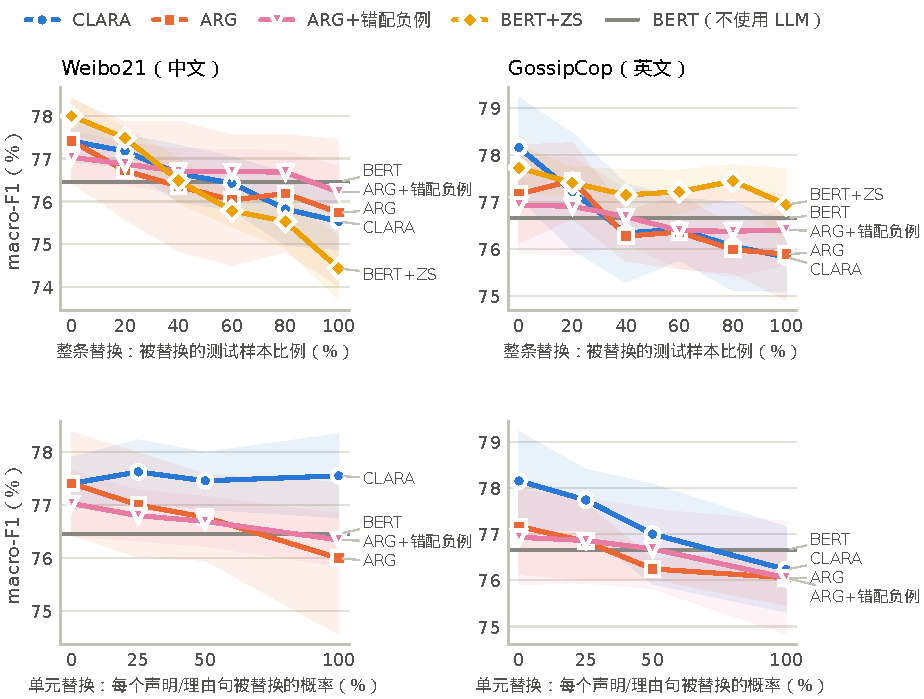
\includegraphics[width=\linewidth]{gen/figures/noise.pdf}
\caption{LLM 分析被替换时的 macro-F1}\label{fig:noise}
\note{上：整条替换；下：单元替换。阴影为种子间标准差，灰色横线为不使用 LLM 的 BERT。FactGuard 的下降幅度远大于其余方法，为保持纵轴的分辨率未画出；全部数值见表~\ref{tab:noise}。}
\end{figure}

\subsubsection{相关性门控能识别不属于该新闻的分析}
表~\ref{tab:gate} 显示，相关性门控 $r$ 几乎完美地区分了属于本新闻的分析单元与被替换进来的单元：整条替换时 AUC 为 \fthree{CN/gate/relevance/item/auc_r}（Weibo21）与 \fthree{EN/gate/relevance/item/auc_r}（GossipCop），单元替换时为 \fthree{CN/gate/relevance/unit/auc_r} 与 \fthree{EN/gate/relevance/unit/auc_r}。属于本新闻的单元平均 $r$ 在 0.93 以上，被替换的单元在 0.2 以下。判定门控 $g$ 则完全不具备这一能力（AUC 约 0.5）。

\begin{table}[htbp]
\centering\small
\caption{相关性门控对“分析单元是否属于该新闻”的区分能力}\label{tab:gate}
\fittable{gen/tables/gate.tex}
\note{测试集，多种子均值。}
\end{table}

\subsubsection{去掉相关性门控后模型在替换下崩溃}
消融实验（表~\ref{tab:ablation}）中“去掉相关性门控与错配负例”的变体，在全部分析被整条替换时，macro-F1 只有 \ptwo{CN/ablation/no_relevance/noise100/mean}（Weibo21）与 \ptwo{EN/ablation/no_relevance/noise100/mean}（GossipCop），远低于不使用 LLM 的 BERT。带相关性门控的完整模型在同样条件下为 \ptwo{CN/noise/clara/item/100/mean} 与 \ptwo{EN/noise/clara/item/100/mean}，比 BERT 低 \ptwo{CN/derived/clara_item100_gap} 与 \ptwo{EN/derived/clara_item100_gap} 个点。

\subsubsection{声明被逐条替换时，\method{} 可以丢弃声明而保留整体判断}
当分析中的声明被逐条替换时，\method{} 逐条关闭被替换声明的相关性门控，其余部分照常使用。在 Weibo21 上，即使全部声明都被替换，\method{} 的 macro-F1 仍为 \ptwo{CN/noise/clara/unit/100/mean}，与未替换时（\ptwo{CN/noise/clara/unit/0/mean}）持平。这一结果需要谨慎解读，因为两类方法在该条件下保留的信息不同：\method{} 的整体判断与零样本评分不由声明构成，因而没有被替换；ARG 的理由是一段自由文本，全部句子被替换后不再含有任何属于该新闻的 LLM 信息，这一条件对它几乎等同于整条替换（\ptwo{CN/noise/arg/unit/100/mean} 对 \ptwo{CN/noise/arg/item/100/mean}）。因此，此时 \method{} 比 ARG 高出的 \ptwo{CN/noise_sig/unit100/arg/diff_mean} 个点（$p_{\text{样本}}\peq{CN/noise_sig/unit100/arg/bootstrap/p}$，$p_{\text{种子}}\peq{CN/noise_sig/unit100/arg/welch_p}$；全精度复核中为 \ptwo{CN/fp32/clara_vs/arg_unit100/diff_mean} 个点，两种检验都成立，见附录~\ref{app:live}）说明的是结构上的一个性质：声明受到污染时，\method{} 可以只丢弃声明、继续使用整体判断；它并不说明在保留同等信息的条件下 \method{} 更稳健。当每个单元以一半的概率被替换时，两者相差 \ptwo{CN/noise_sig/unit50/arg/diff_mean} 个点，不显著。在 GossipCop 上，\method{} 从 \ptwo{EN/noise/clara/unit/0/mean} 降到 \ptwo{EN/noise/clara/unit/100/mean}，与 ARG（\ptwo{EN/noise/arg/unit/100/mean}）相当：如 \ref{sec:exp-gate} 节所示，该数据集上 \method{} 的判定更多依赖声明实例，丢弃声明的代价更大（\ref{sec:exp-ablation} 节的消融进一步显示，此时它低于从未使用声明的变体）。

\subsubsection{需要如实说明的两点}
第一，ARG 本身对替换就相当稳健：整条替换全部理由后，它在两个数据集上只下降 \ptwo{CN/derived/arg_item100_drop} 与 \ptwo{EN/derived/arg_item100_drop} 个点。它的融合权重并不能识别被替换的理由（被替换与未被替换样本上的平均权重几乎相同，区分两者的 AUC 为 \fthree{CN/gate/weights_under_noise/arg/auc} 与 \fthree{EN/gate/weights_under_noise/arg/auc}），稳健性来自新闻文本在其表示中占主导。给 ARG 加上同样的错配负例训练后，它在全部分析被整条替换时比 \method{} 高 \ptwo{CN/derived/argswap_minus_clara_item100}（Weibo21）与 \ptwo{EN/derived/argswap_minus_clara_item100}（GossipCop）个点，差异不显著。因此，“在分析不可用时保持稳健”并不是 \method{} 独有的性质：在两类方法都失去全部 LLM 信息的整条替换下，\method{} 与 ARG 没有差别。第二，FactGuard 对两种替换都非常敏感（整条替换全部分析后降到 \ptwo{CN/noise/factguard/item/100/mean} 与 \ptwo{EN/noise/factguard/item/100/mean}），因为它用 LLM 抽取的 topic-content 代替新闻原文参与交叉注意力。

\subsubsection{相关性门控识别的是话题层面的不匹配}
被替换进来的分析来自另一条新闻，与原文在话题上就不一致。为了检验相关性门控能否识别更细微的不匹配，我们把单句事实篡改集（\ref{sec:robust-sets} 节）中篡改后的文本与其\emph{原文}的 LLM 分析配对：此时分析与文本话题相同，只有对应被改句子的那条声明与文本在一处事实上不符。表~\ref{tab:cross} 显示相关性门控对此没有反应：对应被改句子的声明与其余声明的平均 $r$ 相同，用 $r$ 区分两者的 AUC 为 \fthree{CN/cross/cross/auc_r_unfaithful} 与 \fthree{EN/cross/cross/auc_r_unfaithful}。相关性门控能挡住的是“分析说的不是这条新闻”，挡不住“分析在某个事实上与这条新闻不符”。后者正是 LLM 幻觉更常见的形态，因此不能把相关性门控理解为对幻觉的一般性防护。

\begin{table}[htbp]
\centering\small
\caption{篡改后的文本搭配不同分析时的平均相关性门控 $r$}\label{tab:cross}
\fittable{gen/tables/cross.tex}
\note{分别搭配它自己的分析与原文的分析，按实例类别统计；3 个种子。}
\end{table}

\subsection{判定门控学到了什么}\label{sec:exp-gate}

判定门控 $g$ 的设计意图是估计“LLM 在该实例上是否站对了边”。表~\ref{tab:gate-cells} 按 LLM 的整体判断与新闻标签把测试样本分为四组，给出各组的平均 $g_0$。

\begin{table}[htbp]
\centering\small
\caption{判定门控在整体实例上的取值}\label{tab:gate-cells}
\fittable{gen/tables/gate_cells.tex}
\note{测试集，多种子均值。若门控跟随“LLM 是否正确”，则第一、四行应高，第二、三行应低。}
\end{table}

\subsubsection{判定门控跟随的是新闻标签，而不是 LLM 的正误}
在 Weibo21 上，$g_0$ 在两组假新闻上都高（约 0.81），在两组真新闻上都低（约 0.63--0.66），与 LLM 判断的方向无关：它预测“LLM 是否正确”的 AUC 为 \fthree{CN/gate/clara/overall/auc_gate/mean}，预测“新闻是否为假”的 AUC 却有 \fthree{CN/gate/clara/overall/auc_gate_for_label/mean}。在 GossipCop 上情形相反，$g_0$ 在真新闻上更高，对“LLM 是否正确”的 AUC 为 \fthree{EN/gate/clara/overall/auc_gate/mean}，但这同样可以由标签解释：该数据集上 LLM 多数时候判真，“LLM 正确”与“新闻为真”高度重合。也就是说，一个能看到新闻文本的门控学到的是“这条新闻像不像假新闻”，并据此调节 LLM 证据的权重。它起到的是让 LLM 证据的权重随文本先验变化的作用，而不是可靠性估计。

\subsubsection{这一现象并非 \method{} 独有}
ARG 的理由可用性预测器对“该理由对应的 LLM 判断是否正确”的 AUC 看起来不低（表~\ref{tab:useful}），但决定融合权重的打分模块对同一目标的 AUC 只有 0.50--0.55（加入错配负例训练后为 0.45--0.67）。可用性预测器同时读取新闻与理由：新闻文本提示标签，理由文本提示 LLM 的判断，两者一比较即可得到监督目标。表中“自身预测”一列用 ARG 最终的预测概率与 LLM 判断是否一致来预测同一目标，不需要任何专门的模块，得到的 AUC 与可用性预测器相当或更高。可见可用性预测器并没有提供分类器自身判断之外的信息。

\begin{table}[htbp]
\centering\small
\caption{对“该理由对应的 LLM 判断是否正确”的 AUC}\label{tab:useful}
\fittable{gen/tables/useful.tex}
\note{测试集，多种子均值。三列分别为 ARG 的可用性预测器、融合权重，以及“ARG 自身的最终预测与 LLM 判断是否一致”。}
\end{table}

\subsubsection{LLM 自身的置信度也不提供这一信息}
LLM 评分偏离 0.5 的程度对其判断是否正确的 AUC 只有 \fthree{CN/gate/clara/overall/auc_llm_conf/mean} 与 \fthree{EN/gate/clara/overall/auc_llm_conf/mean}。真正有信息量的是“文本分支是否同意 LLM”（AUC \fthree{CN/gate/clara/overall/auc_text_agreement/mean} 与 \fthree{EN/gate/clara/overall/auc_text_agreement/mean}），而这一信息在加性融合中已经被隐式使用。综合来看，在闭卷条件下我们没有找到能够估计“LLM 的判断是否可靠”且不退化为预测标签的信号；本文最初设想的“声明级可靠性门控”在这一含义上没有成立，成立的是相关性门控所回答的那个更窄的问题。

\subsubsection{实例概率的分布}
两个数据集上承担判定的实例不同。在 Weibo21 的假新闻中，至少有一条声明 $p_k>0.5$ 的占 \pone{CN/gate/clara/flag/fake_any_claim/mean}\%，只有整体实例 $p_0>0.5$ 的占 \pone{CN/gate/clara/flag/fake_overall_only/mean}\%，可见这里新闻级的判定主要由整体实例承担。在 GossipCop 的假新闻中，至少有一条声明 $p_k>0.5$ 的占 \pone{EN/gate/clara/flag/fake_any_claim/mean}\%，而只由整体实例触发的不到 1\%：该数据集上 LLM 的整体判断区分度很低（零样本判断的 AUC 仅 \pone{EN/style_llm/zero-shot P(fake)/auc_orig}\%），裁决器转而依靠声明实例。

\subsection{风格改写}\label{sec:exp-style}

\begin{table}[htbp]
\centering\small
\caption{风格改写前后的 macro-F1（\%）}\label{tab:style}
\fittable{gen/tables/style.tex}
\note{只统计成功改写的样本，“原文”为同一批样本改写前的结果。分隔线以下两行是只读取 LLM 输出文本、不读新闻原文的 BERT。}
\end{table}

\subsubsection{所有闭卷检测器都主要依赖文风}
把假新闻改写为通稿文风、真新闻改写为营销号文风后，Weibo21 上所有 SLM 类方法的 macro-F1 从 76--78 降到 50--53，接近随机；GossipCop 上从 77--78 降到 65--69（表~\ref{tab:style}）。读取 LLM 理由并不能使检测器摆脱对文风的依赖。在 Weibo21 上，改写后各 SLM 类方法与 BERT 的差异都不显著。在 GossipCop 上，FactGuard 与 \method{} 改写后分别比 BERT 高 \ptwo{EN/style/_vs_bert/factguard/diff_mean} 与 \ptwo{EN/style/_vs_bert/clara/diff_mean} 个点，差异显著；这两种方法都使用了 LLM 对新闻内容的重新表述（topic-content 或声明），其文风与原文不同，ARG 则没有这一差别（\ptwo{EN/style/_vs_bert/arg/diff_mean} 个点）。直接微调的 LoRA-LLM 下降最少（Weibo21 上 \ptwo{CN/derived/lora_style_drop} 个点，GossipCop 上 \ptwo{EN/derived/lora_style_drop} 个点），改写后在两个数据集上都显著高于 BERT，但在 Weibo21 上也只剩 \ptwo{CN/style/lora/style/mean}。

\subsubsection{只读 LLM 复述的分类器：更稳健，但暴露了分布内精度的来源}
表~\ref{tab:style} 分隔线以下的两行是不读新闻原文、只读 LLM 输出的 BERT：一行读 FactGuard 式的 topic-content 摘要，一行读 \method{} 抽取的声明。在 GossipCop 上，只读摘要的 BERT 在原始测试集上为 \ptwo{EN/main/bert_tc/macf1}，不低于读原文的 BERT（\ptwo{EN/main/bert/macf1}），风格改写后仍有 \ptwo{EN/style/bert_tc/style/mean}，比读原文的 BERT 高 \ptwo{EN/style/_vs_bert/bert_tc/diff_mean} 个点；只读声明的 BERT 改写后为 \ptwo{EN/style/bert_claims/style/mean}。在 Weibo21 上，只读摘要的 BERT 改写后为 \ptwo{CN/style/bert_tc/style/mean}，同样显著高于读原文的 BERT（\ptwo{CN/style/bert/style/mean}），但它在原始测试集上只有 \ptwo{CN/main/bert_tc/macf1}，比读原文低 \ptwo{CN/derived/bert_minus_bert_tc} 个点。这两个数值与 FactGuard 论文中“仅用 topic-content”的消融结果（69.0 与 76.9）\citep{he2026factguard}一致。它们说明两点：第一，让 LLM 先用中性的措辞复述新闻，确实能削弱检测器对文风的依赖；第二，在 Weibo21 上，去掉文风的代价约为 6 个点，分布内精度中有相当一部分来自文风。声明并不总是风格中性的：在以短帖为主的 Weibo21 上，LLM 抽取的声明基本沿用原文措辞，只读声明的 BERT 改写后只有 \ptwo{CN/style/bert_claims/style/mean}，低于随机。

\subsubsection{LLM 自身的判断同样依赖文风}
表~\ref{tab:style-llm} 不涉及任何训练，只比较 Qwen2.5-7B 对同一批样本改写前后的评分。零样本判断的 AUC 在 Weibo21 上从 \pone{CN/style_llm/zero-shot P(fake)/auc_orig} 降到 \pone{CN/style_llm/zero-shot P(fake)/auc_style}，在 GossipCop 上从 \pone{EN/style_llm/zero-shot P(fake)/auc_orig} 降到 \pone{EN/style_llm/zero-shot P(fake)/auc_style}。声明级怀疑度在改写后对真假新闻几乎没有区分度。这说明 LLM 在闭卷条件下给出的“常识分析”“声明核查”，其判别力主要来自文本的表面特征，而不是对事实的掌握。把 LLM 的分析拆得更细并不能改变这一点：声明是从改写后的文本中抽取的，其措辞与评分仍然随文风变化。

\begin{table}[htbp]
\centering\small
\caption{Qwen2.5-7B 的评分在风格改写前后对真假新闻的区分能力}\label{tab:style-llm}
\fittable{gen/tables/style_llm.tex}
\note{不涉及训练。均值差为假新闻与真新闻平均评分之差。}
\end{table}

\subsection{单句事实篡改：敏感性与定位}\label{sec:exp-loc}

\begin{table}[htbp]
\centering\small
\caption{各方法对单句事实篡改的敏感性（\%）}\label{tab:tamper}
\fittable{gen/tables/tamper.tex}
\note{“判假”为被判为假的比例；成对正确率为篡改后样本的预测概率高于其原文的比例，50\% 相当于随机。}
\end{table}

\subsubsection{SLM 类方法对局部事实改动几乎没有反应}
表~\ref{tab:tamper} 显示，把真新闻中的一句话改成与原文事实不符的陈述后，各 SLM 类方法判其为假的比例几乎不变（例如 \method{} 在 Weibo21 上从 \pone{CN/localisation/_sensitivity/clara/flag_rate_original}\% 变为 \pone{CN/localisation/_sensitivity/clara/flag_rate_tampered}\%）；篡改后的预测概率高于原文的比例只有 53\%--55\%，略高于随机。BERT+ZS 稍高（\pone{CN/localisation/_sensitivity/bert_zs/pairwise_acc}\% 与 \pone{EN/localisation/_sensitivity/bert_zs/pairwise_acc}\%），因为 LLM 的零样本评分对部分改动有反应。直接微调的 LoRA-LLM 最敏感，成对正确率为 \pone{CN/localisation/_sensitivity/lora/pairwise_acc}\% 与 \pone{EN/localisation/_sensitivity/lora/pairwise_acc}\%，但它判假的比例同样变化很小（Weibo21 上从 \pone{CN/localisation/_sensitivity/lora/flag_rate_original}\% 到 \pone{CN/localisation/_sensitivity/lora/flag_rate_tampered}\%）：预测概率朝正确的方向移动了，幅度却远不足以改变判定。这与风格改写的结果一致：这些检测器学到的主要不是“内容是否属实”。需要强调，篡改后的句子只是与原文不符，未必在现实中为假，这项测试衡量的是模型对事实内容变化的敏感程度。

\begin{table}[htbp]
\centering\small
\caption{被篡改句子的定位结果（\%）}\label{tab:loc}
\fittable{gen/tables/loc.tex}
\note{“单位”为方法给出分数的粒度；声明级分数通过声明所在的句子编号映射到句子。分隔线以下为 \method{} 与 \student{} 的消融变体。}
\end{table}

\subsubsection{定位结果只略高于随机}
在定位任务上（表~\ref{tab:loc}），\method{} 的 Hit@1 在 Weibo21 上为 \pone{CN/localisation/CLARA/hit@1}\%，随机猜测为 \pone{CN/localisation/CLARA/chance}\%；在 GossipCop 上为 \pone{EN/localisation/CLARA/hit@1}\%，随机为 \pone{EN/localisation/CLARA/chance}\%。训练后的裁决器并没有比直接使用 LLM 的怀疑度评分更好（\pone{CN/localisation/LLM suspicion scores/hit@1}\% 与 \pone{EN/localisation/LLM suspicion scores/hit@1}\%），各消融变体也都在同一水平。表中最好的是对 LoRA-LLM 做遮挡归因（Weibo21 上 \pone{CN/localisation/LoRA-LLM + occlusion/hit@1}\%），它不需要任何声明级结构。\method{} 的定位受两方面限制：LLM 抽取的声明只覆盖了 \pone{CN/localisation/_claim_coverage}\%（Weibo21）与 \pone{EN/localisation/_claim_coverage}\%（GossipCop）的被篡改句子；即使覆盖到，LLM 对这条声明的怀疑度也往往不比其他声明高。“只用新闻级标签即可获得声明级定位”这一预期在闭卷条件下没有实现。

\subsection{消融实验}\label{sec:exp-ablation}

\begin{table}[htbp]
\centering\footnotesize
\setlength{\tabcolsep}{3.4pt}
\caption{\method{} 的消融实验（macro-F1，\%）}\label{tab:ablation}
\fittable{gen/tables/ablation.tex}
\note{“整条替换”与“单元替换”分别为全部测试样本的分析被整条替换、全部声明被逐条替换时的结果。Weibo21 为 5 个种子，GossipCop 为 3 个种子。$^{*}$ 表示在同一评测条件下与完整模型的差异显著（两种检验均 $p<0.05$，未做多重比较校正）。}
\end{table}

表~\ref{tab:ablation} 逐一去掉或替换 \method{} 的组件。Weibo21 为 5 个种子；GossipCop 为 \cnt{EN/ablation/_seeds_count} 个种子，表中“完整”一行取同样的种子（\ptwo{EN/ablation/full/test/mean}），因此与表~\ref{tab:main} 中 5 个种子的数值不同。

\subsubsection{两个数据集上一致的结论：论证文本、声明分解与判定门控对精度没有可测的贡献}
去掉全部论证文本、只保留评分，macro-F1 在 Weibo21 上为 \ptwo{CN/ablation/no_args/test/mean}（完整模型 \ptwo{CN/ablation/full/test/mean}），在 GossipCop 上为 \ptwo{EN/ablation/no_args/test/mean}（完整模型 \ptwo{EN/ablation/full/test/mean}），差异都不显著。只保留整体实例而去掉全部声明（\ptwo{CN/ablation/no_claims/test/mean} 与 \ptwo{EN/ablation/no_claims/test/mean}）、去掉判定门控（\ptwo{CN/ablation/no_gate/test/mean} 与 \ptwo{EN/ablation/no_gate/test/mean}）、整条新闻共用一个判定门控、把 noisy-OR 换成注意力聚合、允许实例证据读取整条新闻，在原始测试集上与完整模型的差异同样都不显著。本文方法的核心设想是让小模型阅读并裁决声明级的正反论证；就分布内精度而言，这一设想中的每个部件都可以去掉而不产生可测的损失。

\subsubsection{LLM 评分的作用因数据集而异}
在 Weibo21 上，去掉评分、只保留论证文本，macro-F1 降到 \ptwo{CN/ablation/no_v/test/mean}，显著低于完整模型，也低于不使用 LLM 的 BERT（\ptwo{CN/main/bert/macf1}）；把论证前的整体评分从零样本判断换成提示内的第一印象（即严格的单次调用），降到 \ptwo{CN/ablation/fi_score/test/mean}，同样显著。也就是说，在这个数据集上 \method{} 相对 BERT 的提升几乎全部来自 LLM 的数值评分，尤其是单独一次调用得到的零样本评分，这与 BERT+ZS 的结果（\ref{sec:main-results} 节）相互印证。在 GossipCop 上情形不同：去掉评分后为 \ptwo{EN/ablation/no_v/test/mean}，换成第一印象后为 \ptwo{EN/ablation/fi_score/test/mean}，都不显著。该数据集上 LLM 评分的区分度本来就低（零样本判断的 AUC 为 \pone{EN/style_llm/zero-shot P(fake)/auc_orig}\%）。除整体文本分支外，GossipCop 上没有任何单个组件的去除造成显著下降，\method{} 相对 BERT 的差距（本身不显著）无法归因到某个具体组件。

\subsubsection{相关性门控与整体文本分支决定了稳健性}
去掉相关性门控与错配负例不显著影响原始测试集上的精度（\ptwo{CN/ablation/no_relevance/test/mean} 与 \ptwo{EN/ablation/no_relevance/test/mean}），但全部分析被整条替换时，macro-F1 降到 \ptwo{CN/ablation/no_relevance/noise100/mean} 与 \ptwo{EN/ablation/no_relevance/noise100/mean}，比完整模型低 \ptwo{CN/ablation/no_relevance/vs_full_noise100/diff_mean} 与 \ptwo{EN/ablation/no_relevance/vs_full_noise100/diff_mean} 个点，比 BERT 低 \ptwo{CN/derived/no_relevance_gap} 与 \ptwo{EN/derived/no_relevance_gap} 个点。整体文本分支是唯一在两个数据集的原始测试集上都显著的组件（去掉后下降 \ptwo{CN/ablation/no_global/vs_full/diff_mean} 与 \ptwo{EN/ablation/no_global/vs_full/diff_mean} 个点）；没有它，分析被整条替换时模型在 GossipCop 上降到 \ptwo{EN/ablation/no_global/noise100/mean}，相当于恒定预测。

\subsubsection{丢弃被替换的声明并不总是没有代价}
\ref{sec:exp-noise} 节指出，声明被逐条替换时 \method{} 可以丢弃声明、依靠整体实例。Weibo21 上的消融印证了这一机制：去掉整体实例的变体在全部声明被替换时降到 \ptwo{CN/ablation/no_overall/unit100/mean}，显著低于完整模型（\ptwo{CN/ablation/full/unit100/mean}）。但在 GossipCop 上，完整模型在同一条件下为 \ptwo{EN/ablation/full/unit100/mean}，显著低于从一开始就不使用声明的变体（\ptwo{EN/ablation/no_claims/unit100/mean}，该变体不受声明替换影响）。相关性门控识别出了被替换的声明，但裁决器在该数据集上平时依赖声明实例（\ref{sec:exp-gate} 节），退回之后的表现不如从未使用声明的模型。

\subsection{学生模型}\label{sec:exp-distill}

\begin{table}[htbp]
\centering\small
\caption{推理时不调用 LLM 的学生模型（macro-F1，\%）}\label{tab:distill}
\fittable{gen/tables/distill.tex}
\note{3 个种子。“其教师”为同一次运行中训练的教师模型的结果；$^{*}$ 表示与同样种子的 BERT 相比差异显著。}
\end{table}

\subsubsection{蒸馏得到的学生都没有显著超过 BERT}
表~\ref{tab:distill} 给出三种方法的学生模型。在 Weibo21 上，ARG-D（\ptwo{CN/distill/arg_d/test/mean}）与同样种子的 BERT（\ptwo{CN/distill/bert/test/mean}）持平，FactGuard-D（\ptwo{CN/distill/factguard_d/test/mean}）与 \student{}（\ptwo{CN/distill/clara_d/test/mean}）略低，差异都不显著。在 GossipCop 上 \student{} 为 \ptwo{EN/distill/clara_d/test/mean}，比 BERT 高 \ptwo{EN/distill/clara_d/vs_bert/diff_mean} 个点，但差异不显著（$p_{\text{样本}}\peq{EN/distill/clara_d/vs_bert/bootstrap/p}$，$p_{\text{种子}}\peq{EN/distill/clara_d/vs_bert/welch_p}$）；ARG-D 与 BERT 持平，FactGuard-D 更低。各教师模型本身相对同种子 BERT 的优势只有 0.3--1.6 个点且大多不显著，学生再损失一部分之后，“把 LLM 的知识蒸馏进小模型”在本文的设置下没有留下可测的收益。原论文报告 ARG-D 比 BERT 高约 1.3--1.8 个点\citep{hu2024bad}，在本文的多种子复现中没有重现。

\subsubsection{声明到句子的对齐蒸馏没有带来定位能力}
\student{} 的设计目标之一是保留句级定位。表~\ref{tab:loc} 显示这一目标没有实现：它在 Weibo21 上的 Hit@1 为 \pone{CN/localisation/CLARA-D/hit@1}\%，与随机猜测（\pone{CN/localisation/CLARA-D/chance}\%）相同；在 GossipCop 上为 \pone{EN/localisation/CLARA-D/hit@1}\%（随机 \pone{EN/localisation/CLARA-D/chance}\%）。去掉实例级蒸馏、甚至完全不用教师的句子级 MIL 变体，定位结果都在同一水平。教师的声明级概率本身几乎不含位置信息（\ref{sec:exp-loc} 节），对齐到句子之后自然无从蒸馏。

\subsection{未见领域}\label{sec:exp-lodo}

\begin{table}[htbp]
\centering\small
\caption{Weibo21 留一领域实验的 macro-F1（\%）}\label{tab:lodo}
\fittable{gen/tables/lodo.tex}
\note{3 个种子；训练与验证数据不含被留出的领域。每行最优者加粗，$^{*}$ 表示各领域平均值显著高于 BERT。}
\end{table}

表~\ref{tab:lodo} 给出六个领域的留一领域结果。各领域的测试集只有一百到四百条，单个领域上的数值波动很大，下面只讨论各领域的平均值；它的检验采用按领域分层的 bootstrap 与对种子的 Welch 检验。

\subsubsection{在未见领域上有帮助的仍然是 LLM 的零样本评分}
BERT+ZS 的平均 macro-F1 为 \ptwo{CN/lodo/_macro_avg/bert_zs}，比 BERT 高 \ptwo{CN/derived/lodo_bert_zs_minus_bert} 个点，差异显著（$p_{\text{样本}}\peq{CN/lodo/_vs_bert/bert_zs/bootstrap/p}$，$p_{\text{种子}}\peq{CN/lodo/_vs_bert/bert_zs/welch_p}$），在六个领域中的四个上最高。LLM 的判断不依赖训练数据的领域分布，把它作为一个加性的先验，领域变化时仍然有效。

\subsubsection{\method{} 与 ARG 在未见领域上没有超过 BERT}
ARG 与 \method{} 的平均值为 \ptwo{CN/lodo/_macro_avg/arg} 与 \ptwo{CN/lodo/_macro_avg/clara}，与 BERT（\ptwo{CN/lodo/_macro_avg/bert}）没有差别。\method{} 显著低于 BERT+ZS（相差 \ptwo{CN/derived/lodo_clara_minus_bert_zs} 个点，$p_{\text{样本}}\peq{CN/lodo/_vs_bert_zs/clara/bootstrap/p}$，$p_{\text{种子}}\peq{CN/lodo/_vs_bert_zs/clara/welch_p}$），尽管它同样读入了零样本评分。一个可能的原因是，\method{} 对该评分的使用要经过在训练领域上拟合的门控与证据模块（\ref{sec:exp-gate} 节显示判定门控跟随的是文本的标签倾向），这些模块本身带有领域依赖；而 BERT+ZS 只用一个标量权重。这是更复杂的协同结构相对简单融合的一个明确的劣势。

\subsection{拒答}\label{sec:exp-selective}

\begin{table}[htbp]
\centering\small
\caption{选择性预测的结果}\label{tab:selective}
\fittable{gen/tables/selective.tex}
\note{多种子均值。AURC 越低越好；其余各列为只保留置信度最高的一部分样本时的准确率（\%），覆盖率 100\% 即不拒答。“选择器”为在验证集上拟合的逻辑回归。}
\end{table}

\begin{figure}[htbp]
\centering
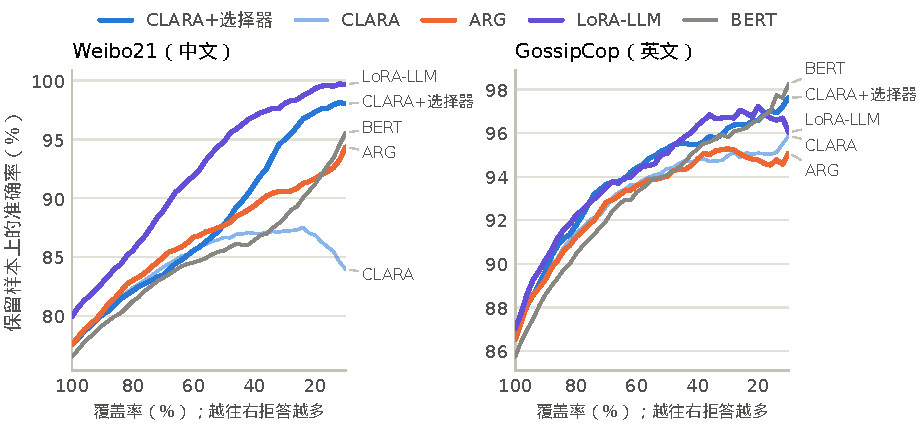
\includegraphics[width=\linewidth]{gen/figures/selective.pdf}
\caption{保留样本上的准确率随覆盖率的变化}\label{fig:selective}
\note{多种子均值。浅色线为 \method{} 直接用 $|\hat y-0.5|$ 作为置信度的结果；数值见表~\ref{tab:selective}。}
\end{figure}

\subsubsection{直接使用 LLM 评分会损害置信度排序}
表~\ref{tab:selective} 中，以 $|\hat y-0.5|$ 为置信度时，Weibo21 上 \method{} 的 AURC（\ptwo{CN/selective/clara/maxprob/aurc}）比 BERT（\ptwo{CN/selective/bert/maxprob/aurc}）更差，BERT+ZS 与 FactGuard 也是如此。问题出在最有把握的那部分预测：只保留置信度最高的 10\% 样本时，BERT 的准确率为 \pone{CN/selective/bert/maxprob/acc@10}\%，\method{} 只有 \pone{CN/selective/clara/maxprob/acc@10}\%，BERT+ZS 为 \pone{CN/selective/bert_zs/maxprob/acc@10}\%。原因在于 LLM 的零样本评分高度两极化而且过于自信：Weibo21 测试集中有 \pone{CN/zs_calibration/hi_share}\% 的样本 $p_{\mathrm{zs}}>0.95$，其中实际为假的只有 \pone{CN/zs_calibration/hi_fake_rate}\%。把它的 logit 加到输出上，这批样本就被整体推到置信度的最高端：\method{} 置信度最高的 10\% 预测中有 \pone{CN/selective/clara/maxprob/top10_fake_share}\% 判假（BERT 为 \pone{CN/selective/bert/maxprob/top10_fake_share}\%），这一侧的准确率只有 \pone{CN/selective/clara/maxprob/top10_acc_fake_side}\%，判真的一侧则为 \pone{CN/selective/clara/maxprob/top10_acc_real_side}\%。\method{} 与 BERT+ZS 都没有对 LLM 的评分做校准，这是两者共同的缺陷。GossipCop 上 LLM 很少给出接近 1 的评分（$p_{\mathrm{zs}}>0.95$ 的样本占 \pone{EN/zs_calibration/hi_share}\%），这一现象不明显。

\subsubsection{选择器可以修复这一问题，但不构成优势}
用裁决器的内部信号在验证集上拟合选择器后，\method{} 在 Weibo21 上的 AURC 降到 \ptwo{CN/selective/clara/selector/aurc}，置信度最高的 10\% 样本准确率回到 \pone{CN/selective/clara/selector/acc@10}\%。这一 AURC 在 SLM 类方法中数值最低：对随机种子的 Welch 检验显示它低于 BERT 与 BERT+ZS（$p\peq{CN/selective/_selector_vs/bert/maxprob/welch_p}$ 与 $\fthree{CN/selective/_selector_vs/bert_zs/maxprob/welch_p}$），但与同样拟合了选择器的 ARG（\ptwo{CN/selective/arg/selector/aurc}）没有可分辨的差别（$p\peq{CN/selective/_selector_vs/arg/selector/welch_p}$），并且远不及 LoRA-LLM（\ptwo{CN/selective/lora/maxprob/aurc}）。AURC 没有做对测试样本的 bootstrap，这些 $p$ 值只供参考。覆盖率为 50\% 时，\method{} 加选择器的准确率为 \pone{CN/selective/clara/selector/acc@50}\%，ARG 加选择器为 \pone{CN/selective/arg/selector/acc@50}\%。GossipCop 上各方法的 AURC 都在 5--7 之间，BERT+ZS 最低（\ptwo{EN/selective/bert_zs/maxprob/aurc}），\method{} 加选择器为 \ptwo{EN/selective/clara/selector/aurc}。总体上，\method{} 的内部信号可以用来纠正它自身的置信度排序，但没有带来超出其他方法的拒答能力；原设想中“两分支分歧与门控提供不可判信号”没有得到支持。

\subsection{更换分析用的 LLM}\label{sec:exp-llm2}

\begin{table}[htbp]
\centering\footnotesize
\setlength{\tabcolsep}{3.6pt}
\caption{更换分析用 LLM 后的 macro-F1（\%）}\label{tab:llm2}
\fittable{gen/tables/llm2.tex}
\note{把 Qwen2.5-7B 换成 Qwen3-8B，3 个种子（Qwen2.5 一列取相同的种子）；各方法沿用在 Qwen2.5 上选出的学习率。“整条替换”为全部测试样本的 LLM 输出被替换。}
\end{table}

为了检验结论是否依赖于某一个 LLM，我们用 Qwen3-8B（关闭思考模式）重新生成全部 LLM 输出，并重新训练依赖 LLM 输出的四种方法（表~\ref{tab:llm2}）。

\subsubsection{分布内的结论不变}
换用 Qwen3-8B 后，四种方法在两个数据集上的变化都在 1.5 个点以内，彼此之间仍然相差不到 2 个点。在两个 LLM 与两个数据集构成的四种组合中，\method{} 在三种上数值最高（Weibo21 上使用 Qwen2.5 时 BERT+ZS 最高），但对第二名的领先都不到 1 个点，在 3 个种子下不足以说明问题。

\subsubsection{相关性门控是软门控，残余的泄漏随运行而变}
换用 Qwen3-8B 后，相关性门控区分两类分析单元的 AUC 仍在 0.99 左右，但被替换单元上的平均 $r$ 在 Weibo21 上从 \ftwo{CN/llm2/relevance_first/item/r_foreign} 升到 \ftwo{CN/llm2/relevance_second/item/r_foreign}：门控把它们排在了后面，却没有把它们压到接近 0。由于 $r$ 是连续的乘性系数，这些单元的证据仍有一部分进入判定，\method{} 在全部分析被整条替换时降到 \ptwo{CN/llm2/clara/second_noise100/mean}，低于同条件下的 ARG（\ptwo{CN/llm2/arg/second_noise100/mean}）与不使用 LLM 的 BERT。在 GossipCop 上情形相反，\method{} 为 \ptwo{EN/llm2/clara/second_noise100/mean}，ARG 降到 \ptwo{EN/llm2/arg/second_noise100/mean}。因此，\ref{sec:exp-noise} 节中“整条替换下 \method{} 与 ARG 相当”的结论，更准确的表述是两者互有高低、没有系统性的差别；\method{} 的退回并不精确，其程度取决于门控被压低的幅度。推理时对 $r$ 取硬阈值可能缓解这一问题，本文没有验证。

\subsection{开销}\label{sec:exp-cost}

\begin{table}[htbp]
\centering\small
\caption{每条新闻的 LLM 开销}\label{tab:cost}
\fittable{gen/tables/cost.tex}
\note{平均输入与输出 token 数，以及单张 RTX 3090 上用 vLLM 批量生成时每千条新闻的耗时（秒）。$^\ddagger$ LoRA-LLM 的耗时用 Transformers 逐批前向测得，与 vLLM 不是同一推理实现，仅供量级参考。}
\end{table}

\begin{table}[htbp]
\centering\small
\caption{可训练参数量与单次训练耗时}\label{tab:train-cost}
\fittable{gen/tables/train_cost.tex}
\note{单张 RTX 3090；SLM 类方法使用冻结层缓存与混合精度，不含一次性的缓存构建。}
\end{table}

\subsubsection{\method{} 的 LLM 开销高于 ARG 与 FactGuard}
表~\ref{tab:cost} 显示，\method{} 的结构化调用要为每条声明输出两条论证，是各方法中最贵的：其输出 token 数在 Weibo21 上是 ARG 两条理由之和的 \ftwo{CN/cost/clara_over_arg/completion} 倍，在新闻更长、声明更多的 GossipCop 上是 \ftwo{EN/cost/clara_over_arg/completion} 倍；生成耗时分别是 \ftwo{CN/cost/clara_over_arg/seconds_per_1000} 倍与 \ftwo{EN/cost/clara_over_arg/seconds_per_1000} 倍。把辩论压缩到一次结构化调用，相对于每条新闻需要多次调用的辩论方法节省了调用次数，但相对于只需两段短理由的 ARG 与 FactGuard 并不便宜。BERT+ZS 只需要一次输出单个 token 的调用，是使用 LLM 的方法中最便宜的，而它的精度并不低（表~\ref{tab:main}）。

\subsubsection{训练与推理}
LoRA-LLM 推理时只做一次前向，开销与零样本判断同一量级，但需要对 7B 模型做一次约 \cnt{CN/lora_cost/train_seconds} 秒（Weibo21）的微调，并在部署时常驻一个 7B 模型。SLM 类方法在缓存冻结层之后单次训练不到 3 分钟（表~\ref{tab:train-cost}）；其中 ARG、FactGuard 与 \method{} 推理前都需要先完成表~\ref{tab:cost} 中的 LLM 生成。

\section{讨论}\label{sec:discussion}

\subsubsection{LLM 的理由文本为什么没有帮助}
消融实验中最直接的一条结果是：把 LLM 写的论证文本全部去掉、只留下它给出的评分，\method{} 在两个数据集上的精度都没有显著变化。BERT+ZS 与 ARG、FactGuard 的比较给出了同样的信息。一种解释是，在闭卷条件下 LLM 的分析文本本身不携带新闻原文之外的新信息：它是 LLM 对同一段文字的复述与评价，其中对判别有用的部分可以被压缩成一个倾向性分数，而小模型已经直接读到了新闻原文。分析文本只有在引入原文之外的内容（例如检索到的证据、LLM 确实掌握的背景事实）时才可能提供增量；\ref{sec:exp-style} 节的结果表明，至少对 7B 模型而言，后者很有限。

\subsubsection{为什么判定门控学不到“LLM 是否可靠”}
“LLM 在某个实例上是否站对了边”由两个量决定：LLM 表达的判断与该实例的真实状态。前者写在 LLM 的输出里，后者在闭卷条件下只能由新闻文本去推测。因此，一个读取新闻文本与 LLM 输出的门控，要预测这一目标，最直接的办法就是先从文本预测标签，再与 LLM 的判断比较。表~\ref{tab:gate-cells} 与表~\ref{tab:useful} 显示 \method{} 的判定门控与 ARG 的可用性预测器都落在这一解上。要得到不依赖标签预测的可靠性估计，需要第三个信息来源，例如外部证据，或 LLM 在同一问题上多次采样的一致性；后者是否有效留待后续工作检验。多示例学习的不对称性确实为真新闻中的声明提供了精确的监督，但这一监督同样可以由“这是一条真新闻”推出，并没有迫使模型去判断单条声明。

\subsubsection{多示例假设在多大程度上成立}
式~\eqref{eq:mil} 假设假新闻中存在可以单独指认的问题声明。\ref{sec:exp-gate} 节的统计显示，在 Weibo21 上多数假新闻是由整体实例而不是某条声明触发的。这与数据的性质有关：社交媒体上的不实消息常常整体是编造的，其中每条声明单独看都“像是可能发生的”，仅凭文本无法指出哪一条有问题。反过来，真新闻如实转述不实说法的情形会违反假设的另一半；我们在提示词中要求保留归属以减少这种情况，但没有通过人工标注去度量假设被违反的比例，这是本文的一个局限。

\subsubsection{关于任务本身}
风格改写与事实篡改两项测试指向同一个结论：在这两个常用数据集上，闭卷检测器学到的主要是真假新闻在写法上的差异。这与 Wu 等\citep{wu2024sheepdog}对 SLM 的观察一致，本文进一步表明它同样适用于 LLM 的闭卷判断，以及建立在这些判断之上的协同方法。把 LLM 的分析拆得更细、让它写出正反论证，改变的是分析的形式，而没有改变分析所依据的信息。对于“内容是否属实”这一问题，闭卷的 7B 模型既不掌握所需的事实，也没有表现出能从文本内部一致性中发现问题的能力。这提示：在不引入外部证据的前提下继续改进 LLM 与 SLM 的协同结构，在这类基准上能得到的主要是对文风线索更充分的利用；而声称具备“事实分析”能力的闭卷方法，应当接受风格受控的测试。

\subsubsection{对实践的建议}
如果目标只是分布内精度：在算力允许时直接微调 LLM；否则在 SLM 的输出上融合一个 LLM 零样本评分，成本最低且不逊于更复杂的结构。如果系统中确实要使用 LLM 生成的分析文本，本文的结果支持为它配一个相关性检查：它几乎不损失精度，却能避免在分析与新闻不符时性能大幅下降。无论采用哪种方案，方法间 1 个点以内的差异都需要多个随机种子与显著性检验才能判断。

\subsubsection{局限}
（1）分析用的 LLM 以 Qwen2.5-7B 为主，更强的模型可能掌握更多事实，结论未必外推到闭源大模型。（2）只使用了两个数据集，且都来自同一来源的时间划分。（3）风格改写与事实篡改由另一个 LLM 自动生成，事实是否保持只用数字串的保留比例做了粗略检查，没有人工核验；篡改后的句子与原文不符，但未必在现实中为假。生成这两个测试集的 Qwen3-8B 同时是 \ref{sec:exp-llm2} 节中的第二个分析模型，因此更换 LLM 的实验没有在这两个测试集上评测。（4）\method{} 的第一个版本曾在测试集上评估过一次，相关性门控是在看到那次结果后加入的（\ref{sec:protocol} 节）；虽然此后的选择只依据验证集，这仍然弱化了测试集的独立性。（5）主实验为节省算力使用了混合精度。全精度复核（附录~\ref{app:live}）没有改变定性结论，但显示 ARG 与 FactGuard 的数值对精度敏感，使用 GPT-3.5 理由的 ARG 在混合精度下比官方代码低 \ptwo{CN/official_arg/gap_cached} 个点；正文中 1 个点左右的差异不应被解读为方法之间的排序。（6）声明的质量、论证的质量以及定位结果都没有做人工评估。（7）\method{} 的超参数没有搜索，可能不是最优。

\section{本章小结}\label{sec:ch3-summary}

本章研究了闭卷条件下如何利用 LLM 的分析来检测虚假新闻，提出了声明级论证裁决方法 \method{}，并在统一 LLM、超参数搜索与随机种子的条件下，把它与 ARG、FactGuard、直接微调的 LLM 以及一个简单的评分融合基线做了比较。结论可以概括为三点。

第一，就方法而言，\method{} 在分布内与已有的协同方法持平，在未见领域上不如只融合一个 LLM 评分的简单基线；消融显示，论证文本、声明分解与判定门控对精度都没有可测的贡献。它的相关性门控是有效的，能可靠地识别与新闻对不上的分析单元，但回答的只是“分析是否属于这条新闻”，而不是“分析是否正确”。

第二，就这一类方法而言，我们没有找到能在闭卷条件下估计“LLM 的判断是否可靠”的信号：\method{} 的判定门控与 ARG 的可用性机制实际学到的都是对新闻标签的预测。

第三，就任务而言，风格改写与事实篡改两项测试表明，包括 LLM 自身判断在内的所有闭卷检测器主要依赖文风，对内容层面的事实改动几乎没有反应；把 LLM 的分析做得更细、更结构化，并不能改变它所依据的信息。

这些结果说明，要让检测器真正对“内容是否属实”作出反应，需要引入模型参数之外的信息。本章得到的三条经验将在下一章中直接使用：直接微调的 LLM 是比“冻结 LLM 加小模型”更强的骨干；用错配负例训练出的相关性判断是可靠的，可以从“分析是否属于这条新闻”迁移到“证据是否与这条声明有关”；任何声称利用了内容信息的方法，都应当与只看声明或只看文风的基线比较，并接受输入受控的测试。第~\ref{ch:openbook}~章据此转向带有外部证据的设定。

\chapter{证据驱动的声明验证方法}\label{ch:openbook}

第~\ref{ch:clara}~章表明，在不引入外部信息的条件下，把 LLM 的分析做得更细并不能改变检测器主要依赖文风这一事实。本章转向\emph{开卷}设定：每条待核查的声明附带一组从网络检索到的原始报道，模型需要从中找出证据并据此判断声明的真实性等级。本章要回答三个问题：证据究竟能带来多大的提升；现有数据集中的“证据”是否泄漏了结论；一个可在单张显卡上训练的 LLM 验证器，能否既用好证据，又在证据不可用时不被误导。

本章的安排如下：\ref{sec:ob-task}~节给出任务定义与数据集；\ref{sec:ob-audit}~节审计证据来源并定义评测协议；\ref{sec:ob-method}~节提出证据自筛选验证方法 \ours{}；\ref{sec:ob-setup}~节说明实验设置；\ref{sec:ob-results}~节报告并分析实验结果；\ref{sec:ob-discussion}~节讨论局限；\ref{sec:ob-summary}~节小结。

\section{任务定义与数据集}\label{sec:ob-task}

\subsection{任务定义}

给定一条声明 $c$ 以及为它检索到的原始报道集合 $\mathcal D_c=\{d_1,\dots,d_{n_c}\}$，每篇报道 $d$ 是一个句子序列并带有来源网址。任务是预测 $c$ 的真实性等级 $y\in\{1,\dots,C\}$，等级按“从最不属实到最属实”排序。除等级外，我们还希望模型（i）指出它依据的证据句，（ii）在检索到的材料与声明无关时能够发现这一点。

训练数据除标签外还带有两类\emph{特权信息}：事实核查机构为该声明撰写的结论文本 $r_c$，以及数据集构建者依据 $r_c$ 为报道中每个句子 $s$ 标注的\emph{银标证据标签} $z(s)\in\{0,1\}$。两者都来自事实核查文章，在声明尚未被核查的真实场景中并不存在，因此本章只把它们用作训练信号，任何测试时的输入都不包含它们。

\subsection{数据集}

实验使用 Yang 等\citep{yang2022cofced}构建的 RAWFC 与 LIAR-RAW。RAWFC 的声明与结论来自 Snopes，分为假、半真、真三类；LIAR-RAW 在 LIAR\citep{wang2017liar}的基础上为每条声明补充了原始报道，声明与结论来自 PolitiFact，沿用其六级标签（pants-fire、false、barely-true、half-true、mostly-true、true）。两个数据集都使用原作者发布的训练、验证与测试划分。按原论文的说明，报道是用声明的关键词经搜索引擎检索得到的（每条声明至多 30 篇），银标证据标签由句子与核查结论文本之间的 ROUGE 与语义相似度超过给定阈值得到\citep{yang2022cofced}。表~\ref{tab:ob-data} 给出统计信息。

\begin{table}[htbp]
\centering\small
\caption{RAWFC 与 LIAR-RAW 的统计信息}\label{tab:ob-data}
\fittable{gen/ob_tables/data.tex}
\note{候选句为一条声明的全部报道中去重后不少于 5 个词的句子；“严格协议”见 \ref{sec:ob-audit}~节。}
\end{table}

两个数据集的差别值得注意。RAWFC 的规模小（测试集只有 \cnt{R/stats/test/claims} 条），但每条声明的候选句多，其中约四分之一带有银标证据标签；LIAR-RAW 的测试集有 \cnt{L/stats/test/claims} 条，声明多为政治人物的简短表态，候选句中银标证据不到十分之一，并且需要区分六个相邻的等级。前者的结果受随机波动影响更大，后者的任务本身更难。

\section{证据来源的审计与评测协议}\label{sec:ob-audit}

\subsection{证据泄漏问题}

开卷评测隐含一个前提：证据应当是在声明被核查\emph{之前}就能得到的材料。如果检索到的报道本身就是一篇事实核查文章，或者转述了核查结论，那么“验证”就退化为抄写结论，评测结果不再反映模型的核查能力\citep{glockner2022missing}。RAWFC 与 LIAR-RAW 的构建者意识到这一点，在收集报道时过滤了事实核查网站，并去掉了发布时间晚于核查文章的报道\citep{yang2022cofced}。此后在这两个数据集上的工作大多直接使用全部报道；FFRR\citep{zhang2024ffrr}用 Glockner 等\citep{glockner2022missing}的检测方法进一步去除了被判为泄漏的文档（RAWFC 中占 4.7\%，LIAR-RAW 中占 2.4\%），但没有给出去除前后的对照。

\subsection{审计方法与结果}

我们对两个数据集的全部报道做了一次基于规则的审计，按以下五种原因标记可能泄漏结论的报道：（1）来自标签来源的核查机构（Snopes 或 PolitiFact）；（2）来自其他专门的事实核查网站，或事实核查文章的聚合页面；（3）来自代码与数据托管站点（如 GitHub、Kaggle），这类页面往往是基准数据集本身的副本；（4）来自一般新闻媒体，但网址表明它属于事实核查栏目；（5）不属于以上各类，但正文提及事实核查（例如出现“fact check”“Snopes”“PolitiFact”“debunk”等字样）。前四种按网址判断，第五种按正文判断。完整的规则见附录~\ref{app:ob-impl}。

\begin{table}[htbp]
\centering\small
\caption{两个数据集中被标记的报道及其涉及的声明}\label{tab:ob-audit}
\fittable{gen/ob_tables/audit.tex}
\note{“报道数”“涉及声明”统计全部三个划分，“测试集声明”只统计测试集。一篇报道可以同时因多种原因被标记；“合计”为至少因一种原因被标记。}
\end{table}

表~\ref{tab:ob-audit} 给出审计结果，有三点值得说明。

第一，被标记的报道占比不高，但涉及的声明不少。RAWFC 中被标记的报道占 \pone{R/audit/total/reports_any_share}\%，LIAR-RAW 中占 \pone{L/audit/total/reports_any_share}\%；由于每条声明有十几到二十几篇报道，至少有一篇报道被标记的声明分别占 \pone{R/audit/total/claims_any_share}\% 与 \pone{L/audit/total/claims_any_share}\%，在 LIAR-RAW 的测试集中达到 \pone{L/audit/test/claims_any_share}\%。

第二，LIAR-RAW 的报道中混有\emph{数据集本身的副本}。有 \cnt{L/audit/total/reports_by_flag/dump} 篇报道来自代码与数据托管站点，涉及 \cnt{L/audit/total/claims_by_flag/dump} 条声明，其中多数是他人上传到 GitHub 的 LIAR 数据文件。这类页面逐行列出声明及其标签。在测试集中，有 \cnt{L/dump_rows/test/claims_with_dump} 条声明带有这类报道；数据集只保留了每个页面的少量句子，其中 \cnt{L/dump_rows/test/own_row} 条声明自己所在的那一行恰好被保留下来，且六级标签就印在声明文本之前。能被直接读出标签的声明很少，但这一现象说明，按域名过滤核查网站并不能挡住所有泄漏途径。在我们查阅的范围内，尚未见到已有工作指出这一点。

第三，这一审计是保守的启发式规则，既有误报也有漏报。第五种原因会标记一些只是顺带提到“事实核查”的普通报道；而转述了核查结论、却不含任何关键词的报道不会被标记\citep{glockner2022missing}。数据集没有提供报道的发布时间，我们也无法检查它是否晚于核查文章。因此，下面定义的严格协议应理解为“去掉了能够识别的泄漏”，而不是“保证没有泄漏”。

\subsection{两种评测协议}

据此我们定义两种证据协议。\emph{全部报道}协议使用数据集提供的全部报道，这是已有工作的通行做法。\emph{严格}协议去掉被标记的全部报道，只从剩余报道中选取证据。本章以严格协议为默认设置（训练与测试都只使用未被标记的报道），同时报告同一模型在全部报道协议下的测试结果，并在 \ref{sec:ob-leak}~节专门比较两者。严格协议下，LIAR-RAW 的测试集中有 \cnt{L/stats/test/pool_strict/empty} 条声明没有任何候选句，模型此时被告知“没有检索到证据”。

\section{证据自筛选验证方法 \ours{}}\label{sec:ob-method}

\subsection{设计思路}

第~\ref{ch:clara}~章的结果对开卷方法的设计有三点直接的启示。其一，直接微调的 LLM 是比“冻结的 LLM 加小模型”更强的骨干，因此本章以 LoRA 微调的 LLM 作为验证器，而不是让小模型去阅读 LLM 生成的分析。其二，用错配负例训练出来的“这段分析是否属于这条新闻”的判断是可靠的；检索到的证据同样可能与声明对不上，这一做法可以迁移过来。其三，方法声称利用了什么信息，就应当通过改变这一信息的测试来验证。

直接把检索到的句子拼入提示并微调，是最简单的开卷验证器。它有两个不足。第一，它能读入的句子数受显存限制，读入哪些句子完全由第一阶段的检索器决定，而词项匹配检索只衡量句子与声明在用词上的重合，不衡量句子对判断真伪是否有用。第二，训练时它见到的总是属于该声明的证据，从未被要求判断“证据是否可用”；\ref{sec:ob-robust}~节将显示，当检索返回的是无关材料时，它会以很高的置信度把几乎所有声明判为假。

\ours{}（\textbf{S}elect\textbf{I}ve \textbf{EV}idence v\textbf{E}rifier）针对这两点做了三处设计（图~\ref{fig:ob-framework}）：让验证器在判断真伪的同一次前向计算中为每个证据句打分；训练时混入错配的证据，并在每轮重新抽取证据；推理时先读、再选、后判。整个方法只包含一个 LoRA 微调的 LLM 与一个线性的打分头，推理时不生成任何文本。

\begin{figure}[htbp]
\centering
\resizebox{\linewidth}{!}{% Framework figure of the open-book method (TikZ); natural width ~180 mm, scaled to \linewidth.
% Blue = the verifier (one LoRA-tuned LLM, used in both passes), green = selection,
% orange = what exists only during training.
\definecolor{cLLM}{HTML}{EB6834}
\definecolor{cSLM}{HTML}{2A78D6}
\definecolor{cGate}{HTML}{1BAF7A}
\definecolor{cInk}{HTML}{0B0B0B}
\definecolor{cMuted}{HTML}{6B6A66}
\definecolor{cLine}{HTML}{C3C2B7}
\begin{tikzpicture}[
  x=1mm, y=1mm, font=\footnotesize, >={Stealth[length=1.6mm]},
  box/.style={draw=cLine, rounded corners=2pt, fill=white, align=center, inner sep=2.5pt, text=cInk},
  ver/.style={box, draw=cSLM!80, fill=cSLM!7},
  sel/.style={box, draw=cGate!90, fill=cGate!9},
  trn/.style={box, draw=cLLM!80, fill=cLLM!6, align=left},
  flow/.style={->, draw=cMuted, line width=0.5pt},
  sup/.style={->, draw=cMuted, dashed, line width=0.5pt},
  lab/.style={font=\scriptsize, text=cMuted, inner sep=1.5pt}]

% ---------------- inference: retrieve, read, select, verify
\node[box, minimum width=24mm] (c) at (12,0) {声明 $c$\\[-1pt]{\scriptsize 原始报道 $\mathcal D_c$}};
\node[box, minimum width=30mm] (pool) at (46,0) {候选池 $\mathcal P_c$\\[-1pt]{\scriptsize 协议过滤、去重}\\[-1pt]{\scriptsize BM25 取前 $K$ 句}};
\node[ver, minimum width=40mm] (read) at (88,0) {\textbf{读}：验证器 $f_\theta$\\[-1pt]{\scriptsize 每次读 $m$ 句，共 $\lceil K/m\rceil$ 次}\\[-1pt]{\scriptsize 句末隐状态 $\to$ 证据得分 $u(s)$}};
\node[sel, minimum width=28mm] (sel) at (128,0) {\textbf{选}\\[-1pt]{\scriptsize 得分最高的}\\[-1pt]{\scriptsize $m$ 句 $E^{*}$}};
\node[ver, minimum width=40mm] (ver) at (168,0) {\textbf{判}：验证器 $f_\theta$\\[-1pt]{\scriptsize 读入 $c$ 与 $E^{*}$}\\[-1pt]{\scriptsize 选项字母的 logit $\to p_\theta(y\mid c,E^{*})$}};
\draw[flow] (c) -- (pool);
\draw[flow] (pool) -- (read);
\draw[flow] (read) -- (sel);
\draw[flow] (sel) -- (ver);

% ---------------- outputs
\node[box, minimum width=34mm] (use) at (128,-23) {可用性得分 $a(c)$\\[-1pt]{\scriptsize $E^{*}$ 上证据得分的均值}};
\node[box, minimum width=22mm] (out) at (176,-23) {真实性等级 $\hat y$};
\draw[flow] (sel) -- (use);
\draw[flow] ([xshift=8mm]ver.south) -- (out.north);

% ---------------- training only
\node[trn, minimum width=62mm] (train) at (33,-47) {%
  {\scriptsize \textbf{训练查询的证据 $E$}（每轮重新构造）}\\[-1pt]
  {\scriptsize 重采样：从 $\mathcal P_c$ 按名次加权抽取 $m$ 句}\\[-1pt]
  {\scriptsize 错配：以概率 $\rho$ 换成另一条声明的候选句}};
\node[trn, minimum width=48mm] (lev) at (93,-47) {%
  {\scriptsize $\lambda_{\mathrm{ev}}\,\overline{\mathrm{BCE}}\big(u_i,\,z(e_i)\big)$}\\[-1pt]
  {\scriptsize $z$：银标证据标签}\\[-1pt]
  {\scriptsize 错配时全为 0}};
\node[trn, minimum width=56mm] (lce) at (152,-47) {%
  {\scriptsize $\mathrm{CE}\big(p_\theta(\cdot\mid c,E),\,y\big)$}\\[-1pt]
  {\scriptsize $y$：真实性等级标签}\\[-1pt]
  {\scriptsize 错配时仍为本声明的标签}};
\draw[sup] ([xshift=-5mm]lev.north) -- ([xshift=0mm]read.south);
\draw[sup] ([xshift=0mm]lce.north) -- ([xshift=-16mm]ver.south);
\begin{scope}[on background layer]
  \node[draw=cLine, dashed, rounded corners=3pt, inner sep=3pt, fit=(train)(lev)(lce)] (plate) {};
\end{scope}
\node[lab, anchor=south west] at ([xshift=1mm,yshift=0.3mm]plate.north west) {仅在训练时};
\end{tikzpicture}
}
\caption{\ours{} 的总体框架}\label{fig:ob-framework}
\note{上半部分为推理流程：从候选池读入证据句并打分，选出得分最高的句子，再据此判断。“读”与“判”使用同一个验证器。下半部分为只在训练时使用的证据构造方式与损失。}
\end{figure}

\subsection{候选池与第一阶段检索}

对声明 $c$，把评测协议允许使用的报道拆成句子，去掉重复的句子与少于 5 个词的片段，得到候选句集合。数据集发布的报道是经过词形还原的文本，而声明不是，因此检索前对两者都做词干提取。我们用 BM25（式~\eqref{eq:bm25}）以声明为查询给候选句打分，文档频率在该声明自己的候选句集合内统计，取得分最高的 $K$ 句构成\emph{候选池} $\mathcal P_c=(s_{(1)},\dots,s_{(K)})$。第一阶段只负责缩小范围，不需要训练。

\subsection{验证器}

验证器 $f_\theta$ 是一个指令微调的 LLM。它的输入由系统提示、声明、带编号的证据句列表以及一个选择题组成：证据句按报道分组（同一报道的句子保持原有顺序），每句标明来源域名；选择题列出全部 $C$ 个真实性等级，每个等级对应一个字母，并要求只用一个字母作答。提示词全文见附录~\ref{app:ob-prompt}。类别分布按 \ref{sec:bg-readout}~节的方式读出：在回答的起始位置只取 $C$ 个选项字母的 logit 并归一化，记为 $p_\theta(y\mid c,E)$，其中 $E=(e_1,\dots,e_m)$ 是读入的证据句。验证器用 LoRA 微调，损失为该分布与标签的交叉熵。

不给证据列表、只给声明时，同一个验证器就是闭卷的 LoRA-LLM，即第~\ref{ch:clara}~章中最强的基线；不做微调时，它是零样本的 LLM。这三者在本章都作为对比方法出现，它们与 \ours{} 使用完全相同的读出方式。

\subsection{证据打分头}\label{sec:ob-head}

记 $t_i$ 为证据句 $e_i$ 的最后一个词元在输入中的位置，$\bm h_{t_i}$ 为最后一层在该位置的隐状态。我们加一个线性的打分头，
\begin{equation}
u_i=\sigma\big(\bm w^{\top}\bm h_{t_i}+b\big)\in(0,1),\label{eq:ob-head}
\end{equation}
把 $u_i$ 称为证据句 $e_i$ 的\emph{证据得分}。由于声明排在证据之前，而解码器的注意力是单向的，$\bm h_{t_i}$ 已经“读过”声明与这句证据，却看不到排在后面的内容。因此，一次前向计算同时给出全部 $m$ 个证据得分与类别分布，打分不需要额外的模型，也不需要额外的调用。

证据得分用银标证据标签监督：
\begin{equation}
\mathcal L_{\mathrm{ev}}=\frac{1}{m}\sum_{i=1}^{m}\operatorname{BCE}\big(u_i,\,z(e_i)\big).
\end{equation}
银标标签来自句子与核查结论文本的相似度，它告诉模型的是“核查人员最终用到了哪些内容”。这是一种只在训练时可用的特权信息；测试时模型只能依靠自己学到的打分。

\subsubsection{为什么可能有效，以及可能的失败方式}
让同一个模型既打分又判断，使“哪些句子有用”的监督直接作用在验证器的表示上；与单独训练一个重排序模型相比，它不增加参数与调用。潜在的问题有三个。银标标签是由相似度阈值自动得到的，含有噪声，模型可能学到“像核查文章的句子”而不是“对判断有用的句子”。句子的得分依赖于排在它前面的句子，同一句话在不同的上下文中得分可能不同。LIAR-RAW 中银标证据很稀疏，监督信号较弱。这些问题的实际影响在 \ref{sec:ob-evidence}~节检验。

\subsection{训练时的证据构造}\label{sec:ob-train}

\subsubsection{证据重采样}
如果训练时总是读入 BM25 排在最前面的 $m$ 句，打分头就只见过这些句子，而推理时它需要给整个候选池打分。因此在每一轮训练中，我们为每条声明从候选池中不放回地抽取 $m$ 句作为证据，名次为 $j$（从 0 起计）的句子被抽中的概率正比于 $1/(j+8)$：排名靠前的句子更常被选中，但池中每一句都有机会出现。重采样同时起到数据增广的作用，同一条声明在不同轮次搭配不同的证据。它的代价是，训练时读到的证据平均而言比推理时选出的证据更差。

\subsubsection{错配证据}
在每一轮训练中，每条声明以概率 $\rho$ 被换上\emph{另一条}训练声明的证据（由一个没有不动点的随机置换指定）。对这样的样本，真实性等级的目标仍然是该声明自己的标签，所有证据句的证据得分目标为 $0$。前一个目标要求验证器在证据与声明无关时不去“解读”这些证据，而是退回到只凭声明本身作出的判断；后一个目标让打分头学会识别不属于该声明的句子。

这与第~\ref{ch:clara}~章中相关性门控的训练方式一脉相承。它的局限也是相同的：随机抽取的另一条声明在话题上通常与原声明无关，模型学到的首先是话题层面的不匹配。对于话题相近、但并不针对该声明的材料，它能否识别需要专门检验，我们在 \ref{sec:ob-robust}~节用“相近声明的证据”这一条件考察。另外，退回到的闭卷判断本身主要依赖文风（第~\ref{ch:clara}~章），它只是“没有可用证据时能做到的最好结果”，并不可靠。

\subsubsection{训练目标}
总损失为
\begin{equation}
\mathcal L=\operatorname{CE}\big(p_\theta(\cdot\mid c,E),\,y\big)+\lambda_{\mathrm{ev}}\,\mathcal L_{\mathrm{ev}},
\end{equation}
其中 $E$ 是按上述方式为该样本构造的证据。可训练的参数只有 LoRA 的低秩矩阵与打分头。

\subsection{读—选—判推理}\label{sec:ob-infer}

推理分三步。

\textbf{读}：把候选池的 $K$ 个句子分成 $\lceil K/m\rceil$ 组，每组不超过 $m$ 句。分组时按名次轮流分配（名次为 $j$ 的句子进入第 $j \bmod \lceil K/m\rceil$ 组），使每组都同时含有排名靠前与靠后的句子，与训练时重采样得到的证据在构成上相近。验证器对每组做一次前向计算，得到池中每个句子的证据得分 $u(s)$。

\textbf{选}：取证据得分最高的 $m$ 句，记为 $E^{*}$。

\textbf{判}：验证器读入声明与 $E^{*}$，输出 $p_\theta(y\mid c,E^{*})$，取概率最大的等级为预测 $\hat y$。

此外，我们把最高的 $m$ 个证据得分的均值
\begin{equation}
a(c)=\frac{1}{m}\sum_{s\in E^{*}}u(s)
\end{equation}
作为声明级的\emph{证据可用性得分}：它很低时，说明候选池中没有模型认为有用的句子。

整个推理需要 $\lceil K/m\rceil+1$ 次前向计算，不生成任何文本。与只读 BM25 前 $m$ 句的单遍推理相比，它让验证器读过了整个候选池，并且最终依据的是它自己挑出的证据；代价是数倍的推理开销，以及打分头的错误会传递到最终判断。算法~\ref{alg:ob} 给出完整流程。

\begin{algorithm}[htbp]
\caption{\ours{} 的训练与推理}\label{alg:ob}
\KwIn{训练集 $\{(c,\mathcal D_c,y,z)\}$；候选池大小 $K$；每次读入的句数 $m$；错配概率 $\rho$；权重 $\lambda_{\mathrm{ev}}$}
\KwOut{验证器参数 $\theta$（LoRA 与打分头）}
对每条声明用 BM25 构造候选池 $\mathcal P_c$\;
\For{每一轮}{
  \ForEach{训练声明 $c$}{
    以概率 $\rho$ 取另一条声明 $c'$ 的候选池作为来源（错配），否则取 $\mathcal P_c$\;
    从来源中按名次加权抽取 $m$ 句得到 $E$；错配时令所有 $z(e_i)=0$\;
    一次前向计算得到 $p_\theta(\cdot\mid c,E)$ 与 $u_1,\dots,u_m$\;
    用 $\operatorname{CE}(p_\theta,y)+\lambda_{\mathrm{ev}}\mathcal L_{\mathrm{ev}}$ 更新 $\theta$\;
  }
  在验证集上用读—选—判推理计算 macro-F1，保留最优参数\;
}
\BlankLine
\textbf{推理}（声明 $c$）：分 $\lceil K/m\rceil$ 次读入 $\mathcal P_c$，得到每句的 $u(s)$\;
$E^{*}\leftarrow$ 得分最高的 $m$ 句；$\hat y\leftarrow\arg\max_y p_\theta(y\mid c,E^{*})$；$a(c)\leftarrow E^{*}$ 上 $u$ 的均值\;
\end{algorithm}

\subsection{与相关工作的区别}

让 LLM 自己参与对检索内容的判断并非新想法。Self-RAG\citep{asai2024selfrag}训练模型生成反思词元来评价检索到的段落，RankRAG\citep{yu2024rankrag}用同一个指令微调的 LLM 完成上下文排序与答案生成。\ours{} 的打分不经过生成：证据得分直接从每个证据句末尾的隐状态读出，一次前向计算即可为一组句子打分，并且与真实性判断共用这次计算。在编码器模型上，联合学习证据选择与真实性判断已有先例\citep{fajcik2022claimdissector,wadden2021multivers}，CofCED\citep{yang2022cofced}也用银标证据标签监督它的证据蒸馏模块；\ours{} 把这种联合监督放进了一个生成式 LLM 验证器，并用它驱动推理时的证据选择。

在训练中改变证据以约束模型对证据的依赖，与 REAL\citep{deng2026real}的思路相近。REAL 删去标注的证据句，并要求模型在证据被删去后改判为“证据不足”。本章使用的数据集没有“证据不足”这一类别，也没有可靠的证据标注；\ours{} 换上的是另一条声明的证据，要求模型此时退回到只凭声明的判断，并通过证据得分表明证据不可用。Atanasova 等\citep{atanasova2022insufficient}在编码器模型上研究了证据不足的识别。

与在同一数据集上的方法相比，L-Defense\citep{wang2024ldefense}及其后续工作\citep{wang2026gdefense}让 LLM 生成解释，再由小模型判断；DeReC\citep{qazi2025derec}用稠密检索加编码器分类器；直接微调 LLM 阅读证据的工作\citep{cheung2023factllama,kumar2025entailed,wang2025evicheck}没有联合的证据打分，也没有考察证据不可用的情形。

\section{实验设置}\label{sec:ob-setup}

\subsection{对比方法}

为了把“证据”“微调”与“本章的设计”三者的作用分开，我们自己实现了下列方法，它们使用同一个 LLM（Qwen2.5-7B-Instruct）、同一个第一阶段检索器与同一种证据协议：
\begin{itemize}
\item \textbf{零样本 LLM}：不做任何训练，分别在只给声明与给出 BM25 前 $m$ 句证据两种输入下读出类别分布。
\item \textbf{RoBERTa-large}\citep{liu2019roberta}：全量微调的编码器分类器，输入为声明，或声明与 BM25 前 $m$ 句证据的拼接（超过 512 个词元的部分截断）。它代表“检索加编码器分类器”这一类方法\citep{qazi2025derec}。
\item \textbf{LoRA-LLM}：LoRA 微调的验证器，分别在只给声明（闭卷）与给出 BM25 前 $m$ 句证据两种输入下训练与测试。后者是最直接的开卷验证器，也是 \ours{} 去掉全部三处设计后的形式。
\item \textbf{\ours{}}：本章提出的方法。
\end{itemize}
此外，我们列出已有工作在这两个数据集上报告的数值作为参照。这些数值取自各自的论文，是在全部报道协议下得到的，多数来自单次运行，所用的 LLM 也各不相同，与本章的结果不能做严格的比较。

\subsection{实现与超参数}

每次读入的证据句数 $m=16$，候选池大小 $K=48$，因而读—选—判推理需要 4 次前向计算。输入的最大长度为 1{,}100 个词元，超出时从证据列表的末尾去掉句子，声明与选择题不会被截断。LoRA 的秩为 16，作用于注意力与前馈层的全部线性投影；学习率 $10^{-4}$（打分头为 $10^{-3}$），线性预热后线性衰减，等效批大小 16。RAWFC 训练 4 轮，LIAR-RAW 的训练集约为其 6 倍，训练 2 轮；每轮结束后在验证集上评估，保留验证集 macro-F1 最高的参数，测试集只在选定的参数上评估一次。训练使用梯度检查点以容纳带证据的长输入。\ours{} 的两个超参数取预先设定的值，$\lambda_{\mathrm{ev}}=0.5$，$\rho=0.15$，没有做搜索。RoBERTa-large 在学习率 $\{1\times10^{-5},2\times10^{-5}\}$ 上各运行一遍，按种子平均的验证集 macro-F1 选择，RAWFC 训练 10 轮，LIAR-RAW 训练 5 轮。全部实验在单张 RTX 3090 上完成，其余细节见附录~\ref{app:ob-impl}。

\subsection{评测协议}

主指标为 macro-F1，同时报告宏平均精确率、召回率与准确率。可训练方法在 RAWFC 上运行 5 个随机种子，在 LIAR-RAW 上运行 3 个；消融与对照实验为 3 个种子。显著性判断沿用 \ref{sec:bg-task}~节的标准：对测试样本的配对 bootstrap 与对随机种子的 Welch 检验都在 0.05 水平上成立，才称差异显著。RAWFC 的测试集只有 \cnt{R/stats/test/claims} 条，其上几个点以内的差异往往达不到这一标准，解读时以 LIAR-RAW 上的结论为主。

需要说明两点。其一，已有工作报告的 F1 有两种口径：多数是各类别 F1 的平均，即本文的 macro-F1；另有一部分是由宏平均精确率与召回率求调和平均。两者在精确率与召回率相差较大时并不相同，本章在引用已发表数值时标明了口径。其二，在确定最终的实验配置之前，我们在 RAWFC 上用单个随机种子做过一次先导实验，并查看了它的测试集结果；\ours{} 的超参数在先导实验之前设定，之后没有调整，本章报告的全部结果来自此后重新运行的实验。

\subsection{证据受控的测试条件}\label{sec:ob-conditions}

除标准测试外，我们在测试时改变候选池，考察各方法的行为。标签始终不变，每种方法沿用它自己的推理方式。
\begin{itemize}
\item \textbf{缺少前排}：从候选池中去掉 BM25 排在最前面的 $m$ 句，模拟检索质量较差的情形。
\item \textbf{混入一半}：候选池的一半是该声明自己的句子，另一半来自随机抽取的另一条测试声明，两者按名次交错排列。
\item \textbf{相近声明}：候选池全部来自与该声明\emph{文本最相似}的另一条测试声明，模拟检索到了话题相关、但并不针对该声明的材料。
\item \textbf{随机声明}：候选池全部来自随机抽取的另一条测试声明，模拟检索完全失败。
\item \textbf{无证据}：不给任何证据，只给声明。
\end{itemize}
在后三种条件下，证据与声明无关，一个合理的验证器应当退回到与闭卷模型相当的水平，而不是被无关材料带偏。LIAR-RAW 上这些条件在测试集的一个固定的随机子集（400 条）上评估，与之比较的原始结果取同一子集。

另外设两项对照。\emph{只读证据}的对照在训练与测试时都隐去声明文本，只给证据：如果它与完整模型一样好，说明证据本身就泄漏了结论，或者模型并没有在做声明与证据之间的比对\citep{hansen2021reason}。\emph{证据上限}在测试时用银标证据标签从候选池中挑选证据（先取带标签的句子），它使用了测试样本的特权信息，不是合法的测试条件，只用来估计证据选择还有多大的改进空间。

\section{实验结果与分析}\label{sec:ob-results}

（待实验完成后撰写）

\section{讨论与局限}\label{sec:ob-discussion}

（待实验完成后撰写）

\section{本章小结}\label{sec:ob-summary}

（待实验完成后撰写）

\begin{summary}
（待撰写）
\end{summary}


\bibliography{refs}

% 附录（按章编号，位于参考文献之后）
\appendix
\chapter{提示词}\label{app:prompt}

\section{第~\ref{ch:clara}~章使用的提示词}\label{app:prompt-clara}

\subsubsection{声明分解与双立场论证（中文）}
下面是 \method{} 结构化调用的系统提示与用户提示。$a^+$ 与 $a^-$ 的书写顺序按样本编号的奇偶交替，这里给出先写支持论证的版本。输出受 JSON schema 约束，字段依次为 \texttt{first\_impression}、\texttt{claims}（每条含 \texttt{claim}、\texttt{type}、\texttt{sent}、两条论证与 \texttt{suspicion}）和 \texttt{overall}。

{\small\setlength{\parindent}{0pt}\begin{quote}
你是一名严谨的事实核查分析员。你无法联网检索，只能依据消息文本本身以及你已有的常识和背景知识进行分析。\par
\vspace{3pt}
下面是一条已按句编号的新闻或社交媒体消息。请对它做“声明分解 + 正反论证”分析，只输出一个 JSON 对象。\par
\vspace{3pt}
【步骤】\par
0. 先不做分析，凭第一印象填写 first\_impression：整条消息是虚假或误导性信息的可能性，1=几乎肯定属实，2=较可能属实，3=无法判断，4=较可能不实，5=几乎肯定不实。\par
1. 找出消息中最核心、可被核查的原子声明（claim），按重要性排序，共 1–6 条，尽量覆盖消息中彼此不同的事实陈述。\par
\hspace*{3em}- 一条声明只陈述一件事，并且要自包含：补全主语、时间、地点，不要出现“他”“该公司”“此事”等指代。\par
\hspace*{3em}- 保留归属：原文若是“某人/某机构称……”，声明里必须保留“某人称”，不要改写成既成事实。\par
\hspace*{3em}- 不要抽取情绪宣泄、呼吁转发、提问、投票等非事实内容。\par
2. 对每条声明写出两条有针对性的理由，各不超过 60 字：\par
\hspace*{3em}- support：认为这条声明可信的最强理由；\par
\hspace*{3em}- refute：认为这条声明可疑的最强理由。\par
\hspace*{3em}理由要结合常识、背景知识、逻辑和文本内部的一致性，针对这条声明本身来写，避免“细节具体”“缺乏来源”这类对任何消息都适用的套话；不要写“所以这是真/假新闻”之类的结论。\par
3. 写完两条理由后，权衡哪一方更站得住脚，再给出 suspicion（该声明不属实的可能性）：\par
\hspace*{3em}1–5，含义同第 0 步。\par
4. type：fact=事件或事实陈述，number=数字或统计，quote=引述他人说法，opinion=预测、评价或观点。\par
5. sent：这条声明主要出自哪一句（填句子编号）。\par
6. 最后填写 overall（整体判断）：综合上面各条声明的分析，并考虑标题与正文是否一致、信息来源是否明确可靠、是否煽动情绪或夸大其词、叙述是否自洽，对整条消息做出评估。同样先写 support（认为整条消息可信的最强理由）和 refute（认为整条消息不可信的最强理由），再给出 suspicion（整条消息是虚假或误导性信息的可能性，1–5，含义同上）。\par
\vspace{3pt}
【消息】\par
〈按句编号的消息文本：[1] …… [2] ……〉\par
\end{quote}}


\subsubsection{声明分解与双立场论证（英文）}

{\small\setlength{\parindent}{0pt}\begin{quote}
You are a rigorous fact-checking analyst. You cannot search the web; rely only on the message itself and on your own commonsense and background knowledge.\par
\vspace{3pt}
Below is a news article or social media message whose sentences have been numbered. Perform a "claim decomposition + two-sided argumentation" analysis and output a single JSON object only.\par
\vspace{3pt}
Steps:\par
0. Before any analysis, fill in first\_impression from your first impression: how likely the whole message is false or misleading, 1 = almost certainly true, 2 = more likely true, 3 = cannot tell, 4 = more likely untrue, 5 = almost certainly untrue.\par
1. Extract the most central, checkable atomic claims of the message, ordered by importance: between 1 and 6 claims, covering the distinct factual assertions of the message.\par
\hspace*{3em}- Each claim states exactly one thing and must be self-contained: fill in the subject, time and place; do not use pronouns or references such as "he", "the company", "this".\par
\hspace*{3em}- Keep the attribution: if the text says "X said/claimed ...", the claim must keep "X said"; do not rewrite it as an established fact.\par
\hspace*{3em}- Do not extract emotional venting, calls to share, questions, or other non-factual content.\par
2. For each claim write two targeted arguments, each at most 40 words:\par
\hspace*{3em}- support: the strongest argument that this claim is credible;\par
\hspace*{3em}- refute: the strongest argument that this claim is doubtful.\par
\hspace*{3em}Ground the arguments in commonsense, background knowledge, logic and the internal consistency of the text, and make them specific to this claim; avoid boilerplate that would fit any message (e.g. "it gives specific details", "no source is given"). Do not state a verdict such as "so this news is real/fake".\par
3. Only after writing both arguments, weigh which side is stronger and give suspicion (how likely the claim is NOT true):\par
\hspace*{3em}1-5, same scale as in step 0.\par
4. type: fact = an event or factual statement, number = a figure or statistic, quote = a reported statement of someone, opinion = a prediction, evaluation or opinion.\par
5. sent: the number of the sentence this claim mainly comes from.\par
6. Finally fill in overall (overall judgement): combine your analysis of the claims above with whether headline and body agree, whether sources are explicit and reliable, whether the message is sensational or exaggerated, and whether the narrative is self-consistent, and assess the message as a whole. Again write support (the strongest argument that the message is credible) and refute (the strongest argument that the message is not credible) first, then give suspicion (how likely the whole message is false or misleading, 1-5, same scale as above).\par
\vspace{3pt}
Message:\par
\textless{}the message with numbered sentences: [1] ... [2] ...\textgreater{}\par
\end{quote}}


\subsubsection{基线的提示词}
零样本、零样本 CoT 以及 ARG 的两个视角（文字描述、常识）使用 ARG 论文附录中的提示\citep{hu2024bad}；FactGuard 的 topic-content 抽取使用其官方仓库中的提示\citep{he2026factguard}。为便于从输出中解析判断，我们在 ARG 的提示后追加了一句长度与输出格式的要求。

\subsubsection{风格改写（中文）}

{\small\setlength{\parindent}{0pt}\begin{quote}
你是一名资深编辑。\par
\vspace{3pt}
请把下面这条消息改写成〈目标文风：官方媒体通稿（如新华社、人民日报官方微博）那种客观、严谨、克制的；或：自媒体营销号、标题党那种夸张、煽情、口语化的〉文风。\par
要求：\par
1. 保留原文的全部事实信息（人物、机构、时间、地点、数字、事件、引述内容），不得增加、删除或修改任何事实；\par
2. 只改变措辞、语气和表达方式；\par
3. 篇幅与原文相近；\par
4. 只输出改写后的文本，不要任何解释。\par
\vspace{3pt}
原文：\par
〈原文〉\par
\end{quote}}


\subsubsection{单句事实篡改（中文）}

{\small\setlength{\parindent}{0pt}\begin{quote}
你是一名事实核查研究助手，正在为虚假信息检测模型构造受控的测试样本。\par
\vspace{3pt}
下面给出一条消息以及其中的一句话。请对这句话做一处最小的事实性改动，使它陈述的事实与原文不同。\par
做法：从这句话里选一个尽量短的连续片段 original\_span（必须与句中文字完全一致），给出替换它的文字 new\_span；除这个片段外，句子的其余部分保持不变。\par
change\_type 说明改动类型：negation=肯定与否定互换，number=修改数字或数量，time=修改时间或日期，entity=替换人物、机构、地点或事物，outcome=颠倒结果、因果或程度。\par
要求：\par
1. 替换后的句子通顺自然；\par
2. 改动必须改变句子陈述的事实，不能是同义改写、补全残缺文字或修正错别字；\par
3. 不要加入“据说”“可能”之类的模糊词，不要改动标点。\par
只输出一个 JSON 对象。\par
\vspace{3pt}
消息全文：\par
〈消息全文〉\par
\vspace{3pt}
需要改动的句子：\par
〈被选中的句子〉\par
\end{quote}}


\chapter{第~\ref{ch:clara}~章的实现细节与补充实验}\label{app:clara}

\section{实现细节}\label{app:impl}

\subsubsection{离线生成}
LLM 输出用 vLLM\citep{kwon2023vllm} 批量生成。分析类提示（声明分解、零样本、CoT、ARG 的两个视角）采用贪心解码；topic-content 抽取沿用 FactGuard 仓库的温度 0.2；风格改写与事实篡改由 Qwen3-8B 在关闭思考模式、温度 0.3 下生成。声明分解的最大输出长度为 1{,}200 个 token，输出无法解析时以更宽松的约束重试一次。两个数据集共 15{,}522 条新闻，首次生成即可解析的比例为 \ptwo{CN/cost/clara_first_attempt_rate}\%（中文）与 \ptwo{EN/cost/clara_first_attempt_rate}\%（英文），其余在重试后全部解析成功。

\subsubsection{裁决器}
隐藏层维度 384，dropout 0.2；新闻、声明、声明--论证对的最大长度分别为 170、48 与 128 个 token。优化器为 Adam（FactGuard 按其官方实现用 AdamW），权重衰减 $5\times10^{-5}$。标量参数（$\alpha,\alpha_0,\gamma,b$ 以及 BERT+ZS 的融合权重 $w$）单独使用学习率 $10^{-2}$：在编码器的学习率下，Adam 在整个训练过程中至多把一个标量移动约 0.02，这类参数实际上不会离开初始值。可训练的编码器层用混合精度计算。

\subsubsection{LoRA-LLM}
秩 16，缩放系数 32，dropout 0.05，作用于注意力与前馈层的全部线性投影；学习率 $10^{-4}$，线性预热 6\% 后线性衰减，等效批大小 16，训练 3 轮，每轮结束后在验证集上评估并按 macro-F1 选择。

\subsubsection{蒸馏}
ARG-D 与 FactGuard-D 的蒸馏权重与学习率取自各自的官方脚本。\student{} 的三个蒸馏权重均为 1，学习率与教师相同。

\subsubsection{软硬件}
全部实验在单张 RTX 3090（24\,GB）上完成。生成环境为 vLLM 0.26 与 PyTorch 2.11，训练环境为 PyTorch 2.4、Transformers 4.46 与 PEFT 0.13。

\subsubsection{与官方设置的差异}
（1）LLM 输出。ARG 官方使用 GPT-3.5 的理由。FactGuard 官方用本地部署的 DeepSeek-R1-Distill-Llama-8B（中文）与 SOLAR-10.7B（英文）抽取 topic-content，要求抽取结果与原文的余弦相似度超过阈值，否则重新抽取；其常识理由沿用 ARG 数据中的 GPT-3.5 理由\citep{he2026factguard}。本文把所有 LLM 输出统一为 Qwen2.5-7B；topic-content 用其官方仓库中的提示一次生成，没有做相似度过滤与重试，这可能对 FactGuard 不利。（2）编码器。FactGuard 官方在中文上使用 bert-base-chinese、英文上使用 RoBERTa，本文为所有方法统一了编码器。（3）FactGuard 的损失。可用性损失以 LLM 判断 $y_{\mathrm{llm}}$ 为目标；当 LLM 未给出明确判断时，本文取目标为 0.5。文本损失中 topic-content 分支的目标按论文公式取标签 $y$。前向计算与官方代码一致，包括其中以 topic-content 代替新闻原文参与交叉注意力的做法。（4）官方脚本只给出单个随机种子的配置，本文为多种子均值。（5）训练时冻结层的输出取自缓存，可训练层使用混合精度（附录~\ref{app:live}）。因此本文复现的数值与原论文不可直接比较，原论文报告的数值见 \ref{sec:main-results} 节。

\section{训练协议的核对：冻结层缓存与混合精度}\label{app:live}

为了在单张显卡上完成全部多种子实验，本文的 SLM 类方法在训练时做了两点工程上的改动：冻结的编码器层只前向一次，其输出以半精度缓存；可训练的层用混合精度计算。官方实现每一步都重新计算冻结层，并且全程使用单精度。本附录核对这两点改动是否影响结论。

\subsubsection{三种训练方式}
表~\ref{tab:live} 在 Weibo21 上用相同的 3 个种子比较三种训练方式：本文的协议（缓存加混合精度）、缓存加全精度，以及每步重新计算冻结层（全精度，与官方实现的计算一致）。缓存本身没有可见的影响：后两种方式在三种方法上的差别都在 0.3 个点以内。本文的协议（缓存加混合精度）单次运行的时间是每步重算的 4\%--10\%。BERT 与 \method{} 在三种方式下没有差别；使用 GPT-3.5 理由的 ARG 在混合精度下比另外两种方式低约 1 个点。

\begin{table}[htbp]
\centering\small
\caption{三种训练方式的对比（Weibo21，3 个种子）}\label{tab:live}
\fittable{gen/tables/live.tex}
\note{macro-F1 为测试集结果（\%）；时间为单次运行（含评测）的平均秒数。}
\end{table}

\subsubsection{主实验配置在全精度下的复核}
鉴于上表中 ARG 的差别，我们把主实验中各 SLM 类方法被选中的配置在全精度下用同样的 5 个种子重新训练了一遍（表~\ref{tab:fp32}）。在两个数据集、五种方法共十组对比中，没有一组在两种检验下都显著。BERT、BERT+ZS 与 \method{} 在两种精度下的逐种子结果几乎相同，同一种子的平均绝对差不超过 0.2 个点。ARG 与 FactGuard 则不然：同一种子在两种精度下平均相差 0.6--1.2 个点，最大相差 \ptwo{EN/fp32/methods/factguard/abs_diff_max} 个点，早停选中的轮次也多半不同。对这两种方法，改变数值精度的效果相当于换了一个随机种子。均值变化最大的是 GossipCop 上的 FactGuard，全精度下低 \ptwo{EN/derived/factguard_amp_minus_fp32} 个点（$p_{\text{样本}}\peq{EN/fp32/methods/factguard/bootstrap/p}$，$p_{\text{种子}}\peq{EN/fp32/methods/factguard/welch_p}$）。

使用 GPT-3.5 理由、官方学习率的 ARG 是唯一接近显著的配置：5 个种子上混合精度为 \ptwo{CN/official_arg/ours_cached/mean}，全精度为 \ptwo{CN/official_arg/ours_fp32/mean}（$p_{\text{样本}}\peq{CN/official_arg/amp_vs_fp32/bootstrap/p}$，$p_{\text{种子}}\peq{CN/official_arg/amp_vs_fp32/welch_p}$），后者与官方代码的多种子均值（\ptwo{CN/official_arg/mean}）一致。按本文的标准这一差别不算显著，但不能排除混合精度对这一配置略有不利；换成 Qwen2.5-7B 的理由后，同一方法在 Weibo21 上两种精度的均值几乎相同（表~\ref{tab:fp32}）。

\begin{table}[htbp]
\centering\small
\caption{主实验配置在混合精度与全精度下的测试集 macro-F1（\%）}\label{tab:fp32}
\fittable{gen/tables/fp32.tex}
\note{相同的 5 个种子；$p$ 值检验同一方法在两种精度下的差异。混合精度为本章主实验的协议。}
\end{table}

\subsubsection{对主要比较的影响}
表~\ref{tab:fp32-sig} 给出两种精度下 \method{} 与各方法的差异。两种精度下一致的是：\method{} 与 ARG、BERT+ZS 在原始测试集上的差异都不显著；全部分析被整条替换时它与 ARG 没有差别。不一致的有两处。其一，混合精度下唯一显著的一组比较（Weibo21 上对 FactGuard）在全精度下不再显著，而 GossipCop 上对 FactGuard 的比较在全精度下变为显著（\dptwo{EN/fp32/clara_vs/factguard/diff_mean} 个点）；\method{} 自身的数值几乎没有变，变的是 FactGuard。其二，Weibo21 上全部声明被逐条替换时，\method{} 对 ARG 的优势在全精度下为 \ptwo{CN/fp32/clara_vs/arg_unit100/diff_mean} 个点，两种检验都显著；混合精度下为 \ptwo{CN/noise_sig/unit100/arg/diff_mean} 个点，只有对样本的检验显著。

总的来说，正文的定性结论（\method{} 在分布内与 ARG、BERT+ZS 持平）不依赖数值精度；而 1 个点左右的差异会随数值精度这样与方法无关的实现细节出现或消失，不宜据此给方法排序。这次复核只覆盖原始测试集与两种替换测试，风格改写、事实篡改、消融、蒸馏与留一领域等其余实验只在混合精度下运行过。

\begin{table}[htbp]
\centering\footnotesize
\setlength{\tabcolsep}{3pt}
\caption{两种精度下 \method{} 与各方法的 macro-F1 之差}\label{tab:fp32-sig}
\fittable{gen/tables/fp32_sig.tex}
\note{\method{} 减去对方，单位为百分点；5 个种子。}
\end{table}

\section{学习率网格的全部结果}\label{app:grid}

\begin{table}[htbp]
\centering\small
\caption{各方法在两个学习率下的验证集与测试集 macro-F1（\%）}\label{tab:grid}
\fittable{gen/tables/grid.tex}
\note{5 个种子的均值与标准差；加粗的验证集数值对应被选中的配置。}
\end{table}

\section{显著性检验}\label{app:sig}

\begin{table}[htbp]
\centering\small
\caption{\method{} 与各方法在测试集 macro-F1 上的差异}\label{tab:sig}
\fittable{gen/tables/sig.tex}
\note{\method{} 减去对方，单位为百分点。置信区间与 $p_{\text{样本}}$ 来自对测试样本的配对 bootstrap，$p_{\text{种子}}$ 来自对随机种子的 Welch 检验。}
\end{table}

\section{敏感性分析}\label{app:sens}

\method{} 的损失权重与错配负例比例是预先设定的。图~\ref{fig:sens} 给出每个超参数另取两个值时的结果，以及声明数上限 $K$ 的影响。各取值与默认值在相同种子上的差距都不超过 1 个点，没有一个在两种检验下都显著：差距最大的是 GossipCop 上 $K{=}1$（\dptwo{EN/claims_k/1/vs_default/diff_mean} 个点，$p_{\text{样本}}\peq{EN/claims_k/1/vs_default/bootstrap/p}$，$p_{\text{种子}}\peq{EN/claims_k/1/vs_default/welch_p}$）与 Weibo21 上 $\lambda_{\mathrm{gate}}{=}1$（\dptwo{CN/lambda_gate/1/vs_default/diff_mean} 个点，$p_{\text{样本}}\peq{CN/lambda_gate/1/vs_default/bootstrap/p}$，$p_{\text{种子}}\peq{CN/lambda_gate/1/vs_default/welch_p}$）。在 Weibo21 上，把声明数上限从 6 降到 1，macro-F1 只变化 \dptwo{CN/claims_k/1/vs_default/diff_mean} 个点；把多示例损失或判定门控损失的权重置零也没有可测的影响（\dptwo{CN/lambda_mil/0/vs_default/diff_mean} 与 \dptwo{CN/lambda_gate/0/vs_default/diff_mean} 个点），这与正文消融实验的结论一致：声明级的结构对分布内精度的贡献很小。由于每个取值只有 3 个种子，这里的比较只能排除大的效应。

\begin{figure}[htbp]
\centering
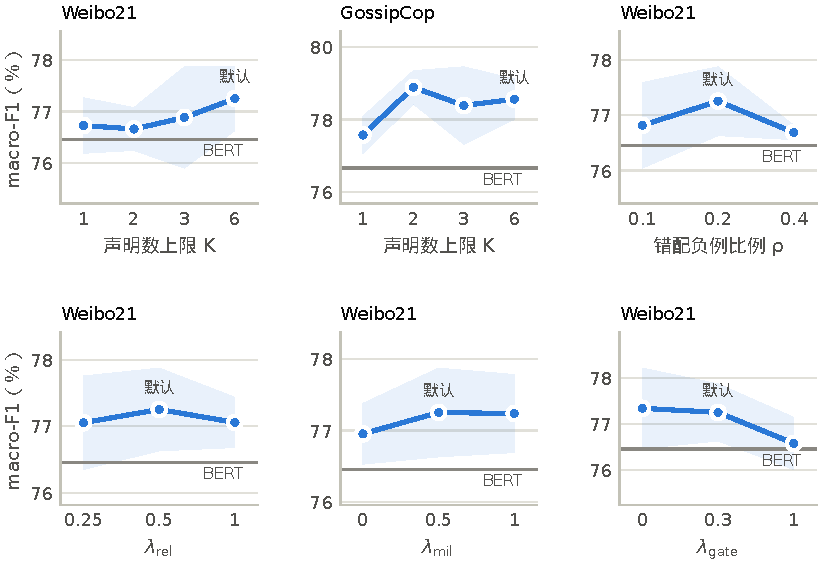
\includegraphics[width=\linewidth]{gen/figures/sensitivity.pdf}
\caption{\method{} 对声明数上限与预设超参数的敏感性}\label{fig:sens}
\note{声明数上限 $K$ 在两个数据集上考察，错配负例比例 $\rho$ 与三个损失权重在 Weibo21 上考察。每个点为 3 个种子的均值，阴影为标准差；标“默认”的点是正文使用的取值在相同 3 个种子上的结果，灰色横线为 BERT。}
\end{figure}

\section{受控测试集的构建细节}\label{app:perturb}

\subsubsection{风格改写}
中文测试集 \cnt{CN/perturb/style_n} 条中有 \cnt{CN/perturb/style_rewritten} 条得到了可用的改写，英文 \cnt{EN/perturb/style_n} 条中为 \cnt{EN/perturb/style_rewritten} 条。被丢弃的主要是改写后长度超过原文 2.5 倍的短消息。作为事实保持程度的粗略代理，我们统计了原文中的数字串在改写后的保留比例：中文为 \pone{CN/fact_preservation/kept_rate}\%，英文为 \pone{EN/fact_preservation/kept_rate}\%。这只是一个代理指标，改写仍可能增删细节，这是 LLM 风格攻击的共同局限\citep{wu2024sheepdog}。

\subsubsection{单句事实篡改}
候选为测试集中至少含两句、且存在长度足够的句子的真新闻（中文 \cnt{CN/perturb/tamper_candidates} 条，英文 \cnt{EN/perturb/tamper_candidates} 条）。篡改模型给出的片段必须在句中恰好出现一次，替换后字母与数字内容必须发生变化，且替换不得改变分句结果。最终得到中文 \cnt{CN/perturb/tamper_n} 条、英文 \cnt{EN/perturb/tamper_n} 条，平均每条分别含 \fone{CN/perturb/tamper_mean_sents} 与 \fone{EN/perturb/tamper_mean_sents} 句。按篡改类型的定位结果见表~\ref{tab:loc-type}。

\begin{table}[htbp]
\centering\small
\caption{按篡改类型划分的定位 Hit@1（\%）}\label{tab:loc-type}
\fittable{gen/tables/loc_type.tex}
\end{table}

\section{样例}\label{app:cases}

下面两条样例按预先固定的规则选出：篡改测试集中按编号排序、含 3--4 句且不超过 170 个字符的前两条，取随机种子 1 的模型输出，未做任何人工挑选。被篡改的句子与其原句用〔〕标出；表中 $+$ 与 $-$ 分别为 LLM 写出的支持论证与质疑论证，$v_k$、$r_k$、$g_k$、$p_k$ 依次为 LLM 的怀疑度、相关性门控、判定门控与实例概率。

两条样例反映了正文中的几点观察。其一，两条篡改后的新闻都没有被判为假（$\hat y$ 接近 0），与表~\ref{tab:tamper} 一致。其二，对应被改句子的声明在各条声明中 $p_k$ 最高，定位是对的，但数值本身远低于 0.5。其三，7B 模型写出的论证质量不稳定：样例 1 中“支持”一栏写的其实是质疑；样例 2 中对应第 3 句的声明，其质疑论证称“具体日期和发言人姓名未明确提及”，而原文两者都有。这条与文本不符的论证并没有被相关性门控关闭：两条样例中所有声明的 $r_k$ 都接近 1。样例 2 的整体实例 $r_0$ 较低（0.40），从单个样例无法判断其原因。

\noindent\textbf{样例 1}（篡改类型：实体；\method{} 预测 $\hat y=0.000$）\par
{\small\begin{quote}
[1] \textbf{〔被篡改〕}【华为隐形指纹技术正式亮相】\quad\textbf{〔原句〕}【vivo隐形指纹技术正式亮相】\par
[2] 全面屏手机时代即将到来。\par
[3] 如此一来前后指纹已成为过去式，所有手机设计上又将站在同一起跑线了，大家觉得屏幕内指纹解锁帅不帅？秒拍视频\par
\end{quote}}
{\small\begin{tabularx}{\linewidth}{@{}clXcccc@{}}
\toprule
句 & 类型 & 声明与两方论证 & $v_k$ & $r_k$ & $g_k$ & $p_k$ \\
\midrule
-- & 整体 & \textbf{这条消息整体的可信度}\newline $+$ 全面屏手机的发展趋势确实存在。\newline $-$ 消息中提到的华为隐形指纹技术未得到官方证实。 & 0.74 & 0.98 & 0.23 & 0.001 \\
1 & 事实 & \textbf{华为隐形指纹技术正式亮相}\newline $+$ 华为经常发布新技术，此消息可能为谣言。\newline $-$ 华为官方未发布过此消息。 & 0.59 & 1.00 & 0.62 & 0.011 \\
2 & 观点 & \textbf{全面屏手机时代即将到来}\newline $+$ 手机厂商都在研发全面屏，此说法有一定合理性。\newline $-$ 全面屏技术仍在发展，尚未普及。 & 0.45 & 1.00 & 0.54 & 0.003 \\
\bottomrule
\end{tabularx}}
\par\medskip
\noindent\textbf{样例 2}（篡改类型：实体；\method{} 预测 $\hat y=0.001$）\par
{\small\begin{quote}
[1] 【天津健康码亮码超2100万次集成新功能后将沿用】\par
[2] 很多人关心疫情过后，天津健康码是否还会沿用？\par
[3] 在3月19日召开的新闻发布会上，天津市大数据管理中心主任边柯柯就此回应称，天津健康码将联合津心办一网通办平台，集成更多便民服务应用，继续沿用下去。\par
[4] \textbf{〔被篡改〕}边柯柯介绍说，天津将积极推动电子通行证在互联网+医疗健康相关场景的应用，实现签约预约\quad\textbf{〔原句〕}边柯柯介绍说，天津将积极推动健康码在互联网+医疗健康相关场景的应用，实现签约预约\par
\end{quote}}
{\small\begin{tabularx}{\linewidth}{@{}clXcccc@{}}
\toprule
句 & 类型 & 声明与两方论证 & $v_k$ & $r_k$ & $g_k$ & $p_k$ \\
\midrule
-- & 整体 & \textbf{这条消息整体的可信度}\newline $+$ 声明直接引用了官方发言，具有较高的可信度。\newline $-$ 消息中提及的具体日期和发言人姓名不明确，且部分内容为预测性意见，缺乏具体细节。 & 0.52 & 0.40 & 0.50 & 0.006 \\
3 & 引述 & \textbf{天津市大数据管理中心主任边柯柯在3月19日的新闻发布会上表示，天津健康码将集成更多便民服务应用，继续沿用下去。}\newline $+$ 该声明直接引用了官方发言，具有较高的可信度。\newline $-$ 新闻发布会的具体日期和发言人姓名未明确提及，可能存在信息不准确的风险。 & 0.23 & 1.00 & 0.82 & 0.007 \\
4 & 观点 & \textbf{天津将积极推动电子通行证在互联网+医疗健康相关场景的应用。}\newline $+$ 这是官方对未来发展的积极展望，符合政策导向。\newline $-$ 该说法是预测性意见，缺乏具体实施细节和时间表，可信度较低。 & 0.64 & 1.00 & 0.89 & 0.034 \\
\bottomrule
\end{tabularx}}
\par\medskip


\chapter{第~\ref{ch:openbook}~章的实现细节}\label{app:ob}

\section{验证器的提示词}\label{app:ob-prompt}

下面是验证器的系统提示与用户提示，以 RAWFC 的三个等级为例；LIAR-RAW 的选项为六个等级（A 至 F）。闭卷的 LoRA-LLM 与零样本基线使用同样的选择题，但没有证据部分，系统提示相应地改为“只给出声明、没有证据”。

{\small\setlength{\parindent}{0pt}\begin{quote}
You are an experienced fact-checker. You are given a claim and sentences retrieved from news reports. Judge how truthful the claim is. Rely on the evidence where it addresses the claim; the evidence may be incomplete, noisy or irrelevant.\par
\vspace{3pt}
Claim: 〈待核查的声明〉\par
\vspace{3pt}
Evidence:\par
[1] (来源域名 1) 〈证据句 1〉\par
[2] (来源域名 2) 〈证据句 2〉\par
……\par
\vspace{3pt}
How truthful is the claim?\par
A. false\par
B. half true\par
C. true\par
Answer with a single letter.\par
\end{quote}}


\section{实现细节}\label{app:ob-impl}

\subsubsection{报道的标记规则}
\ref{sec:ob-audit}~节的五种标记原因按下列规则判断，前四种只看网址。（1）标签来源的核查机构：域名为 snopes.com 或 politifact.com（含子域名）。（2）其他事实核查网站与聚合页：factcheck.org、truthorfiction.com、leadstories.com、checkyourfact.com、fullfact.org、factcheck.afp.com、hoax-slayer.com/net、mediabiasfactcheck.com、rssing.com 等。（3）代码与数据托管站点：github.com、githubusercontent.com、kaggle.com、huggingface.co、paperswithcode.com、gitlab.com、rpubs.com、data.world 等。（4）事实核查栏目：不属于前三类，且网址中含有 fact-check、factcheck、debunk、hoax、pinocchio、truth-o-meter 等字样。（5）正文提及事实核查：报道的任一句子匹配 fact check、fact-checking、Snopes、PolitiFact、pants on fire、truth-o-meter、debunk、Pinocchio 等词。完整的正则表达式见代码仓库中的 \texttt{openbook/data.py}。

\subsubsection{文本预处理与检索}
数据集发布的报道是分词并做过词形还原的文本，我们只还原了标点前后的空格与引号，没有改动词形。BM25 的参数取 $k_1=1.2$、$b=0.75$；检索用的词项为小写化、去停用词并经 Porter 词干提取后的词。证据句超过 60 个词的部分在提示中被截断。

\subsubsection{训练}
优化器为 AdamW，权重衰减为 0，梯度裁剪阈值 1.0，预热步数占总步数的 6\%。带证据的输入约含 840 个词元，每步的微批大小为 2，累积 8 步更新一次；闭卷输入的微批大小为 4，累积 4 步。打分头的偏置初始化为 $-1$，权重初始化为 0。RoBERTa-large 使用 AdamW（权重衰减 0.01）、批大小 16 与混合精度。训练环境与第~\ref{ch:clara}~章相同。

\section{RoBERTa-large 的学习率选择}

\begin{table}[htbp]
\centering\small
\caption{RoBERTa-large 在两个学习率下的验证集与测试集 macro-F1（\%）}\label{tab:ob-slm-grid}
\fittable{gen/ob_tables/slm_grid.tex}
\note{多个随机种子的均值与标准差；加粗的验证集数值对应被选中的配置。}
\end{table}

\section{使用其他证据来源的已发表结果}

表~\ref{tab:ob-other} 列出在同样的声明上、但使用其他证据来源的工作所报告的数值。它们的证据或来自在线搜索引擎，或来自维基百科，或在训练中使用了核查结论文本，与正文表~\ref{tab:ob-main} 中使用数据集原始报道的方法不可直接比较，仅供参考。

\begin{table}[htbp]
\centering\small
\caption{使用其他证据来源的工作在两个数据集的声明上报告的 F1（\%）}\label{tab:ob-other}
\fittable{gen/ob_tables/other.tex}
\note{数值取自各论文；“口径”一列说明其 F1 是各类别 F1 的平均（宏平均），还是宏平均精确率与召回率的调和平均。“LIAR / LIAR-RAW”一列中，使用在线搜索或维基百科的工作评测的是 LIAR 的声明（与 LIAR-RAW 的声明相同）。}
\end{table}


\backmatter
\begin{acknowledgements}

（致谢内容请作者本人撰写。）

\end{acknowledgements}

\chapter{在读期间公开发表论文（著）及科研情况}

（请作者本人按实际情况填写。）


\end{document}
